%!TEX program = lualatex
%!TEX encoding = UTF-8 Unicode  
%!TEX root = chapter05.tex  
\documentclass[main.tex]{subfiles}
\begin{document} 
%----------------------------------------------------------------------------------------
%	CHAPTER 5
%----------------------------------------------------------------------------------------
\cleardoublepage 
\loadgeometry{marginlayout}  
\pagestyle{scrheadings} % Print headers again  
\KOMAoptions{
	headwidth=textwithmarginpar,
	headsepline=true,
	headsepline= 0.5pt,
	footwidth=textwithmarginpar,
}   
\onehalfspacing 
\setcounter{chapter}{4}
%----------------------------------------------------------------------------------------
%	
%----------------------------------------------------------------------------------------

\chapter{Notions de fonctions et résolutions graphiques d'(in)équations}
Les fonctions modélisent le monde.
\section{Définitions}

\begin{example}[le domaine de définition d'une fonction]\hfill 
	\begin{enumerate}[label=\alph*)]
		\item \marginnote{
			\begin{tBox}[leftline=false]
				à lire \og $f$ de $\mathbb{R}$ dans $\mathbb{R}$ qui à $x$ associe $x^3-3x+1$\fg.
			\end{tBox}
		} 
	$f$ est la fonction définie pour tout  $x\in\mathbb{R}$ par $f(x)=x^3-3x+1$. 
		
		On écrit : $f\colon \begin{aligned}[t] \mathbb{R} &\to \mathbb{R}\\
			x&\mapsto x^3-3x+1
		\end{aligned}$.
	
	L'image de $x$ par $f$ est $f(x)=x^3-3x+1$.
	
	L'image de $0$ par $f$ est $f(0)=0^3-3\times 0 + 1=1$
	
	L'image de $-5$ par $f$ est $f(-5)= (-5)^3-3(-5)+1=-109$.
		\item Soit $g\colon t\mapsto\frac{1}{2t-1}$. L'expression $g(t)$ admet des valeurs interdites, on peut choisir  $\mathbb{R}\setminus \{\tfrac{1}{2}\}$ comme domaine de définition de $g$. On écrit $g\colon   \begin{aligned}[t]\mathbb{R}\setminus \{\tfrac{1}{2}\} &\to \mathbb{R}\\
			x&\mapsto x^3-3x+1
		\end{aligned}$.
		\item  \marginnote{
			\begin{tBox}[leftline=false]
				Le domaine de définition peut exclure des nombres qui ne sont pas des valeurs interdites.
			\end{tBox}
		}  Soit fonction $h\colon \begin{aligned}[t] \interval{0}{4} &\to \mathbb{R}\\
			x&\mapsto 2x+3
		\end{aligned}$.  
	
		L'image de $0$ par $h$ est $3$. 
		
		Le nombre $-1$ n'admet pas d'image par $h$. Il n'est pas dans le domaine. 
		\item  \marginnote{
			\begin{tBox}[leftline=false]
				Deux fonctions peuvent avoir la même expression mais pas le même domaine de définition.
			\end{tBox}
		} 
	La fonction $i\colon \begin{aligned}[t] \mathbb{N} &\to \mathbb{R}\\
			x&\mapsto 2x+3
		\end{aligned}$ est définie uniquement sur des valeurs entières.
	\end{enumerate}
\end{example}


\newpage
\begin{definition}[vieillotte]
	Soit un ensemble $D\subset \mathbb{R}$ \sidenote{(généralement un intervalle ou une réunion d'intervalles)}.
	
	Une fonction $f$ définie sur $D$ est une \textbf{relation} qui à tout nombre $x\in D$ \textbf{associe un unique} $y\in \mathbb{R}$. On écrit : 
	\marginnote{
		\begin{tBox}[leftline=false]
		lire \og fonction $f$ de $D$ dans $\mathbb{R}$ qui à $x\in D$ associe $f$ de $x$\fg{}
		\end{tBox}
	} 
\setlength{\abovedisplayskip}{3pt} 
\setlength{\belowdisplayskip}{3pt} 
$$
	f :   \begin{aligned}[t]  D &\to \mathbb{R}\\
		x&\mapsto f(x)
	\end{aligned} 
$$ 
\end{definition}

Dans les cas courants au lycée la relation est décrite par une \textbf{expression} (une règle de calcul) pour calculer l'image $f(x)$ connaissant la valeur de  $x$. Mais beaucoup de fonction n'ont pas d'expression algébrique\sidenote{$d\colon \begin{aligned}[t] \mathbb{N} &\to \mathbb{R}\\
		x&\mapsto \textbf{nbr de diviseurs de $x$}
	\end{aligned}$}. 
\begin{definition} 
	Une fonction $f$ est un \textbf{ensemble de couples} $(x,y)$ ($x$ est l'abscisse, $y$ est l'ordonnée), tel qu'il n'y ait pas 2 couples  ayant la même abscisse mais des ordonnées différentes.
	\setlength{\abovedisplayskip}{3pt}
	\setlength{\belowdisplayskip}{3pt}  
	$$\text{si }   (x,y)\in f\quad \text{ et } (x;y')\in f\quad \text{alors} \quad y=y'$$ 
	Le domaine de $f$ est l'ensemble noté $D_f$ des abscisses de la fonction.  
\end{definition}
Pour tout $x\in\mathbb{R}$, on a 2 possibilités :
\begin{enumerate}[label=\textbullet, leftmargin=*]
	\item L'abscisse $x\notin D_f$ : Il n'existe pas de $y$ tel que $(x,y)\in f$. $x$ n'a pas d'image. 
	\item l'abscisse $x\in D_f$ :  Il existe \textbf{exactement} une  ordonnée $y$  tel que le couple $(x,y)\in f$. On écrit $y=f(x)$ et on dira que \og $y$ est \textbf{l'image} de $x$ \fg{} ou encore \og $x$ est \textbf{un} antécédent de $y$  \fg{}. Noter cette asymétrie.
	
\end{enumerate} 
\begin{figure}[h]\centering
	\begin{tikzpicture}[xscale=0.8, yscale=0.8]
		\tkzSetUpPoint[size=3, fill=black]
		\tkzfctset{tan style/.style={->,>=latex, color=red, line width=1.2pt}}  
		\tkzInit[xmin=-6.0,xmax=6.0,ymin=-3.0,ymax=6.5,xstep=1.0, ystep=1.0];  
		\tkzDrawX[  noticks,label={$x$}, font=\scriptsize, line width=1.2pt , color=blue ]  
		\tkzDrawY[ noticks, label={$y$}, font=\scriptsize, line width=1.2pt , color=red ] 
		\tkzRep[color  = Maroon,xlabel=,ylabel=, font=\scriptsize, line width = 2pt,xnorm=1, ynorm=1]   
		\tkzLabelXY[  font=\scriptsize  ] 
		%		\begin{scope}[dashed] 
			%			\tkzGrid[ xstep=1, ystep=1](-6,-4)(6,7)
			%		\end{scope}
		\begin{scope} 
			\tkzFct[domain = -5.05:0,  line width=1.0pt,*-]{ 
				%			.1*(\x+5)*(\x+2)*(3.25-\x)*exp(\x/6)-1	+ (\x+5)*(\x+2)/(4.2*1.2)*0.214 
				(0.0333*(\x**4)+0.3166*(\x**3)+1.2166*(\x**2)+2.9333*\x+2.0)
			};  
		\end{scope}
		
		%		\tkzText[below right](0,0){O}; 
		%		\tkzText[below ](1,0){1}; 
		%		\tkzText[right](0,1){1};
		\begin{scope} 
			\tkzSetUpPoint[size=3, fill=white]
			\tkzFct[domain = 0.0:5.0,  line width=1.0pt, -]{  
				(-0.0084467165*(\x**6)+0.1395408967*(\x**5)-0.7887193614*(\x**4)+1.863011866*(\x**3)-2.8992653081*(\x**2)+4.6938786232*\x+2.0)
			};  
		\end{scope}
		\tkzDefPoint(-5,-1){P1}
		\tkzDefPoint(-4,-2){P2}
		\tkzDefPoint(-2,-1){P3}
		\tkzDefPoint(-1,-0){P4}
		\tkzDefPoint(0,2){P5}
		\tkzDefPoint(1,5){P6}
		\tkzDefPoint(2,6){P7}
		\tkzDefPoint(4,0){P8}
		\tkzDefPoint(5,-3){P9} 
		
		\tkzPointShowCoord[ xlabel={}, xstyle={} ](P1)
		\tkzPointShowCoord[ xlabel={}, xstyle={} ](P9)
		\tkzPointShowCoord[ xlabel={}, xstyle={} ](P2)
		\tkzPointShowCoord[noydraw](P3)
		\tkzPointShowCoord[ xlabel={}, xstyle={} ](P6)
		\tkzPointShowCoord[ xlabel={}, xstyle={} ](P7)
		\tkzDrawPoints[ color=black, size=5, fill=black, shape=cross ](P1,P2,P3,P4,P5,P6,P7,P8) 
		\tkzDrawPoints[ color=black, size=7, fill=white,  ](P9)
		%		\tkzDrawPoint[ color=black, size=5, fill=black, shape=cross ](P) 
		%		\tkzPointShowCoord(P4)  
		\tkzDefPoint(3,4.15408){P10}  
		\tkzPointShowCoord[   xlabel={\color{blue}$x$}, xstyle={below=6pt} , ylabel={\color{red}$y=f(x)$}, ystyle={left} ](P10)
		\tkzLabelPoint[right](P10){\small$M(x;y)$}	
		\tkzDefPoint(-4.8,-2.5){T1} 
		\tkzText[color = black, above, fill=white](T1){$\mathscr{C}_f$}
		\tkzDefPoint(4.0,-1.5){A1}
		\tkzDefPoint(4.5,0){A2}	
		\tkzLabelPoint[below right](P2){\small$A($}	
		\tkzLabelPoint[below right](P3){\small$B($}
		\tkzDefPoint(3,3.4){Q1}
		\tkzDefPoint(3,5.4){Q2}  
		\tkzPointShowCoord[  ylabel={\color{red}$y'\neq f(x)$}, xstyle={below=6pt}](Q2)
		% 		 		\tkzPointShowCoord[noxdraw, ylabel={\color{red}$y"$},xstyle={below=6pt}](Q1)
		\tkzLabelPoint[right](Q2){\small$N(x;y')\notin  \mathscr{C}_f$} 
		\draw[->,>=latex] (A1) to[bend right=15] (A2);
		\tkzText[color = black, below,  text width=3.8cm](A1){Axe des abscisses, où lire les antécédents}
		\tkzDefPoint(-2.1,6.3){A3}
		\tkzDefPoint(0,6.4){A4}
		\draw[->,>=latex] (A3) to[bend left=15] (A4);
		\tkzText[color = black, left,  text width=3.5cm](A3){Axe des ordonnées où lire l'image}	
	\end{tikzpicture}
	\caption{\label{chap06.fig.fonction}La représentation graphique d'une fonction $f$ dans un repère $(O;I,j)$ est l'ensemble de points notés $\mathscr{C}_f$ :
		$$
		M(u;v)\in\mathscr{C}_f \quad \iff \quad v=f(u)
		$$
		On écrit $
		\mathscr{C}_f\colon y= f(x)
		$. \newline
	La représentation graphique d'une fonction	ne peut pas avoir deux points ayant même abscisse et des ordonnées différentes.}
\end{figure}
%\newpage 
%\begin{definition}
%	La représentation graphique d'une fonction est $f$ dans le plan muni d'un repère, est l'ensemble de points notés $\mathscr{C}_f$ :
%	$$
%	M(u;v)\in\mathscr{C}_f \quad \iff \quad v=f(u)
%	$$
%	On dira que $\mathscr{C}_f$ a pour équation $y=f(x)$, et on écrit :
%	$$
%	\mathscr{C}_f\colon y= f(x)
%	$$
%\end{definition}
%----------------------------------------------------------------------------------------
%	EXERCICES
%----------------------------------------------------------------------------------------

\newpage 
\subsection{TD sudomaths vocabulaire des fonctions}
\paragraph{Objectif} comprendre l'utilisation de $f(x)=y$ dans des formulations diverses.

On se donne une fonction $f$, représentée par la courbe $\mathscr{C}_f$, et définie par une expression $f(x)=2x^2+x+5$.
\begin{enumerate}[leftmargin=*,label=\arabic*)]
\item {questions se ramenant à une recherche d'image $f(x)=?$}
\begin{enumerate}[leftmargin=*,label=\alph*)]
	\item déterminer l'image de $4$ par la fonction $f$
	\item calculer $f(4)$
	\item déterminer l'ordonnée du point de la courbe $\mathscr{C}_f$ d'abscisse $4$ 
	\item Si $x=4$, déterminer la valeur de l'expression  $2x^2+x+5$ 
\end{enumerate}
\item {questions se ramenant à une recherche d'antécédents $f(?)=y$ }
	\begin{enumerate}[leftmargin=*,label=\alph*)]
		\item déterminer les antécédents de $4$ par la fonction $f$
		\item résoudre l'équation $f(x)=4$, inconnue $x$.
		\item résoudre l'équation  $2x^2+x+5=4$, inconnue $x$. 
		\item déterminer les abscisses des points de la courbe $\mathscr{C}_f$ dont l'ordonnée est $4$ 
	\end{enumerate} 
\end{enumerate}
%----------------------------------------------------------------------------------------
%	EXERCICES
%----------------------------------------------------------------------------------------

\newpage 
\paragraph{Histoire des maths}
Le britannique \textbf{William Playfair} fut parmi les premiers à avoir recourt aux représentations graphiques de fonctions. Il est l'inventeur aussi de l'histogramme et du diagramme circulaire (camembert).

\begin{figure*}[!hb]
	\includegraphics[width=0.75\columnwidth]{2ndChap0401.png}
	\includegraphics[width=0.75\columnwidth]{2ndChap0402.png} 
\caption{Playfair dans \og Commercial and Political Atlas \fg de 1786 : Série chronologique du déficit du commerce extérieur (haut) et représentation graphique de l'évolution des intérêts de la dette publique britannique au cours du 18\ieme siècle (bas).}
\end{figure*}
 

%----------------------------------------------------------------------------------------
%	EXERCICES
%----------------------------------------------------------------------------------------

\newpage 
\loadgeometry{widelayout}  
\pagestyle{scrheadings} % Print headers again  
\KOMAoptions{
	headwidth=textwithmarginpar,
	headsepline=true,
	headsepline= 0.5pt,
	footwidth=textwithmarginpar,
} 
\onehalfspacing
\subsection{Exercices : Représentations graphiques, expressions et domaine} 
\begin{example}Complétez les pointillés\hfill
	
\noindent
\parbox{0.48\linewidth}{
\begin{tikzpicture}[xscale=1.0, yscale=1]
	\tkzInit[xmin=-4.0,xmax=4.0,ymin=-3.0,ymax=4.0,xstep=1.0, ystep=1.0];
	\tkzSetUpPoint[size=4, fill=black]
	\tkzfctset{tan style/.style={->,>=latex, color=red, line width=1.2pt}}  
	\begin{scope}[dashed]  
		\tkzGrid[ sub,color=gray,subxstep=1.0,subystep=1.0](-4.0,-3.0)(4.0,4.0);  
	\end{scope}
	\tkzDrawX[above=5pt, label=$x$, font=\scriptsize, line width=1.2pt] 
	\tkzDrawY[right=5pt, label=$y$, font=\scriptsize, line width=1.2pt]
	
	\tkzLabelX[orig=false, font=\scriptsize ]  
	\tkzLabelY[orig=false,  font=\scriptsize] 
	\tkzRep[color  = Maroon,xlabel=,ylabel=, font=\scriptsize, line width = 2pt,xnorm=1, ynorm=1]   
	
	
	
	%	\tkzFct[domain = -7.0:-6.0,  line width=1.0pt]{ 
		%		(-3.6319*(exp(-0.8*(\x+7.0)**6)-0.449328) )
		%	};
	%	\tkzDefPointByFct[ref=P0]({-7.0})		
	%	\tkzFct[domain = -6.0:-1,  line width=1.0pt]{ 
		%		0.01*(\x+6)*(\x+1)**3*(\x-3)*exp(-\x*0.125-0.5)*0.86182 
		%	}; 
	%	\tkzDefPointByFct[ref=P1]({-6})
	%	\tkzDefPointByFct[ref=P2]({-5})
	%	\tkzDefPointByFct[ref=P3]({-1})
	%	\tkzFct[domain = -1:3,  line width=1.0pt]{ 
		%		0.01*(\x+6)*(\x+1)**3*(\x-3)*exp(-\x*0.125-0.5)*0.9801 
		%	};
	%	\tkzDefPointByFct[ref=P4]({2})
	%	\tkzFct[domain = 3:4,  line width=1.0pt]{ 
		%		0.01*(\x+6)*(\x+1)**3*(\x-3)*exp(-\x*0.125-0.5)*0.8698501851 *0.75
		%	};	
	%	\tkzDefPointByFct[ref=P5]({3})
	%	\tkzDefPointByFct[ref=P6]({4})
	%	\tkzDrawPoints(P0, P1, P2, P3, P4, P5, P6);
	%	\tkzPointShowCoord[ xlabel={\color{blue}$-5$}, xstyle={below=8pt} , ylabel={\color{red}$M=f(-5)$}, ystyle={right=8pt} ](P1) 
	%	\tkzPointShowCoord[ xlabel={\color{blue}$2$}, xstyle={above=6pt} , ylabel={\color{red}$m=f(2)$}, ystyle={left} ](P2) 
	
	
%	%	\tkzText[below left](0,0){O};  
%	\tkzDefPoint(4.5,1.5){T1}
%	\tkzText[color = black, above, fill=white](T1){$\mathcal{C}_f$}
%	\tkzText[above right](1,0){\scriptsize $I$}; 
%	\tkzText[above right](0,1){\scriptsize $J$};
	
	% show curve controls, 
	\draw [ line width=2pt]   (-3,1)    
	.. controls ++(-50:1) and ++(-45:-1) ..   (-2,-1) 
	.. controls ++(-45:1) and ++(-35:-1) ..   (-1,-2) 
	.. controls ++(-35:0.5) and ++(-15:-0.5) .. ( 0, -2.5)  
	.. controls ++(0:1) and ++(70:-1) .. ( 2, -1)  
	.. controls ++(70:1) and ++(80:-1) .. ( 3, 2)  ;  
	
	
	\filldraw [draw=black, fill=white, ultra thick] (-3,1)    circle (4pt) ;
	\filldraw [black]  (3,2)     circle (4pt) ; 
\end{tikzpicture}

Domaine : $D=\ldots$


Image de $-1$ : \hfill $f(\ldots)=\ldots$

Image de $3$: \hfill $f(\ldots)=\ldots$


Antécédent(s) de $3$: \hfill $f(\ldots)=\ldots$;  $f(\ldots)=\ldots$

Antécédent(s) de $2$: \hfill $f(\ldots)=\ldots$;  $f(\ldots)=\ldots$

Antécédent(s) de $-1$: \hfill $f(\ldots)=\ldots$;  $f(\ldots)=\ldots$


Image de $0$ : : \hfill $f(\ldots)=\ldots$  

Antécédent(s) de $0$ : \hfill $f(\ldots)=\ldots$ ;  $f(\ldots)=\ldots$
}\hfill 
\parbox{0.48\linewidth}{
\begin{tikzpicture}[ scale=1]
	\tkzInit[xmin=-4.0,xmax=4.0,ymin=-3.0,ymax=4.0,xstep=1.0, ystep=1.0];
	\tkzSetUpPoint[size=4, fill=black]
	\tkzfctset{tan style/.style={->,>=latex, color=red, line width=1.2pt}}  
	\begin{scope}[dashed]  
		\tkzGrid[ sub,color=gray,subxstep=1.0,subystep=1.0](-4.0,-3.0)(4.0,4.0);  
	\end{scope}
	\tkzDrawX[above=5pt, label=$x$, font=\scriptsize, line width=1.2pt] 
	\tkzDrawY[right=5pt, label=$y$, font=\scriptsize, line width=1.2pt]
	
	\tkzLabelX[orig=false, font=\scriptsize ]  
	\tkzLabelY[orig=false,  font=\scriptsize] 
	\tkzRep[color  = Maroon,xlabel=,ylabel=, font=\scriptsize, line width = 2pt,xnorm=1, ynorm=1]   
	
	
	
	%	\tkzFct[domain = -7.0:-6.0,  line width=1.0pt]{ 
		%		(-3.6319*(exp(-0.8*(\x+7.0)**6)-0.449328) )
		%	};
	%	\tkzDefPointByFct[ref=P0]({-7.0})		
	%	\tkzFct[domain = -6.0:-1,  line width=1.0pt]{ 
		%		0.01*(\x+6)*(\x+1)**3*(\x-3)*exp(-\x*0.125-0.5)*0.86182 
		%	}; 
	%	\tkzDefPointByFct[ref=P1]({-6})
	%	\tkzDefPointByFct[ref=P2]({-5})
	%	\tkzDefPointByFct[ref=P3]({-1})
	%	\tkzFct[domain = -1:3,  line width=1.0pt]{ 
		%		0.01*(\x+6)*(\x+1)**3*(\x-3)*exp(-\x*0.125-0.5)*0.9801 
		%	};
	%	\tkzDefPointByFct[ref=P4]({2})
	%	\tkzFct[domain = 3:4,  line width=1.0pt]{ 
		%		0.01*(\x+6)*(\x+1)**3*(\x-3)*exp(-\x*0.125-0.5)*0.8698501851 *0.75
		%	};	
	%	\tkzDefPointByFct[ref=P5]({3})
	%	\tkzDefPointByFct[ref=P6]({4})
	%	\tkzDrawPoints(P0, P1, P2, P3, P4, P5, P6);
	%	\tkzPointShowCoord[ xlabel={\color{blue}$-5$}, xstyle={below=8pt} , ylabel={\color{red}$M=f(-5)$}, ystyle={right=8pt} ](P1) 
	%	\tkzPointShowCoord[ xlabel={\color{blue}$2$}, xstyle={above=6pt} , ylabel={\color{red}$m=f(2)$}, ystyle={left} ](P2) 
	
	
	%	%	\tkzText[below left](0,0){O};  
	%	\tkzDefPoint(4.5,1.5){T1}
	%	\tkzText[color = black, above, fill=white](T1){$\mathcal{C}_f$}
	%	\tkzText[above right](1,0){\scriptsize $I$}; 
	%	\tkzText[above right](0,1){\scriptsize $J$};
	
	% show curve controls, 
	\draw [ line width=2pt]   (-4,3)    
	.. controls ++(-50:1) and ++(-0:-1) ..  (-2,1) ;
	\draw [ line width=2pt]  (-2,-1)
	.. controls ++(-45:1) and ++(-30:-0.5) ..   (-1,-2) 
	.. controls ++(0:1) and ++(-35:-1) ..   (1,2) 
	.. controls ++(-35:0.5) and ++(-15:-0.5) .. ( 3, -2)    ;  
	
	
	\filldraw [draw=black, fill=white, ultra thick] (-2,-1)    circle (4pt) ;
	\filldraw [black]  (3,-2)     circle (4pt)
	(-2,1)     circle (4pt) ; 
\end{tikzpicture}

Domaine : $D=\ldots$


Image de $-2$ : \hfill $f(\ldots)=\ldots$

Image de $\numprint{1.5}$: \hfill $f(\ldots)=\ldots$


Antécédent(s) de $3$: \hfill $f(\ldots)=\ldots$;  $f(\ldots)=\ldots$

Antécédent(s) de $1$: \hfill $f(\ldots)=\ldots$;  $f(\ldots)=\ldots$

Antécédent(s) de $-3$: \hfill $f(\ldots)=\ldots$;  $f(\ldots)=\ldots$


Image de $0$ : : \hfill $f(\ldots)=\ldots$  

Antécédent(s) de $0$ : \hfill $f(\ldots)=\ldots$ ;  $f(\ldots)=\ldots$
} 
\end{example}

\begin{exercise}Complétez. $\mathscr{C}_f$ désigne la courbe représentative de la fonction $f$.
	\vspace{-0.5em}
	\begin{spacing}{2} 
		\begin{enumerate}[label=\arabic*),leftmargin =*]  
			\item $f(2)=3$, l'image de $\ldots\ldots$ est $\ldots\ldots$, et le point $A(\ldots\ldots)\in\mathscr{C}_f$.
			\item $f(\ldots\ldots)=\ldots\ldots$, l'image de $3$ est $-4$, et le point $A(\ldots\ldots)\in\mathscr{C}_f$.
			\item $f(\ldots\ldots)=\ldots\ldots$, l'image de $\ldots\ldots$ est $\ldots\ldots$, et le point $A(2;-3)\in\mathscr{C}_f$.
			\item $f(0)=5$, la courbe $\mathscr{C}_f$ coupe l'axe des (abscisses/ordonnées) au point $A(\ldots\ldots;\ldots\ldots)$.
			\item $f(\ldots\ldots)=\ldots\ldots$. La courbe  $\mathscr{C}_f$ coupe l'axe des abscisses au point $A(2;\ldots\ldots)$.
			\item $f(3)=5$ et $f(6)=2$. Le point $A(3;6)$ est (au-dessus/sur/en dessous) de $\mathscr{C}_f$ 
			\item $f(2)=1$ et $f(1)=3$. Le point $A(1;2)$ est (au-dessus/sur/en dessous) de $\mathscr{C}_f$
			\item $f(-2)\ldots 4$, le point $A(-2;4)$ est au dessus de  $\mathscr{C}_f$
			\item $f(\ldots)\ldots\ldots\ldots$, la courbe $\mathscr{C}_f$ passe en desssous du point $A(-2;3)$.
		\end{enumerate} 
	\end{spacing}
\end{exercise}
\vspace{-1em} 
\begin{exercise}	Soit la fonction $f$ représentée ci-dessous\\ 
	\noindent
	\parbox{0.48\linewidth}{
		\begin{tikzpicture}[xscale=1.05, yscale=1.05]
			\tkzInit[xmin=-4.0,xmax=4.0,ymin=-2.0,ymax=4.0,xstep=1.0, ystep=1.0];
			\tkzSetUpPoint[size=4, fill=black]
			\tkzfctset{tan style/.style={->,>=latex, color=red, line width=1.2pt}}  
			\begin{scope}[dashed]  
				\tkzGrid[ sub,color=gray,subxstep=1.0,subystep=1.0](-4.0,-2.0)(4.0,4.0);  
			\end{scope}
			\tkzDrawX[above=5pt, label=$x$, font=\scriptsize, line width=1.2pt] 
			\tkzDrawY[right=5pt, label=$y$, font=\scriptsize, line width=1.2pt]
			
			\tkzLabelX[orig=false, font=\scriptsize ]  
			\tkzLabelY[orig=false,  font=\scriptsize] 
			\tkzRep[color  = Maroon,xlabel=,ylabel=, font=\scriptsize, line width = 2pt,xnorm=1, ynorm=1]   
			
			
			\tkzFct[domain = -3.0:3.0,  line width=2pt]{ 
				(  (9 - \x**2)**0.5 )
			};
			%	\tkzDefPointByFct[ref=P0]({-7.0})		
			%	\tkzFct[domain = -6.0:-1,  line width=1.0pt]{ 
				%		0.01*(\x+6)*(\x+1)**3*(\x-3)*exp(-\x*0.125-0.5)*0.86182 
				%	}; 
			%	\tkzDefPointByFct[ref=P1]({-6})
			%	\tkzDefPointByFct[ref=P2]({-5})
			%	\tkzDefPointByFct[ref=P3]({-1})
			%	\tkzFct[domain = -1:3,  line width=1.0pt]{ 
				%		0.01*(\x+6)*(\x+1)**3*(\x-3)*exp(-\x*0.125-0.5)*0.9801 
				%	};
			%	\tkzDefPointByFct[ref=P4]({2})
			%	\tkzFct[domain = 3:4,  line width=1.0pt]{ 
				%		0.01*(\x+6)*(\x+1)**3*(\x-3)*exp(-\x*0.125-0.5)*0.8698501851 *0.75
				%	};	
			%	\tkzDefPointByFct[ref=P5]({3})
			%	\tkzDefPointByFct[ref=P6]({4})
			%	\tkzDrawPoints(P0, P1, P2, P3, P4, P5, P6);
			%	\tkzPointShowCoord[ xlabel={\color{blue}$-5$}, xstyle={below=8pt} , ylabel={\color{red}$M=f(-5)$}, ystyle={right=8pt} ](P1) 
			%	\tkzPointShowCoord[ xlabel={\color{blue}$2$}, xstyle={above=6pt} , ylabel={\color{red}$m=f(2)$}, ystyle={left} ](P2) 
			
			
			%	%	\tkzText[below left](0,0){O};  
			%	\tkzDefPoint(4.5,1.5){T1}
			%	\tkzText[color = black, above, fill=white](T1){$\mathcal{C}_f$}
			%	\tkzText[above right](1,0){\scriptsize $I$}; 
			%	\tkzText[above right](0,1){\scriptsize $J$};
			
			% show curve controls, 
			%		\draw [ line width=2pt]   (-3,1)    
			%		.. controls ++(-50:1) and ++(-45:-1) ..   (-2,-1) 
			%		.. controls ++(-45:1) and ++(-35:-1) ..   (-1,-2) 
			%		.. controls ++(-35:0.5) and ++(-15:-0.5) .. ( 0, -2.5)  
			%		.. controls ++(0:1) and ++(70:-1) .. ( 2, -1)  
			%		.. controls ++(70:1) and ++(80:-1) .. ( 3, 2)  ;  
			
			
			%		\filldraw [draw=black, fill=white, ultra thick] (-3,1)    circle (4pt) ;
			\filldraw [black]  (-3,0)     circle (4pt)
			(3,0)     circle (4pt); 
		\end{tikzpicture}
	}\hfill 
	\parbox{0.48\linewidth}{
		\noindent\QCM[VF,Alterne,Stretch=1.0, Largeur=0.75cm]{%
			%		{$70$ est solution de l'équation $x^{300}=1$ d'inconnue $x$}&2,%
			{Domaine est $\interval{0}{3}$}&2,%
			{L'image de $0$ est $-3$}&2,%
			{ $f(3)=0$}&1,%
			{ $f(-2)=f(2)$}&1,% 
			{ $f(1+2)=3$}&1,%
			{ $f(1)> \numprint{2}$}&1,%
			{$2$ admet deux antécédents}&1,%
			{$3$  admet deux antécédents}&2,% 
			{$-2$  admet un antécédent}&2,%  
		}  
	} 
\end{exercise}
\medskip
\begin{exercise}	Soit la fonction $f$ représentée ci-dessous\\
	\noindent
	\parbox{0.48\linewidth}{
		\begin{tikzpicture}[xscale=1.05, yscale=1.05]
			\tkzInit[xmin=-4.0,xmax=4.0,ymin=-3.0,ymax=4.0,xstep=1.0, ystep=1.0];
			\tkzSetUpPoint[size=4, fill=black]
			\tkzfctset{tan style/.style={->,>=latex, color=red, line width=1.2pt}}  
			\begin{scope}[dashed]  
				\tkzGrid[ sub,color=gray,subxstep=1.0,subystep=1.0](-4.0,-3.0)(4.0,4.0);  
			\end{scope}
			\tkzDrawX[above=5pt, label=$x$, font=\scriptsize, line width=1.2pt] 
			\tkzDrawY[right=5pt, label=$y$, font=\scriptsize, line width=1.2pt]
			
			\tkzLabelX[orig=false, font=\scriptsize ]  
			\tkzLabelY[orig=false,  font=\scriptsize] 
			\tkzRep[color  = Maroon,xlabel=,ylabel=, font=\scriptsize, line width = 2pt,xnorm=1, ynorm=1]   
			
			
%			\tkzFct[domain = -3.0:3.0,  line width=1.2pt]{ 
%				(  (9 - \x**2)**0.5 )
%			};
			%	\tkzDefPointByFct[ref=P0]({-7.0})		
			%	\tkzFct[domain = -6.0:-1,  line width=1.0pt]{ 
				%		0.01*(\x+6)*(\x+1)**3*(\x-3)*exp(-\x*0.125-0.5)*0.86182 
				%	}; 
			%	\tkzDefPointByFct[ref=P1]({-6})
			%	\tkzDefPointByFct[ref=P2]({-5})
			%	\tkzDefPointByFct[ref=P3]({-1})
			%	\tkzFct[domain = -1:3,  line width=1.0pt]{ 
				%		0.01*(\x+6)*(\x+1)**3*(\x-3)*exp(-\x*0.125-0.5)*0.9801 
				%	};
			%	\tkzDefPointByFct[ref=P4]({2})
			%	\tkzFct[domain = 3:4,  line width=1.0pt]{ 
				%		0.01*(\x+6)*(\x+1)**3*(\x-3)*exp(-\x*0.125-0.5)*0.8698501851 *0.75
				%	};	
			%	\tkzDefPointByFct[ref=P5]({3})
			%	\tkzDefPointByFct[ref=P6]({4})
			%	\tkzDrawPoints(P0, P1, P2, P3, P4, P5, P6);
			%	\tkzPointShowCoord[ xlabel={\color{blue}$-5$}, xstyle={below=8pt} , ylabel={\color{red}$M=f(-5)$}, ystyle={right=8pt} ](P1) 
			%	\tkzPointShowCoord[ xlabel={\color{blue}$2$}, xstyle={above=6pt} , ylabel={\color{red}$m=f(2)$}, ystyle={left} ](P2) 
			
			
			%	%	\tkzText[below left](0,0){O};  
			%	\tkzDefPoint(4.5,1.5){T1}
			%	\tkzText[color = black, above, fill=white](T1){$\mathcal{C}_f$}
			%	\tkzText[above right](1,0){\scriptsize $I$}; 
			%	\tkzText[above right](0,1){\scriptsize $J$};
			
			% show curve controls, 
			\draw [ line width=2pt]   (-4,-2)    
			.. controls ++(40:1) and ++(60:-1) ..   (-3,0) 
			.. controls ++(70:0.5) and ++(0:-0.5) ..   (-2,1.5) 
			.. controls ++(0:1) and ++(0:-1) .. ( 0, -1.0)  
			.. controls ++(0:0.5) and ++(70:-0.5) .. ( 1.5, 0)  
			.. controls ++(70:1) and ++(70:-1) .. ( 2, 1.5)
			.. controls ++(70:1) and ++(0:-0.5) .. ( 3, 2.5)   ;  
			
			
			%		\filldraw [draw=black, fill=white, ultra thick] (-3,1)    circle (4pt) ;
			\filldraw [black]  (-4,-2.0)     circle (4pt)
			(3,2.5)     circle (4pt); 
		\end{tikzpicture}
	}\hfill 
	\parbox{0.48\linewidth}{
		\noindent\QCM[VF,Alterne,Stretch=1.0, Largeur=0.75cm]{%
			%		{$70$ est solution de l'équation $x^{300}=1$ d'inconnue $x$}&2,%
			{Domaine est $\interval{-3}{3}$}&2,%
			{$f(\numprint{1.5})=2$}&2,%
			{$f(0)=0$}&2,%
			{$f(-2)=f(2)$}&1,% 
			{$f(1+2)=\numprint{2.5}$}&1,%
			{$f(1)>0$}&2,%
			{$\numprint{1}$  admet deux antécédents}&2,%  
			{$-1$ admet deux antécédents}&1,%
			{L'image de l'image de $-3$ est $-1$}&1,%
			{$f(f(2))=0$}&1,%
		}  
	} 
\end{exercise}
\medskip
\begin{exercise}	Soit la fonction $f$ représentée ci-dessous.
	
	\noindent
	\parbox{0.48\linewidth}{
		\begin{tikzpicture}[xscale=1.05, yscale=1.05]
			\tkzInit[xmin=-4.0,xmax=4.0,ymin=-3.0,ymax=4.0,xstep=1.0, ystep=1.0];
			\tkzSetUpPoint[size=4, fill=black]
			\tkzfctset{tan style/.style={->,>=latex, color=red, line width=1.2pt}}  
			\begin{scope}[dashed]  
				\tkzGrid[ sub,color=gray,subxstep=1.0,subystep=1.0](-4.0,-3.0)(4.0,4.0);  
			\end{scope}
			\tkzDrawX[above=5pt, label=$x$, font=\scriptsize, line width=1.2pt] 
			\tkzDrawY[right=5pt, label=$y$, font=\scriptsize, line width=1.2pt]
			
			\tkzLabelX[orig=false, font=\scriptsize ]  
			\tkzLabelY[orig=false,  font=\scriptsize] 
			\tkzRep[color  = Maroon,xlabel=,ylabel=, font=\scriptsize, line width = 2pt,xnorm=1, ynorm=1]   
			
			
		\tkzFct[domain = -4.0:3.5,  line width=1.2pt]{ 
			(  0.5*\x**3-1.5*\x )
				};
		\tkzDefPointByFct[ref=P0]({2.5})		
			%	\tkzFct[domain = -6.0:-1,  line width=1.0pt]{ 
				%		0.01*(\x+6)*(\x+1)**3*(\x-3)*exp(-\x*0.125-0.5)*0.86182 
				%	}; 
			%	\tkzDefPointByFct[ref=P1]({-6})
			%	\tkzDefPointByFct[ref=P2]({-5})
			%	\tkzDefPointByFct[ref=P3]({-1})
			%	\tkzFct[domain = -1:3,  line width=1.0pt]{ 
				%		0.01*(\x+6)*(\x+1)**3*(\x-3)*exp(-\x*0.125-0.5)*0.9801 
				%	};
			%	\tkzDefPointByFct[ref=P4]({2})
			%	\tkzFct[domain = 3:4,  line width=1.0pt]{ 
				%		0.01*(\x+6)*(\x+1)**3*(\x-3)*exp(-\x*0.125-0.5)*0.8698501851 *0.75
				%	};	
			%	\tkzDefPointByFct[ref=P5]({3})
			%	\tkzDefPointByFct[ref=P6]({4})
			%	\tkzDrawPoints(P0, P1, P2, P3, P4, P5, P6);
			%	\tkzPointShowCoord[ xlabel={\color{blue}$-5$}, xstyle={below=8pt} , ylabel={\color{red}$M=f(-5)$}, ystyle={right=8pt} ](P1) 
			%	\tkzPointShowCoord[ xlabel={\color{blue}$2$}, xstyle={above=6pt} , ylabel={\color{red}$m=f(2)$}, ystyle={left} ](P2) 
			
			
			%	%	\tkzText[below left](0,0){O};  
			%	\tkzDefPoint(4.5,1.5){T1}
			%	\tkzText[color = black, above, fill=white](T1){$\mathcal{C}_f$}
			%	\tkzText[above right](1,0){\scriptsize $I$}; 
			%	\tkzText[above right](0,1){\scriptsize $J$};
			
			% show curve controls, 
%			\draw [ line width=2pt]   (-4,-2)    
%			.. controls ++(40:1) and ++(60:-1) ..   (-3,0) 
%			.. controls ++(70:0.5) and ++(0:-0.5) ..   (-2,1.5) 
%			.. controls ++(0:1) and ++(0:-1) .. ( 0, -1.0)  
%			.. controls ++(0:0.5) and ++(70:-0.5) .. ( 1.5, 0)  
%			.. controls ++(70:1) and ++(70:-1) .. ( 2, 1.5)
%			.. controls ++(70:1) and ++(0:-0.5) .. ( 3, 2.5)   ;  
			
			
			%		\filldraw [draw=black, fill=white, ultra thick] (-3,1)    circle (4pt) ;
%			\filldraw [black]  (-4,-2.0)     circle (4pt) ; 
		\end{tikzpicture}
	}\hfill 
	\parbox{0.48\linewidth}{
		\begin{enumerate}[label=\arabic*),leftmargin=*]
			\item Donner  le domaine de $f$ : \dotfill
			\item Donner l'image de $2$ :\dotfill $f(\ldots)=\ldots$ .
			\item Donner l'image de $0$ : \dotfill 
			\item Donner les antécédents de $-1$\dotfill
			\item Combien a $0$ d'antécédents ?\dotfill
			\item Quel est le nombre d'antécédents de $-2$ ?\dotfill
		\end{enumerate}
		
		
		
		\noindent\QCM[VF,Alterne,Stretch=1.0, Largeur=0.75cm]{%
			%		{$70$ est solution de l'équation $x^{300}=1$ d'inconnue $x$}&2,% 
			{$f(-2)=-f(2)$}&1,% 
			{$f(-1)= f(1)$}&1,%
			{$f(2)=2f(1)$}&1,%  
			{$f(3)>4$}&1,%
			{$f(-1)>0$}&1,%
		}  
	} 
\end{exercise} 

%\begin{example}\hfill 
%	
%\noindent
%\parbox{0.48\linewidth}{
%	\begin{tikzpicture}[xscale=1.0, yscale=1.0]
%		\tkzInit[xmin=-4.0,xmax=4.0,ymin=-3.0,ymax=4.0,xstep=1.0, ystep=1.0];
%		\tkzSetUpPoint[size=4, fill=black]
%		\tkzfctset{tan style/.style={->,>=latex, color=red, line width=1.2pt}}  
%		\begin{scope}[dashed]  
%			\tkzGrid[ sub,color=gray,subxstep=1.0,subystep=1.0](-4.0,-3.0)(4.0,4.0);  
%		\end{scope}
%		\tkzDrawX[above=5pt, label=$x$, font=\scriptsize, line width=1.2pt] 
%		\tkzDrawY[right=5pt, label=$y$, font=\scriptsize, line width=1.2pt]
%		
%		\tkzLabelX[orig=false, font=\scriptsize ]  
%		\tkzLabelY[orig=false,  font=\scriptsize] 
%		\tkzRep[color  = Maroon,xlabel=,ylabel=, font=\scriptsize, line width = 2pt,xnorm=1, ynorm=1]   
%		
%		 
%	\end{tikzpicture}
%}
%\hfill 
%\parbox{0.48\linewidth}{
%Représente dans le repère ci-contre une fonction $f$  tel que :
%\begin{enumerate}[label=\textbullet, leftmargin=*]
%	\item Domaine de $f$ est $\interval{-2}{3}$
%	\item L'image de $-2$ est $3$
%	\item $A(-1,1)$ est un point de $\mathscr{C}_f$.
%	\item $f(0)<0$.
%	\item Si $x\in\interval{0}{1}$ alors $f(x)>-1$.
%	\item $B(2;1)$ est en dessous de  $\mathscr{C}_f$.
%	\item $f(3)=-2$.
%\end{enumerate}
%} 
%\end{example}

\begin{exercise} \hfill 
	
	
	\noindent
	\parbox{0.24\linewidth}{ 
		\begin{tikzpicture}[xscale=0.5, yscale=0.5]
			\tkzInit[xmin=-4.0,xmax=4.0,ymin=-3.0,ymax=4.0,xstep=1.0, ystep=1.0];
			\tkzSetUpPoint[size=4, fill=black]
			\tkzfctset{tan style/.style={->,>=latex, color=red, line width=1.2pt}}  
			\begin{scope}[dashed]  
				\tkzGrid[ sub,color=gray,subxstep=1.0,subystep=1.0](-4.0,-3.0)(4.0,4.0);  
			\end{scope}
			\tkzDrawX[above=5pt, label=$x$, font=\scriptsize, line width=1.2pt] 
			\tkzDrawY[right=5pt, label=$y$, font=\scriptsize, line width=1.2pt]
			
			\tkzLabelX[orig=false, font=\scriptsize ]  
			\tkzLabelY[orig=false,  font=\scriptsize] 
			\tkzRep[color  = Maroon,xlabel=,ylabel=, font=\scriptsize, line width = 2pt,xnorm=1, ynorm=1]   
			
			
			%	%	\tkzText[below left](0,0){O};  
			%	\tkzDefPoint(4.5,1.5){T1}
			%	\tkzText[color = black, above, fill=white](T1){$\mathcal{C}_f$}
			%	\tkzText[above right](1,0){\scriptsize $I$}; 
			%	\tkzText[above right](0,1){\scriptsize $J$};
			
			% show curve controls,  
			\draw [ line width=2pt]  (-3,1)
			.. controls ++(-45:1) and ++(-0:-1) ..   (-1,-2) 
			.. controls ++(0:1) and ++(-35:-1) ..   (1,2) 
			.. controls ++(-35:0.5) and ++(-15:-0.5) .. ( 3, -2)    ;  
			
			
			\filldraw [draw=black, fill=white, ultra thick] (3,-2)    circle (4pt) ;
			\filldraw [black]  (-3,1)     circle (4pt) ; 
		\end{tikzpicture} 
	} 
	\parbox{0.24\linewidth}{ 
		\begin{tikzpicture}[xscale=0.5, yscale=0.5]
			\tkzInit[xmin=-4.0,xmax=4.0,ymin=-3.0,ymax=4.0,xstep=1.0, ystep=1.0];
			\tkzSetUpPoint[size=4, fill=black]
			\tkzfctset{tan style/.style={->,>=latex, color=red, line width=1.2pt}}  
			\begin{scope}[dashed]  
				\tkzGrid[ sub,color=gray,subxstep=1.0,subystep=1.0](-4.0,-3.0)(4.0,4.0);  
			\end{scope}
			\tkzDrawX[above=5pt, label=$x$, font=\scriptsize, line width=1.2pt] 
			\tkzDrawY[right=5pt, label=$y$, font=\scriptsize, line width=1.2pt]
			
			\tkzLabelX[orig=false, font=\scriptsize ]  
			\tkzLabelY[orig=false,  font=\scriptsize] 
			\tkzRep[color  = Maroon,xlabel=,ylabel=, font=\scriptsize, line width = 2pt,xnorm=1, ynorm=1]   
			
			
			
			\tkzFct[domain = -2.0:4.0,  line width=2.0pt]{ 
				( 6*\x/5-2 )
			}; 
			
			%	%	\tkzText[below left](0,0){O};  
			%	\tkzDefPoint(4.5,1.5){T1}
			%	\tkzText[color = black, above, fill=white](T1){$\mathcal{C}_f$}
			%	\tkzText[above right](1,0){\scriptsize $I$}; 
			%	\tkzText[above right](0,1){\scriptsize $J$};
			
			% show curve controls,  
			%		\draw [ line width=2pt]  (-3,1)
			%		.. controls ++(-45:1) and ++(-0:-1) ..   (-1,-2) 
			%		.. controls ++(0:1) and ++(-35:-1) ..   (1,2) 
			%		.. controls ++(-35:0.5) and ++(-15:-0.5) .. ( 3, -2)    ;  
			%		
			%		
			%		\filldraw [draw=black, fill=white, ultra thick] (3,-2)    circle (4pt) ;
			%		\filldraw [black]  (-3,1)     circle (4pt) ; 
		\end{tikzpicture} 
	} 
	\parbox{0.24\linewidth}{ 
		\begin{tikzpicture}[xscale=0.5, yscale=0.5]
			\tkzInit[xmin=-4.0,xmax=4.0,ymin=-3.0,ymax=4.0,xstep=1.0, ystep=1.0];
			\tkzSetUpPoint[size=4, fill=black]
			\tkzfctset{tan style/.style={->,>=latex, color=red, line width=1.2pt}}  
			\begin{scope}[dashed]  
				\tkzGrid[ sub,color=gray,subxstep=1.0,subystep=1.0](-4.0,-3.0)(4.0,4.0);  
			\end{scope}
			\tkzDrawX[above=5pt, label=$x$, font=\scriptsize, line width=1.2pt] 
			\tkzDrawY[right=5pt, label=$y$, font=\scriptsize, line width=1.2pt]
			
			\tkzLabelX[orig=false, font=\scriptsize ]  
			\tkzLabelY[orig=false,  font=\scriptsize] 
			\tkzRep[color  = Maroon,xlabel=,ylabel=, font=\scriptsize, line width = 2pt,xnorm=1, ynorm=1]   
			
			
			
			%		\tkzFct[domain = -2.0:4.0,  line width=2.0pt]{ 
				%			( 6*\x/5-2 )
				%		}; 
			
			%	%	\tkzText[below left](0,0){O};  
			%	\tkzDefPoint(4.5,1.5){T1}
			%	\tkzText[color = black, above, fill=white](T1){$\mathcal{C}_f$}
			%	\tkzText[above right](1,0){\scriptsize $I$}; 
			%	\tkzText[above right](0,1){\scriptsize $J$};
			
			% show curve controls,  
			\draw [ line width=2pt]  (-4,-2)
			.. controls ++(-45:1) and ++(-0:-1) ..   (0,3) 
			.. controls ++(0:1) and ++(90:1) ..   (2,1) 
			.. controls ++(-90:1) and ++(-35:-1) ..   (1,-1) 
			.. controls ++(-35:0.5) and ++(-15:-0.5) .. ( 3, -2)    ;  
			%		
			%		
			\filldraw [draw=black, fill=white, ultra thick] (-4,-2)    circle (4pt) ;
			\filldraw [black]  (3,-2)     circle (4pt) ; 
		\end{tikzpicture} 
	}  
	\parbox{0.24\linewidth}{ 
		\begin{tikzpicture}[xscale=0.5, yscale=0.5]
			\tkzInit[xmin=-4.0,xmax=4.0,ymin=-3.0,ymax=4.0,xstep=1.0, ystep=1.0];
			\tkzSetUpPoint[size=4, fill=black]
			\tkzfctset{tan style/.style={->,>=latex, color=red, line width=1.2pt}}  
			\begin{scope}[dashed]  
				\tkzGrid[ sub,color=gray,subxstep=1.0,subystep=1.0](-4.0,-3.0)(4.0,4.0);  
			\end{scope}
			\tkzDrawX[above=5pt, label=$x$, font=\scriptsize, line width=1.2pt] 
			\tkzDrawY[right=5pt, label=$y$, font=\scriptsize, line width=1.2pt]
			
			\tkzLabelX[orig=false, font=\scriptsize ]  
			\tkzLabelY[orig=false,  font=\scriptsize] 
			\tkzRep[color  = Maroon,xlabel=,ylabel=, font=\scriptsize, line width = 2pt,xnorm=1, ynorm=1]   
			
			
			
			%		\tkzFct[domain = -2.0:4.0,  line width=2.0pt]{ 
				%			( 6*\x/5-2 )
				%		}; 
			
			%	%	\tkzText[below left](0,0){O};  
			%	\tkzDefPoint(4.5,1.5){T1}
			%	\tkzText[color = black, above, fill=white](T1){$\mathcal{C}_f$}
			%	\tkzText[above right](1,0){\scriptsize $I$}; 
			%	\tkzText[above right](0,1){\scriptsize $J$};
			
			% show curve controls,  
			\draw [ line width=2pt]  (-4,2)
			.. controls ++(0:1) and ++(0:-1) ..   (1,2)     ;  
			\draw [ line width=2pt]  (1,1)
			.. controls ++(0:1) and ++(0:-1) ..   (2,1)     ;  
			\draw [ line width=2pt]  (2,-2)
			.. controls ++(0:1) and ++(0:-1) ..   (3,-2)     ;  
			%		
			%		
			\filldraw [draw=black, fill=white, ultra thick] ( 1,2)    circle (4pt) 
			(2,-2)    circle (4pt) 
			(3,-2)    circle (4pt);
			\filldraw [black]  (1,1)     circle (4pt)
			(2,1)     circle (4pt) ; 
		\end{tikzpicture} 
	} 
	
	\begin{enumerate}[label=\arabic*),leftmargin=*]
		\item 	Parmi ces graphiques, lesquels correspondent à la représentation graphique d’une fonction ?
		\item Pour chaque fonction donnez leur domaine et l'image de $2$.
		\item Pour chaque fonction donnez le nombre d'antécédents de $1$. 
	\end{enumerate}
	
\end{exercise}
\begin{exercise}Complétez. $\mathscr{C}_f$ désigne la courbe représentative de la fonction $f$.
	\vspace{-0.5em}
	\begin{spacing}{2} 
		\begin{enumerate}[label=\arabic*),leftmargin =*]  
			\item $f$ définie sur $\mathbb{R}$ par  $f(x)=-5x+3$. $f(0)=\dotfill $
			\item $f$ définie sur $\mathbb{R}$ par  $f(x)=2x^2-3x+5$. $f(-2)=\dotfill $
			\item $f$ définie sur $\mathbb{R}$ par $f(x)=3x-5$. $f(-1)=$\dotfill et $A(\ldots\ldots;\ldots\ldots)\in\mathscr{C}_f$.
			\item $f$ définie sur $\mathbb{R}$ par  $f(x)=x^3-2x+1$. $f(-2)=\dotfill $et $A(\ldots\ldots;\ldots\ldots)\in\mathscr{C}_f$.
			\item $f$ définie sur $\mathbb{R}$ par  $f(x)=3x+p$. Si $f(0)=4$, alors $p=$\dotfill 
			\item $f$ définie sur $\mathbb{R}$ par  $f(x)=2x+p$. Si $f(-1)=-4$, alors $p=$\dotfill 
			\item $f$ définie sur $\mathbb{R}$ par  $f(x)=mx-1$. Si $f(-2)=3$, alors $m=$\dotfill 
			\item $f$ définie sur $\mathbb{R}$ par  $f(x)=mx-4$. Si $f(2)=8$, alors $m=$\dotfill 
			\item $f$ définie sur $\mathbb{R}$ par  $f(x)=x^3-2x-2$. Le point $A(2;1)$ est (au dessus/sur/en dessous) $\mathscr{C}_f$. 
			\item $f(x)=\frac{1}{x}$ n'est pas définie lorsque le dénominateur est nul. Son domaine est $D=\mathbb{R}\setminus $\dotfill  
			\item $f(x)=\frac{1}{2x-3}$ n'est pas définie lorsque $\ldots\ldots\ldots\ldots=0$. Son domaine est $D=\mathbb{R}\setminus $\dotfill 
			\item $f(x)=\sqrt{2x-3}$ n'est définie que si $\ldots\ldots\ldots\ldots\geqslant 0$. Son domaine est $D= $\dotfill  
			\item $f(x)=\sqrt{-5x+1}$ n'est définie que si $\ldots\ldots\ldots\ldots\geqslant 0$. Son domaine est $D= $\dotfill 
			\item Si $T(x)$ est la température de la classe à l'heure $x$ de la journée, son domaine est $D=\dotfill $. 
		\end{enumerate} 
	\end{spacing}
\end{exercise}
\vspace{-2em}
\begin{exercise}  \hfill \\
	 Soit la famille de fonction $f$ définie pour tout $x\in\mathbb{R}$ par $f_m(x)=mx+3m-2$.
 	\begin{enumerate}[label=\arabic*),leftmargin=*]
 		\item Pour $m=2$. Calculer $f(0)$ et $f(-5)$. 
 		\item Sachant que $f(2)=0$, trouvez $m$.
 	\end{enumerate}
 \end{exercise}
 \begin{exercise} Soit la fonction $f$ d'expression $f(x)=\tfrac{1}{x-1}+\tfrac{1}{x+1}$. 
	\begin{enumerate}[label=\arabic*),leftmargin=*]
	\item Déterminez les valeurs $x$ pour lesquelles l'expression n'est pas définie.
	\item En déduire le domaine de définition le plus large possible pour $f$.
\end{enumerate} 
 \end{exercise}  

\begin{exercise}\label{chapter04:exercice:representationexpression} Représentez les fonctions données par leur expression et leur domaine
\end{exercise}  
\noindent  \hfill
$f(x)=4x+1$ pour $x\in\interval{-3}{2}$
\hfill 
$f(x)=5x-6$  pour $x\in\interval{-1}{3}$
\hfill \null

\noindent 
\parbox{0.15\linewidth}{
	\begin{tabularx}{1\linewidth}{?c?Y?}\hline
		$  x $& $f(x)$ \\ \hline 
		$-3$&  \\ \hline
		$-2$&  \\ \hline
		$-1$&  \\ \hline
		$0$&  \\ \hline
		$1$&  \\ \hline
		$2$&  \\ \hline 
	\end{tabularx}
}
\parbox{0.38\linewidth}{ 
	\begin{tikzpicture}[xscale=0.80, yscale=1.5]
		%----------------------- 
		\tkzSetUpPoint[size=3, fill=black]
		\tkzfctset{tan style/.style={->,>=latex, color=red, line width=1.2pt}}  
		\tkzInit[xmin=-4,xmax=3,ymin=-12,ymax=10,xstep=1.0, ystep=4.0  ];
		\tkzGrid[color=gray, line width=0.5pt,]
		\begin{scope}[dashed] 
			\tkzGrid[sub,subxstep=1, subystep=1,color=gray, line width=0.5pt, ]
		\end{scope}  
		\tkzDrawX[  noticks, font=\scriptsize, line width=2pt, label=$x$, above =5pt  ] 
		\tkzDrawY[  noticks,  font=\scriptsize, line width=2pt , up space=0.2pt, label={$y$}, right=5pt, ]  
		\tkzLabelXY[orig = false,  font=\scriptsize]
		 
%		\tkzFct[domain = -3.0:2.0, line width=2pt,samples=100,color = red]{(4*\x+1)}    
		%-----------------------  
	\end{tikzpicture} 
}
\parbox{0.15\linewidth}{
	\begin{tabularx}{1\linewidth}{?c?Y?}\hline
		$  x $& $f(x)$ \\ \hline
		$-2$&  \\ \hline
		$-1$&  \\ \hline
		$0$&  \\ \hline
		$1$&  \\ \hline
		$2$&  \\ \hline
		$3$&  \\ \hline 
	\end{tabularx}
}
\parbox{0.27\linewidth}{ 
	\begin{tikzpicture}[xscale=0.85, yscale=0.75]
		%----------------------- 
		\tkzSetUpPoint[size=3, fill=black]
		\tkzfctset{tan style/.style={->,>=latex, color=red, line width=1.2pt}}  
		\tkzInit[xmin=-2,xmax=3,ymin=-12,ymax=10,xstep=1.0, ystep=2.0  ];
		\tkzGrid[color=gray, line width=0.5pt,]
		\begin{scope}[dashed] 
			\tkzGrid[sub,subxstep=1, subystep=1,color=gray, line width=0.5pt, ]
		\end{scope}  
		\tkzDrawX[  noticks, font=\scriptsize, line width=2pt, label=$x$, above =5pt  ] 
		\tkzDrawY[  noticks,  font=\scriptsize, line width=2pt , up space=0.15pt, label={$y$}, right=5pt, ]  
		\tkzLabelXY[orig = false,  font=\scriptsize]
  
%		\tkzFct[domain = -1.0:3.0, line width=2pt,samples=100,color = red]{(5*\x-6)}   
		%-----------------------  
	\end{tikzpicture} 
}



\noindent  \hfill
$f(x)=-3x+4$ pour $x\in\interval{-3}{3}$
\hfill 
$f(x)=-2x+5$  pour $x\in\interval{-1}{4}$
\hfill \null

\noindent 
\parbox{0.15\linewidth}{
	\begin{tabularx}{1\linewidth}{?c?Y?}\hline
		$  x $& $f(x)$ \\ \hline  
		$-3$&  \\ \hline
		$-2$&  \\ \hline
		$-1$&  \\ \hline
		$0$&  \\ \hline
		$1$&  \\ \hline
		$2$&  \\ \hline 
		$3$&  \\ \hline
	\end{tabularx}
}
\parbox{0.38\linewidth}{ 
	\begin{tikzpicture}[xscale=0.70, yscale=1.2]
		%----------------------- 
		\tkzSetUpPoint[size=3, fill=black]
		\tkzfctset{tan style/.style={->,>=latex, color=red, line width=1.2pt}}  
		\tkzInit[xmin=-4,xmax=4,ymin=-10,ymax=15,xstep=1.0, ystep=5.0  ];
		\tkzGrid[color=gray, line width=0.5pt,]
		\begin{scope}[dashed] 
			\tkzGrid[sub,subxstep=1, subystep=1,color=gray, line width=0.5pt, ]
		\end{scope}  
		\tkzDrawX[  noticks, font=\scriptsize, line width=2pt, label=$x$, above =5pt  ] 
		\tkzDrawY[  noticks,  font=\scriptsize, line width=2pt , up space=0.2pt, label={$y$}, right=5pt, ]  
		\tkzLabelXY[orig = false,  font=\scriptsize]
	 
%		\tkzFct[domain = -3.0:3.0, line width=2pt,samples=100,color = red]{(-3*\x+4)}    
		%-----------------------  
	\end{tikzpicture} 
}
\parbox{0.15\linewidth}{
	\begin{tabularx}{1\linewidth}{?c?Y?}\hline
		$  x $& $f(x)$ \\ \hline
		$-1$&  \\ \hline 
		$0$&  \\ \hline 
		$1$&  \\ \hline 
		$2$ &  \\ \hline
		$3$ &  \\ \hline
	\end{tabularx}
}
\parbox{0.27\linewidth}{ 
	\begin{tikzpicture}[xscale=0.85, yscale=1]
		%----------------------- 
		\tkzSetUpPoint[size=3, fill=black]
		\tkzfctset{tan style/.style={->,>=latex, color=red, line width=1.2pt}}  
		\tkzInit[xmin=-2,xmax=4,ymin=-4,ymax=8,xstep=1.0, ystep=2.0  ];
		\tkzGrid[color=gray, line width=0.5pt,]
		\begin{scope}[dashed] 
			\tkzGrid[sub,subxstep=1, subystep=1,color=gray, line width=0.5pt, ]
		\end{scope}  
		\tkzDrawX[  noticks, font=\scriptsize, line width=2pt, label=$x$, above =5pt  ] 
		\tkzDrawY[  noticks,  font=\scriptsize, line width=2pt , up space=0.15pt, label={$y$}, right=5pt, ]  
		\tkzLabelXY[orig = false,  font=\scriptsize]
	   
%				\tkzFct[domain = -1.0:4.0, line width=2pt,samples=100,color = red]{(-2*\x+5)}   
		%-----------------------  
	\end{tikzpicture} 
}
 

\noindent  \hfill
$f(x)=-x^2+x+6$ pour $x\in\interval{-2}{3}$
\hfill 
$f(x)=x^2 -4x+4$ pour $x\in\interval{-1}{3}$
\hfill \null

\noindent 
\parbox{0.15\linewidth}{
	\begin{tabularx}{1\linewidth}{?c?Y?}\hline
		$  x $& $f(x)$ \\ \hline
		$-2$&  \\ \hline
		$-1$&  \\ \hline
		$0$&  \\ \hline
		$0.5$&  \\ \hline
		$1$&  \\ \hline
		$1.5$&  \\ \hline
		$2$&  \\ \hline 
		$3$&  \\ \hline 
	\end{tabularx}
}
\parbox{0.38\linewidth}{ 
	\begin{tikzpicture}[xscale=0.9, yscale=1.2]
		%----------------------- 
		\tkzSetUpPoint[size=3, fill=black]
		\tkzfctset{tan style/.style={->,>=latex, color=red, line width=1.2pt}}  
		\tkzInit[xmin=-3,xmax=4,ymin=-2,ymax=8,xstep=1.0, ystep=2.0  ];
		\tkzGrid[color=gray, line width=0.5pt,]
		\begin{scope}[dashed] 
			\tkzGrid[sub,subxstep=1, subystep=1,color=gray, line width=0.5pt, ]
		\end{scope}  
		\tkzDrawX[  noticks, font=\scriptsize, line width=2pt, label=$x$, above =5pt  ] 
		\tkzDrawY[  noticks,  font=\scriptsize, line width=2pt , up space=0.2pt, label={$y$}, right=5pt, ]  
		\tkzLabelXY[orig = false,  font=\scriptsize]
	 
%		\tkzFct[domain = -2.0:3.0, line width=2pt,samples=100,color = blue]{(-1*\x**2+1*\x+6)} 
%		\tkzFct[domain = -5.0:6.0, line width=2pt,samples=100,color = red]{(1*\x+10)}    
		%-----------------------  
	\end{tikzpicture} 
}
\parbox{0.15\linewidth}{
	\begin{tabularx}{1\linewidth}{?c?Y?}\hline
		$  x $& $f(x)$ \\ \hline
		$-1$&  \\ \hline
		$0$&  \\ \hline
		$1$&  \\ \hline
		$1.5$&  \\ \hline
		$2$&  \\ \hline
		$2.5$&  \\ \hline
		$3$ &  \\ \hline
	\end{tabularx}
}
\parbox{0.27\linewidth}{ 
	\begin{tikzpicture}[xscale=0.8, yscale=1.75  ]
		%----------------------- 
		\tkzSetUpPoint[size=3, fill=black]
		\tkzfctset{tan style/.style={->,>=latex, color=red, line width=1.2pt}}  
		\tkzInit[xmin=-2,xmax=4,ymin=-5,ymax=10,xstep=1.0, ystep=5.0  ];
		\tkzGrid[color=gray, line width=0.5pt,]
		\begin{scope}[dashed] 
			\tkzGrid[sub,subxstep=1, subystep=1,color=gray, line width=0.5pt, ]
		\end{scope}  
		\tkzDrawX[  noticks, font=\scriptsize, line width=2pt, label=$x$, above =5pt  ] 
		\tkzDrawY[  noticks,  font=\scriptsize, line width=2pt , up space=0.15pt, label={$y$}, right=5pt, ]  
		\tkzLabelXY[orig = false,  font=\scriptsize]
		%	\tkzRep[color  = Maroon,line width = 2pt, posxlabel=below, posylabel=left, xnorm=1, ynorm=1]
		%----------------------- 
%		\tkzFct[domain = -1.0:3.0, line width=2pt,samples=100,color = blue]{(1*\x**2-4*\x+4)}    
		%-----------------------  
	\end{tikzpicture} 
}  
\begin{eBox} 
	Pour tracer la représentation d'une fonction affine $f(x)=mx+p$ définie sur le domaine $\interval{a}{b}$, on trace le \dotfill reliant les points $A(\ldots\ldots;\ldots\ldots)$ et $B(\ldots\ldots;\ldots\ldots)$.
\end{eBox} 
\noindent  \hfill
$f(x)=2x^2+6x$ pour $x\in\interval{-4}{2}$
\hfill 
$f(x)=-2x^2 +4x$ pour $x\in\interval{-1}{2}$
\hfill \null

\noindent 
\parbox{0.15\linewidth}{
	\begin{tabularx}{1\linewidth}{?c?Y?}\hline
		$  x $& $f(x)$ \\ \hline
		$-4$&  \\ \hline
		$-3$&  \\ \hline
		$-2$&  \\ \hline
		$-1$&  \\ \hline
		$0$&  \\ \hline
		$1$&  \\ \hline
		$2$&  \\ \hline 
	\end{tabularx}
}
\parbox{0.38\linewidth}{ 
	\begin{tikzpicture}[xscale=0.70, yscale=1.2]
		%----------------------- 
		\tkzSetUpPoint[size=3, fill=black]
		\tkzfctset{tan style/.style={->,>=latex, color=red, line width=1.2pt}}  
		\tkzInit[xmin=-5,xmax=3,ymin=-5,ymax=20,xstep=1.0, ystep=5.0  ];
		\tkzGrid[color=gray, line width=0.5pt,]
		\begin{scope}[dashed] 
			\tkzGrid[sub,subxstep=1, subystep=1,color=gray, line width=0.5pt, ]
		\end{scope}  
		\tkzDrawX[  noticks, font=\scriptsize, line width=2pt, label=$x$, above =5pt  ] 
		\tkzDrawY[  noticks,  font=\scriptsize, line width=2pt , up space=0.2pt, label={$y$}, right=5pt, ]  
		\tkzLabelXY[orig = false,  font=\scriptsize]
		%	\tkzRep[color  = Maroon,line width = 2pt, posxlabel=below, posylabel=left, xnorm=1, ynorm=1]
		%----------------------- 
%		\tkzFct[domain = -4.0:2.0, line width=2pt,samples=100,color = blue]{(2*\x**2+6*\x)} 
		%		\tkzFct[domain = -5.0:6.0, line width=2pt,samples=100,color = red]{(5*\x)}    
		%-----------------------  
	\end{tikzpicture} 
}
\parbox{0.15\linewidth}{
	\begin{tabularx}{1\linewidth}{?c?Y?}\hline
		$  x $& $f(x)$ \\ \hline
		$-1$&  \\ \hline
		$-0.5$&  \\ \hline
		$0$&  \\ \hline
		$0.5$&  \\ \hline
		$1$&  \\ \hline
		$1.5$&  \\ \hline
		$2$ &  \\ \hline
	\end{tabularx}
}
\parbox{0.27\linewidth}{ 
	\begin{tikzpicture}[xscale=0.85, yscale=1]
		%----------------------- 
		\tkzSetUpPoint[size=3, fill=black]
		\tkzfctset{tan style/.style={->,>=latex, color=red, line width=1.2pt}}  
		\tkzInit[xmin=-2,xmax=3,ymin=-8,ymax=4,xstep=1.0, ystep=2.0  ];
		\tkzGrid[color=gray, line width=0.5pt,]
		\begin{scope}[dashed] 
			\tkzGrid[sub,subxstep=1, subystep=1,color=gray, line width=0.5pt, ]
		\end{scope}  
		\tkzDrawX[  noticks, font=\scriptsize, line width=2pt, label=$x$, above =5pt  ] 
		\tkzDrawY[  noticks,  font=\scriptsize, line width=2pt , up space=0.15pt, label={$y$}, right=5pt, ]  
		\tkzLabelXY[orig = false,  font=\scriptsize]
		%	\tkzRep[color  = Maroon,line width = 2pt, posxlabel=below, posylabel=left, xnorm=1, ynorm=1]
		%----------------------- 
%		\tkzFct[domain = -1.0:2.0, line width=2pt,samples=100,color = blue]{(-2*\x**2+4*\x)}   
		%		\tkzFct[domain = -4.0:6.0, line width=2pt,samples=100,color = red]{(\x)}   
		%-----------------------  
	\end{tikzpicture} 
}
\begin{example}[Tableau de signe] \hfill \\
Il sera utile pour la suite de savoir identifier le signe d'une fonction selon les valeurs de l'abscisse $x$. \\
Il est possible de se faire idée rapite à partir d'une représentation graphique. 
	
\noindent  \hfill
$f(x)=2x^2+6x$ pour $x\in\interval{-4}{2}$
\hfill 
$f(x)=-2x^2 +4x$ pour $x\in\interval{-1}{2}$
\hfill \null

\noindent 
\parbox{0.48\linewidth}{
\begin{tikzpicture} 
	\tikzset{  double style/.style = {double,thick,double distance=2pt}}
	\tkzTabInit[lgt = 1.5, espcl =2, color, colorC = blue!15, colorL = green!15]{$x$ / 1 ,  $f(x)$/ 1.0  }{$\quad$ ,$\quad$ ,$\quad$ , $\quad$} 
	\tkzTabLine{t, ,t, ,t, ,t}% 
\end{tikzpicture} 
}\hfill 
\parbox{0.48\linewidth}{
\begin{tikzpicture} 
	\tikzset{  double style/.style = {double,thick,double distance=2pt}}
	\tkzTabInit[lgt = 1.5, espcl =2, color, colorC = blue!15, colorL = green!15]{$x$ / 1 ,  $f(x)$/ 1.0  }{$\quad$ ,$\quad$ ,$\quad$ , $\quad$} 
	\tkzTabLine{t, ,t, ,t, ,t}% 
\end{tikzpicture} 
}
\end{example}
\begin{exercise}\label{chapitre05:exercice:factorise:04} Pour chaque fonction  ci-dessous :
	\begin{enumerate}[label=\alph*), leftmargin=*]
		\item Représentez la fonction sur la pythonette. 
		\item Itentifier les abscisses $x$ solution de l'équation $f(x)=0$, et  compléter la première ligne du tableau.
		\item Complétez le tableau de signe.
	\end{enumerate}
	\vspace{-1em}
	\begin{multicols}{2} 
			\noindent $f_1(x)=3x+4$, avec $x\in\mathbb{R}$\\
		\begin{tikzpicture}
			%\tikzset{  double style/.style = {double,very thick,double distance=2pt}}
			\tikzset{  double style/.style = {double,thick,double distance=2pt}}
			\tkzTabInit[lgt = 1.5, espcl =3, color, colorC = blue!15, colorL = green!15]{$x$ / 1 ,  $f_1(x)$/ 1.0  }{$-\infty$ ,$\quad$   , $+\infty$} 
			\tkzTabLine{t, ,t,   ,t}% 
		\end{tikzpicture}  \hfill 	
		\noindent $f_2(x)=5x+2$, avec $x\in\mathbb{R}$\\
		\begin{tikzpicture}
			%\tikzset{  double style/.style = {double,very thick,double distance=2pt}}
			\tikzset{  double style/.style = {double,thick,double distance=2pt}}
			\tkzTabInit[lgt = 1.5, espcl =3, color, colorC = blue!15, colorL = green!15]{$x$ / 1 ,  $f_2(x)$/ 1.0  }{$\quad$ ,$\quad$  , $\quad$} 
			\tkzTabLine{t, ,t,   ,t}% 
		\end{tikzpicture}  \hfill 	
		\noindent $f_3(x)=5(x+1)(x-6)$, avec $x\in\interval{-5}{10}$\\
		\begin{tikzpicture}
			%\tikzset{  double style/.style = {double,very thick,double distance=2pt}}
			\tikzset{  double style/.style = {double,thick,double distance=2pt}}
			\tkzTabInit[lgt = 1.5, espcl =2, color, colorC = blue!15, colorL = green!15]{$x$ / 1 ,  $f_3(x)$/ 1.0  }{$-5$ ,$\quad$ ,$\quad$ , $10$} 
			\tkzTabLine{t, ,t, ,t, ,t}% 
		\end{tikzpicture}  \hfill 	
		\noindent$f_4(x)= -2(x-2)(x-9) $, avec $x\in\interval{0}{10}$ \\
		\begin{tikzpicture}
			%\tikzset{  double style/.style = {double,very thick,double distance=2pt}}
			\tikzset{  double style/.style = {double,thick,double distance=2pt}}
			\tkzTabInit[lgt = 1.5, espcl =2, color, colorC = blue!15, colorL = green!15]{$x$ / 1 ,   $f_4(x)$/ 1.0  }{$\quad$ ,$\quad$ ,$\quad$ , $\quad$} 
			\tkzTabLine{t, ,t, ,t, ,t}% 
		\end{tikzpicture}  	
		\noindent $f_5(x)=-5x^2-10x$, avec $x\in\interval{-5}{5}$ \\
		\begin{tikzpicture}
			%\tikzset{  double style/.style = {double,very thick,double distance=2pt}}
			\tikzset{  double style/.style = {double,thick,double distance=2pt}}
			\tkzTabInit[lgt = 1.5, espcl =2, color, colorC = blue!15, colorL = green!15]{$x$ / 1 ,   $f_5(x)$/ 1.0  }{$\quad$ ,$\quad$ ,$\quad$ , $\quad$} 
			\tkzTabLine{t, ,t, ,t, ,t}% 
		\end{tikzpicture}  \hfill 	
		\noindent$f_6(x)=4x^2-49 $, avec $x\in\interval{-5}{5}$ \\
		\begin{tikzpicture}
			%\tikzset{  double style/.style = {double,very thick,double distance=2pt}}
			\tikzset{  double style/.style = {double,thick,double distance=2pt}}
			\tkzTabInit[lgt = 1.5, espcl =2, color, colorC = blue!15, colorL = green!15]{$x$ / 1 ,  $f_6(x)$/ 1.0  }{$\quad$ ,$\quad$ ,$\quad$ , $\quad$} 
			\tkzTabLine{t, ,t, ,t, ,t}% 
		\end{tikzpicture}   
	\end{multicols} 
\end{exercise}

 


%----------------------------------------------------------------------------------------
%	 
%----------------------------------------------------------------------------------------

\newpage 


\begin{proof}[solution de l'exercice \ref{chapter04:exercice:representationexpression}] Représentez les fonctions données par leur expression et leur domaine
\end{proof}  
\noindent  \hfill
$f(x)=4x+1$ pour $x\in\interval{-3}{2}$
\hfill 
$f(x)=5x-6$  pour $x\in\interval{-2}{3}$
\hfill \null

\noindent 
\parbox{0.15\linewidth}{
	\begin{tabularx}{1\linewidth}{?c?Y?}\hline
		$  x $& $f(x)$ \\ \hline 
		$-3$&  \\ \hline
		$-2$&  \\ \hline
		$-1$&  \\ \hline
		$0$&  \\ \hline
		$1$&  \\ \hline
		$2$&  \\ \hline 
	\end{tabularx}
}
\parbox{0.38\linewidth}{ 
	\begin{tikzpicture}[xscale=0.80, yscale=1.5]
		%----------------------- 
		\tkzSetUpPoint[size=3, fill=black]
		\tkzfctset{tan style/.style={->,>=latex, color=red, line width=1.2pt}}  
		\tkzInit[xmin=-4,xmax=3,ymin=-12,ymax=10,xstep=1.0, ystep=4.0  ];
		\tkzGrid[color=gray, line width=0.5pt,]
		\begin{scope}[dashed] 
			\tkzGrid[sub,subxstep=1, subystep=1,color=gray, line width=0.5pt, ]
		\end{scope}  
		\tkzDrawX[  noticks, font=\scriptsize, line width=2pt, label=$x$, above =5pt  ] 
		\tkzDrawY[  noticks,  font=\scriptsize, line width=2pt , up space=0.2pt, label={$y$}, right=5pt, ]  
		\tkzLabelXY[orig = false,  font=\scriptsize]
		%	\tkzRep[color  = Maroon,line width = 2pt, posxlabel=below, posylabel=left, xnorm=1, ynorm=1]
		%----------------------- 
		%		\tkzFct[domain = -3.0:2.0, line width=2pt,samples=100,color = blue]{(2*\x**2+6*\x)} 
		\tkzFct[domain = -3.0:2.0, line width=2pt,samples=100,color = red]{(4*\x+1)}    
		%-----------------------  
	\end{tikzpicture} 
}
\parbox{0.15\linewidth}{
	\begin{tabularx}{1\linewidth}{?c?Y?}\hline
		$  x $& $f(x)$ \\ \hline
		$-2$&  \\ \hline
		$-1$&  \\ \hline
		$0$&  \\ \hline
		$1$&  \\ \hline
		$2$&  \\ \hline
		$3$&  \\ \hline 
	\end{tabularx}
}
\parbox{0.27\linewidth}{ 
	\begin{tikzpicture}[xscale=0.85, yscale=0.75]
		%----------------------- 
		\tkzSetUpPoint[size=3, fill=black]
		\tkzfctset{tan style/.style={->,>=latex, color=red, line width=1.2pt}}  
		\tkzInit[xmin=-2,xmax=3,ymin=-12,ymax=10,xstep=1.0, ystep=2.0  ];
		\tkzGrid[color=gray, line width=0.5pt,]
		\begin{scope}[dashed] 
			\tkzGrid[sub,subxstep=1, subystep=1,color=gray, line width=0.5pt, ]
		\end{scope}  
		\tkzDrawX[  noticks, font=\scriptsize, line width=2pt, label=$x$, above =5pt  ] 
		\tkzDrawY[  noticks,  font=\scriptsize, line width=2pt , up space=0.15pt, label={$y$}, right=5pt, ]  
		\tkzLabelXY[orig = false,  font=\scriptsize]
		%	\tkzRep[color  = Maroon,line width = 2pt, posxlabel=below, posylabel=left, xnorm=1, ynorm=1]
		%----------------------- 
		%		\tkzFct[domain = -1.0:2.0, line width=2pt,samples=100,color = blue]{(-2*\x**2+4*\x)}   
		\tkzFct[domain = -1.0:3.0, line width=2pt,samples=100,color = red]{(5*\x-6)}   
		%-----------------------  
	\end{tikzpicture} 
}



\noindent  \hfill
$f(x)=-3x+4$ pour $x\in\interval{-3}{3}$
\hfill 
$f(x)=-2x+5$  pour $x\in\interval{-1}{4}$
\hfill \null

\noindent 
\parbox{0.15\linewidth}{
	\begin{tabularx}{1\linewidth}{?c?Y?}\hline
		$  x $& $f(x)$ \\ \hline  
		$-3$&  \\ \hline
		$-2$&  \\ \hline
		$-1$&  \\ \hline
		$0$&  \\ \hline
		$1$&  \\ \hline
		$2$&  \\ \hline 
		$3$&  \\ \hline
	\end{tabularx}
}
\parbox{0.38\linewidth}{ 
	\begin{tikzpicture}[xscale=0.70, yscale=1.2]
		%----------------------- 
		\tkzSetUpPoint[size=3, fill=black]
		\tkzfctset{tan style/.style={->,>=latex, color=red, line width=1.2pt}}  
		\tkzInit[xmin=-4,xmax=4,ymin=-10,ymax=15,xstep=1.0, ystep=5.0  ];
		\tkzGrid[color=gray, line width=0.5pt,]
		\begin{scope}[dashed] 
			\tkzGrid[sub,subxstep=1, subystep=1,color=gray, line width=0.5pt, ]
		\end{scope}  
		\tkzDrawX[  noticks, font=\scriptsize, line width=2pt, label=$x$, above =5pt  ] 
		\tkzDrawY[  noticks,  font=\scriptsize, line width=2pt , up space=0.2pt, label={$y$}, right=5pt, ]  
		\tkzLabelXY[orig = false,  font=\scriptsize]
		%	\tkzRep[color  = Maroon,line width = 2pt, posxlabel=below, posylabel=left, xnorm=1, ynorm=1]
		%----------------------- 
		%		\tkzFct[domain = -4.0:2.0, line width=2pt,samples=100,color = blue]{(2*\x**2+6*\x)} 
		\tkzFct[domain = -3.0:3.0, line width=2pt,samples=100,color = red]{(-3*\x+4)}    
		%-----------------------  
	\end{tikzpicture} 
}
\parbox{0.15\linewidth}{
	\begin{tabularx}{1\linewidth}{?c?Y?}\hline
		$  x $& $f(x)$ \\ \hline
		$-1$&  \\ \hline 
		$0$&  \\ \hline 
		$1$&  \\ \hline 
		$2$ &  \\ \hline
		$3$ &  \\ \hline
	\end{tabularx}
}
\parbox{0.27\linewidth}{ 
	\begin{tikzpicture}[xscale=0.85, yscale=1]
		%----------------------- 
		\tkzSetUpPoint[size=3, fill=black]
		\tkzfctset{tan style/.style={->,>=latex, color=red, line width=1.2pt}}  
		\tkzInit[xmin=-2,xmax=4,ymin=-4,ymax=8,xstep=1.0, ystep=2.0  ];
		\tkzGrid[color=gray, line width=0.5pt,]
		\begin{scope}[dashed] 
			\tkzGrid[sub,subxstep=1, subystep=1,color=gray, line width=0.5pt, ]
		\end{scope}  
		\tkzDrawX[  noticks, font=\scriptsize, line width=2pt, label=$x$, above =5pt  ] 
		\tkzDrawY[  noticks,  font=\scriptsize, line width=2pt , up space=0.15pt, label={$y$}, right=5pt, ]  
		\tkzLabelXY[orig = false,  font=\scriptsize]
		%	\tkzRep[color  = Maroon,line width = 2pt, posxlabel=below, posylabel=left, xnorm=1, ynorm=1]
		%----------------------- 
		%		\tkzFct[domain = -1.0:2.0, line width=2pt,samples=100,color = blue]{(-2*\x**2+4*\x)}   
		\tkzFct[domain = -1.0:4.0, line width=2pt,samples=100,color = red]{(-2*\x+5)}   
		%-----------------------  
	\end{tikzpicture} 
}


\noindent  \hfill
$f(x)=-x^2+x+6$ pour $x\in\interval{-2}{3}$
\hfill 
$f(x)=x^2 -4x+4$ pour $x\in\interval{-1}{3}$
\hfill \null

\noindent 
\parbox{0.15\linewidth}{
	\begin{tabularx}{1\linewidth}{?c?Y?}\hline
		$  x $& $f(x)$ \\ \hline
		$-2$&  \\ \hline
		$-1$&  \\ \hline
		$0$&  \\ \hline
		$0.5$&  \\ \hline
		$1$&  \\ \hline
		$1.5$&  \\ \hline
		$2$&  \\ \hline 
		$3$&  \\ \hline 
	\end{tabularx}
}
\parbox{0.38\linewidth}{ 
	\begin{tikzpicture}[xscale=0.9, yscale=1.2]
		%----------------------- 
		\tkzSetUpPoint[size=3, fill=black]
		\tkzfctset{tan style/.style={->,>=latex, color=red, line width=1.2pt}}  
		\tkzInit[xmin=-3,xmax=4,ymin=-2,ymax=8,xstep=1.0, ystep=2.0  ];
		\tkzGrid[color=gray, line width=0.5pt,]
		\begin{scope}[dashed] 
			\tkzGrid[sub,subxstep=1, subystep=1,color=gray, line width=0.5pt, ]
		\end{scope}  
		\tkzDrawX[  noticks, font=\scriptsize, line width=2pt, label=$x$, above =5pt  ] 
		\tkzDrawY[  noticks,  font=\scriptsize, line width=2pt , up space=0.2pt, label={$y$}, right=5pt, ]  
		\tkzLabelXY[orig = false,  font=\scriptsize]
		%	\tkzRep[color  = Maroon,line width = 2pt, posxlabel=below, posylabel=left, xnorm=1, ynorm=1]
		%----------------------- 
		\tkzFct[domain = -2.0:3.0, line width=2pt,samples=100,color = blue]{(-1*\x**2+1*\x+6)} 
		%		\tkzFct[domain = -5.0:6.0, line width=2pt,samples=100,color = red]{(1*\x+10)}    
		%-----------------------  
	\end{tikzpicture} 
}
\parbox{0.15\linewidth}{
	\begin{tabularx}{1\linewidth}{?c?Y?}\hline
		$  x $& $f(x)$ \\ \hline
		$-1$&  \\ \hline
		$0$&  \\ \hline
		$1$&  \\ \hline
		$1.5$&  \\ \hline
		$2$&  \\ \hline
		$2.5$&  \\ \hline
		$3$ &  \\ \hline
	\end{tabularx}
}
\parbox{0.27\linewidth}{ 
	\begin{tikzpicture}[xscale=0.8, yscale=1.75  ]
		%----------------------- 
		\tkzSetUpPoint[size=3, fill=black]
		\tkzfctset{tan style/.style={->,>=latex, color=red, line width=1.2pt}}  
		\tkzInit[xmin=-2,xmax=4,ymin=-5,ymax=10,xstep=1.0, ystep=5.0  ];
		\tkzGrid[color=gray, line width=0.5pt,]
		\begin{scope}[dashed] 
			\tkzGrid[sub,subxstep=1, subystep=1,color=gray, line width=0.5pt, ]
		\end{scope}  
		\tkzDrawX[  noticks, font=\scriptsize, line width=2pt, label=$x$, above =5pt  ] 
		\tkzDrawY[  noticks,  font=\scriptsize, line width=2pt , up space=0.15pt, label={$y$}, right=5pt, ]  
		\tkzLabelXY[orig = false,  font=\scriptsize]
		%	\tkzRep[color  = Maroon,line width = 2pt, posxlabel=below, posylabel=left, xnorm=1, ynorm=1]
		%----------------------- 
		\tkzFct[domain = -1.0:3.0, line width=2pt,samples=100,color = blue]{(1*\x**2-4*\x+4)}   
		%		\tkzFct[domain = -4.0:6.0, line width=2pt,samples=100,color = red]{(-2*\x+1)}   
		%-----------------------  
	\end{tikzpicture} 
}  

\noindent  \hfill
$f(x)=2x^2+6x$ pour $x\in\interval{-4}{2}$
\hfill 
$f(x)=-2x^2 +4x$ pour $x\in\interval{-1}{2}$
\hfill \null

\noindent 
\parbox{0.15\linewidth}{
	\begin{tabularx}{1\linewidth}{?c?Y?}\hline
		$  x $& $f(x)$ \\ \hline
		$-4$&  \\ \hline
		$-3$&  \\ \hline
		$-2$&  \\ \hline
		$-1$&  \\ \hline
		$0$&  \\ \hline
		$1$&  \\ \hline
		$2$&  \\ \hline 
	\end{tabularx}
}
\parbox{0.38\linewidth}{ 
	\begin{tikzpicture}[xscale=0.70, yscale=1.2]
		%----------------------- 
		\tkzSetUpPoint[size=3, fill=black]
		\tkzfctset{tan style/.style={->,>=latex, color=red, line width=1.2pt}}  
		\tkzInit[xmin=-5,xmax=3,ymin=-5,ymax=20,xstep=1.0, ystep=5.0  ];
		\tkzGrid[color=gray, line width=0.5pt,]
		\begin{scope}[dashed] 
			\tkzGrid[sub,subxstep=1, subystep=1,color=gray, line width=0.5pt, ]
		\end{scope}  
		\tkzDrawX[  noticks, font=\scriptsize, line width=2pt, label=$x$, above =5pt  ] 
		\tkzDrawY[  noticks,  font=\scriptsize, line width=2pt , up space=0.2pt, label={$y$}, right=5pt, ]  
		\tkzLabelXY[orig = false,  font=\scriptsize]
		%	\tkzRep[color  = Maroon,line width = 2pt, posxlabel=below, posylabel=left, xnorm=1, ynorm=1]
		%----------------------- 
		\tkzFct[domain = -4.0:2.0, line width=2pt,samples=100,color = blue]{(2*\x**2+6*\x)} 
		%		\tkzFct[domain = -5.0:6.0, line width=2pt,samples=100,color = red]{(5*\x)}    
		%-----------------------  
	\end{tikzpicture} 
}
\parbox{0.15\linewidth}{
	\begin{tabularx}{1\linewidth}{?c?Y?}\hline
		$  x $& $f(x)$ \\ \hline
		$-1$&  \\ \hline
		$-0.5$&  \\ \hline
		$0$&  \\ \hline
		$0.5$&  \\ \hline
		$1$&  \\ \hline
		$1.5$&  \\ \hline
		$2$ &  \\ \hline
	\end{tabularx}
}
\parbox{0.27\linewidth}{ 
	\begin{tikzpicture}[xscale=0.85, yscale=1]
		%----------------------- 
		\tkzSetUpPoint[size=3, fill=black]
		\tkzfctset{tan style/.style={->,>=latex, color=red, line width=1.2pt}}  
		\tkzInit[xmin=-2,xmax=3,ymin=-8,ymax=4,xstep=1.0, ystep=2.0  ];
		\tkzGrid[color=gray, line width=0.5pt,]
		\begin{scope}[dashed] 
			\tkzGrid[sub,subxstep=1, subystep=1,color=gray, line width=0.5pt, ]
		\end{scope}  
		\tkzDrawX[  noticks, font=\scriptsize, line width=2pt, label=$x$, above =5pt  ] 
		\tkzDrawY[  noticks,  font=\scriptsize, line width=2pt , up space=0.15pt, label={$y$}, right=5pt, ]  
		\tkzLabelXY[orig = false,  font=\scriptsize]
		%	\tkzRep[color  = Maroon,line width = 2pt, posxlabel=below, posylabel=left, xnorm=1, ynorm=1]
		%----------------------- 
		\tkzFct[domain = -1.0:2.0, line width=2pt,samples=100,color = blue]{(-2*\x**2+4*\x)}   
		%		\tkzFct[domain = -4.0:6.0, line width=2pt,samples=100,color = red]{(\x)}   
		%-----------------------  
	\end{tikzpicture} 
}
%----------------------------------------------------------------------------------------
%	 
%----------------------------------------------------------------------------------------

\newpage 
\begin{problem}\hfill 


Voici 12 fonctions et leurs domaines de définitions.

\vfill 

\noindent
\begin{tabularx}{0.8\linewidth}
{|c|X|c|}\toprule 
\textbf{\no} & \textbf{fonctions} & \textbf{Ensemble de définition} \\ \hline
1\rule{0pt}{1.8em}& $f(x)=x$ & $\interval{0}{1}$\\ \hline
2\rule{0pt}{1.8em}& $g(x)=\numprint{0.5}x$ & $\interval{2}{8}$\\ \hline
3\rule{0pt}{1.8em}& $h(x)=\numprint{0.25}x$ & $\interval{2}{9}$\\ \hline
4\rule{0pt}{1.8em}& $i(x)=1$ & $\interval{0}{1}$\\ \hline
5\rule{0pt}{1.8em}& $j(x)=\numprint{0.5}x-6$ & $\interval{0}{6}$\\ \hline
6\rule{0pt}{1.8em}& $k(x)=-x-1$ & $\interval{2}{8}$\\ \hline
7\rule{0pt}{1.8em}& $l(x)=\numprint{2.5}x-18$ & $\interval{4}{6}$\\ \hline
8\rule{0pt}{1.8em}& $m(x)=-\numprint{0.5}x-6$ & $\interval{0}{4}$\\ \hline
9\rule{0pt}{1.8em}& $n(x)=\numprint{0.25}x^2-4$ & $\interval{0}{4}$\\ \hline 
10\rule{0pt}{1.8em}& $p(x)=-\numprint{0.5}x^2+8$ & $\interval{0}{4}$\\ \hline
11\rule{0pt}{1.8em}& $q(x)=x^2-2x$ & $\interval{0}{2}$\\ \hline
12\rule{0pt}{1.8em}& $r(x)=-3x^2+10x+8$ & $\interval{0}{4}$\\ \bottomrule
\end{tabularx}

\vfill 
\begin{enumerate}[label=\arabic*), leftmargin=*]
\item 	Pour chaque fonction, à l'aide de la calculatrice, établir un tableau de valeurs sur l'ensemble de définition donné.
\item Sur la feuille de papier milimétrée A4 dans le sens portrait, tracer les représentations graphiques des douzes fonctions sur leurs ensembles de définitions.
\begin{itemize}
	\item Les courbes et le repère seront tracés au crayon 2H
	\item le repère d'unité graphique \SI{1}{\centi\meter} devra permettre de voir tous les traçés.
	\item Ne notez pas le nom des fonctions sur ce graphique.
\end{itemize}
\item Tracer le cercle de centre $B(\numprint{1.5}~;~\numprint{3.5})$ et de rayon $1$.
\item Tracer les symétriques de ces courbes par rapport à l'axe des ordonnées.
\item Rendre le travail en classe.
\end{enumerate}
\vfill 

\end{problem}

%----------------------------------------------------------------------------------------
%	POSTER
%----------------------------------------------------------------------------------------
\clearpage
\loadgeometry{fullwidthlayout}  
\pagestyle{plain.scrheadings} % Print headers again  
\KOMAoptions{
headwidth=textwithmarginpar,
headsepline=true,
headsepline= 0.5pt,
footwidth=textwithmarginpar, 
}      
\begin{figure*}[hb]
\begin{tikzpicture}[xscale=0.95, yscale=0.95]
\tkzSetUpPoint[size=3, fill=black]
\tkzfctset{tan style/.style={->,>=latex, color=red, line width=1.2pt}}  
\tkzInit[xmin=-10.0,xmax=10.0,ymin=-10.0,ymax=20,xstep=1.0, ystep=1.0];  
\begin{scope}%[dashed] 
	\tkzGrid[ xstep=1, ystep=1](-10,-10)(10,20)
	\tkzGrid[ sub,color=gray,subxstep=0.1,subystep=0.1](-10,-10)(10,20);
\end{scope}
\tkzDrawX[  noticks,label={$x$}, font=\scriptsize, line width=1.2pt , color=blue ]  
\tkzDrawY[ noticks, label={$y$}, font=\scriptsize, line width=1.2pt , color=red ] 
\tkzRep[color  = Maroon,xlabel=,ylabel=, font=\scriptsize, line width = 2pt,xnorm=1, ynorm=1]   
\tkzLabelXY[  font=\scriptsize  ] 


\tkzFct[domain = 0:1,  line width=1.0pt,-]{ 	( 1.0*\x ) 	   };  
\tkzFct[domain = 2:8,  line width=1.0pt,-]{ 	( \x/2.0 ) 	   };  
\tkzFct[domain = 2:9,  line width=1.0pt,-]{ 	( \x/4.0 ) 	   };  
\tkzFct[domain = 0:1,  line width=1.0pt,-]{ 	( 1.0 ) 	   };  
\tkzFct[domain = 0:6,  line width=1.0pt,-]{ 	( \x/2.0-6.0 ) 	   };  
\tkzFct[domain = 2:8,  line width=1.0pt,-]{ 	( -\x-1.0 ) 	   };  
\tkzFct[domain = 4:6,  line width=1.0pt,-]{ 	( 2.5*\x-18 ) 	   };  
\tkzFct[domain = 0:4,  line width=1.0pt,-]{ 	( -\x/2.0-6.0 ) 	   };  
\tkzFct[domain = 0:4,  line width=1.0pt,-]{ 	( \x**2/4-4 ) 	   };  
\tkzFct[domain = 0:4,  line width=1.0pt,-]{ 	( -\x**2/2+8 ) 	   }; 
\tkzFct[domain = 0:2,  line width=1.0pt,-]{ 	( \x**2-2*\x ) 	   };  
\tkzFct[domain = 0:4,  line width=1.0pt,-]{ 	( -3*\x**2+10*\x+8.0 ) 	   };  

\tkzFct[domain = -1:0,  line width=1.0pt,-,red]{ 	( -1.0*\x ) 	   };  
\tkzFct[domain = -8:-2,  line width=1.0pt,-,red]{ 	( -\x/2.0 ) 	   };  
\tkzFct[domain = -9:-2,  line width=1.0pt,-,red]{ 	( -\x/4.0 ) 	   };  
\tkzFct[domain = -1:0,  line width=1.0pt,-,red]{ 	( 1.0 ) 	   };  
\tkzFct[domain = -6:0,  line width=1.0pt,-,red]{ 	( -\x/2.0-6.0 ) 	   };  
\tkzFct[domain = -8:-2,  line width=1.0pt,-,red]{ 	( \x-1.0 ) 	   };  
\tkzFct[domain = -6:-4,  line width=1.0pt,-,red]{ 	( -2.5*\x-18 ) 	   };  
\tkzFct[domain = -4:0,  line width=1.0pt,-,red]{ 	( \x/2.0-6.0 ) 	   };  
\tkzFct[domain = -4:0,  line width=1.0pt,-,red]{ 	( \x**2/4-4 ) 	   };  
\tkzFct[domain = -4:0,  line width=1.0pt,-,red]{ 	( -\x**2/2+8 ) 	   }; 
\tkzFct[domain = -2:0,  line width=1.0pt,-,red]{ 	( \x**2+2*\x ) 	   };  
\tkzFct[domain = -4:0,  line width=1.0pt,-,red]{ 	( -3*\x**2-10*\x+8.0 ) 	   }; 


\tkzDefPoint(-1.5,3.5){A}
\tkzDefPoint(1.5,3.5){B}
\tkzDefCircle[R](A,1) \tkzGetPoint{a}  \tkzDrawCircle[line width=1.2pt,color=red](A,a)
\tkzDefCircle[R](B,1) \tkzGetPoint{b}  \tkzDrawCircle[line width=1.2pt,color=red](B,b) 
\end{tikzpicture} 
\end{figure*}


%----------------------------------------------------------------------------------------
%	cours
%----------------------------------------------------------------------------------------

\newpage 
\loadgeometry{widelayout}  
\pagestyle{scrheadings} % Print headers again  
\KOMAoptions{
	headwidth=textwithmarginpar,
	headsepline=true,
	headsepline= 0.5pt,
	footwidth=textwithmarginpar,
} 
\onehalfspacing
\section{Résolutions graphiques d'(in)équations}
\begin{remark}
	La résolution graphique n'offre que des valeurs approchées.\\
	C'est un outil de vérification ou de conjecture.
\end{remark} 
\begin{example} On souhaite conjecturer les solutions de l'équation $x^2+2x-7=3$.
	
	
On introduit la fonction $f\colon \begin{aligned}[t]
		\mathbb{R}&\to \mathbb{R}\\ x&\mapsto x^2+2x-7
	\end{aligned}$.  
 
\noindent\begin{tabularx}{0.95\linewidth}{|c|*{11}{>{\centering \arraybackslash}X|}}\hline
	\rule[-0.6em]{0em}{1.8em}	$x$ & $-5$ & $-4$ & $-3$ & $-2$  & $-1$  & $0$   & $1$  & $2$  & $3$   & $4$  & $5$  \\ \hline
	\rule[-0.6em]{0em}{2.4em}	$f(x)$  &    &   &   &&&&&&&&  \\ \hline
\end{tabularx} 

\noindent
\parbox{0.4\linewidth}{
\begin{enumerate}[label=\arabic*),leftmargin=*]
	\item 	Compléter le tableau et placer les points correspondant sur le repère.
	\item Relier les points harmonieusement pour tracer $\mathscr{C}_f$.
	\item Tracer la droite $d$ horizontale d'ordonnée $3$.
	\item Pour résoudre l'équation 
	\setlength{\abovedisplayskip}{3pt} 
	\setlength{\belowdisplayskip}{3pt} 
	 $$x^2+2x-7=3$$
	\begin{enumerate}[ leftmargin=*] 
		\item Identifier les points d'intersection de $\mathscr{C}_f$ avec $d$.
		\item Lire les abscisses correspondantes.
	\end{enumerate}
$S=\ldots$
	\item Pour résoudre l'inéquation 
	\setlength{\abovedisplayskip}{3pt} 
	\setlength{\belowdisplayskip}{3pt} 
	$$x^2+2x-7\leqslant 3$$   
		\begin{enumerate}[ leftmargin=*] 
		\item Identifier les points de $\mathscr{C}_f$ en dessous de $d$
		\item Lire les abscisses correspondantes.
	\end{enumerate} 
$S=\ldots$
\end{enumerate}
}
\parbox{0.6\linewidth}{\centering
	\begin{tikzpicture}[xscale=1, yscale=0.75]
		\tkzInit[xmin=-5.0,xmax=5.0,ymin=-9.0,ymax=8.0,xstep=1.0, ystep=1.0];
		\tkzSetUpPoint[size=4, fill=black]
		\tkzfctset{tan style/.style={->,>=latex, color=red, line width=1.2pt}}  
		\begin{scope}[dashed]  
			\tkzGrid[ sub,color=gray,subxstep=1,subystep=1](-5.0,-9.0)(5.0,8.0);  
		\end{scope}
		\tkzDrawX[above=5pt, label=$x$, font=\scriptsize, line width=1.2pt] 
		\tkzDrawY[right=5pt, label=$y$, font=\scriptsize, line width=1.2pt]
		
		\tkzLabelX[orig=false, font=\scriptsize ]  
		\tkzLabelY[orig=false,  font=\scriptsize] 
		\tkzRep[color  = Maroon,xlabel=,ylabel=, font=\scriptsize, line width = 2pt,xnorm=1, ynorm=1]   
		
		
		%	\tkzFct[domain = -4.0:3.5,  line width=1.2pt]{ 
			%		(  0.5*\x**3-1.5*\x )
			%	};
		%	\tkzDefPointByFct[ref=P0]({2.5})		
		%	\tkzFct[domain = -6.0:-1,  line width=1.0pt]{ 
			%		0.01*(\x+6)*(\x+1)**3*(\x-3)*exp(-\x*0.125-0.5)*0.86182 
			%	}; 
		%	\tkzDefPointByFct[ref=P1]({-6})
		%	\tkzDefPointByFct[ref=P2]({-5})
		%	\tkzDefPointByFct[ref=P3]({-1})
		%	\tkzFct[domain = -1:3,  line width=1.0pt]{ 
			%		0.01*(\x+6)*(\x+1)**3*(\x-3)*exp(-\x*0.125-0.5)*0.9801 
			%	};
		%	\tkzDefPointByFct[ref=P4]({2})
		%	\tkzFct[domain = 3:4,  line width=1.0pt]{ 
			%		0.01*(\x+6)*(\x+1)**3*(\x-3)*exp(-\x*0.125-0.5)*0.8698501851 *0.75
			%	};	
		%	\tkzDefPointByFct[ref=P5]({3})
		%	\tkzDefPointByFct[ref=P6]({4})
		%	\tkzDrawPoints(P0, P1, P2, P3, P4, P5, P6);
		%	\tkzPointShowCoord[ xlabel={\color{blue}$-5$}, xstyle={below=8pt} , ylabel={\color{red}$M=f(-5)$}, ystyle={right=8pt} ](P1) 
		%	\tkzPointShowCoord[ xlabel={\color{blue}$2$}, xstyle={above=6pt} , ylabel={\color{red}$m=f(2)$}, ystyle={left} ](P2) 
		
		
		%	%	\tkzText[below left](0,0){O};  
		%	\tkzDefPoint(4.5,1.5){T1}
		%	\tkzText[color = black, above, fill=white](T1){$\mathcal{C}_f$}
		%	\tkzText[above right](1,0){\scriptsize $I$}; 
		%	\tkzText[above right](0,1){\scriptsize $J$};
		
		%	show curve controls, 
%		\draw [ line width=2pt]   (-5.5,1)    
%		.. controls ++(-60:0.25) and ++(130:0.25) ..   (-5,0)
%		.. controls ++(-50:0.25) and ++(140:0.25) ..   (-4.5,-1) 
%		.. controls ++(-50:0.25) and ++(0:-0.25) ..   (-4,-2) 
%		.. controls ++(0:0.5) and ++(30:-1) .. ( -3, -1.5)  
%		.. controls ++(40:0.5) and ++(45:-0.5) .. ( -2, -1)  
%		.. controls ++(45:0.5) and ++(50:-0.5) .. ( -1, 0)
%		.. controls ++(60:0.5) and ++(40:-0.5) .. ( 0, 1.5)
%		.. controls ++(40:0.25) and ++(60:-0.25) .. ( 0.5, 2)
%		.. controls ++(60:0.25) and ++(50:-0.25) .. (1, 4)  
%		.. controls ++(40:0.25) and ++(40:-0.25) .. (1.5, 4.5) 
%		.. controls ++(30:0.25) and ++(15:-0.25) .. (2, 5)
%		.. controls ++(0:0.25) and ++(50:-0.25) .. (3, 3.5) ;  
%		
		
%		\filldraw [draw=black, fill=white, ultra thick] (-5.5,1)    circle (4pt) ;
%		\filldraw [black]  (3,3.5)     circle (4pt) ; 
	\end{tikzpicture}
} 


\end{example}


\begin{definition} Résoudre graphiquement l'équation $f(x) = k $  d'inconnue $x$ \fg{} c'est trouver les abscisses des points de $\mathscr{C}_f$ dont l'ordonnée est égale à $k$
\end{definition}
\begin{definition} Résoudre graphiquement l'équation $f(x) \leqslant k $  d'inconnue $x$ \fg{} c'est trouver les abscisses des points de $\mathscr{C}_f$ dont l'ordonnée est inférieure à $k$
\end{definition} 


 %----------------------------------------------------------------------------------------
 %	EXERCICES
 %----------------------------------------------------------------------------------------
 \newpage 
 \loadgeometry{widelayout}  
 \pagestyle{scrheadings} % Print headers again  
 \KOMAoptions{
 	headwidth=textwithmarginpar,
 	headsepline=true,
 	headsepline= 0.5pt,
 	footwidth=textwithmarginpar,
 } 
 \onehalfspacing
   
 \subsection{Exercices résolutions graphiques}
\begin{eBox} Pour une fonction $f$, et un réel $k$. Lors de la résolution (algébrique ou graphique) d'une équation $f(x)=k$ ou d'une inéquation $f(x)>k$, on cherche les solutions dans le domaine de la fonction $f$. 
\end{eBox}
 
  
 
\begin{example}\hfill 
	
\noindent 
\parbox{0.53\linewidth}{
	Résoudre graphiquement avec la précision permise par le graphique les équations et inéquations suivantes.
\begin{enumerate}[label=\arabic*), leftmargin=*]
	\item $f(x)=5$ d'inconnue $x$   
	\setlength{\abovedisplayskip}{3pt} 
%	\setlength{\belowdisplayskip}{3pt} 
	\[ S= \]
	\item $f(x)>5$ d'inconnue $x$ 
	\setlength{\abovedisplayskip}{3pt} 
%	\setlength{\belowdisplayskip}{3pt} 
	\[ S= \]
	\item $f(x)\geqslant 5$ d'inconnue $x$ 
	\setlength{\abovedisplayskip}{3pt} 
%	\setlength{\belowdisplayskip}{3pt}  
	\[ S= \]
\end{enumerate} 
}
\hfill 
\parbox{0.45\linewidth}{
	\begin{tikzpicture}[xscale=0.6, yscale=0.6]
	\tkzSetUpPoint[size=3, fill=black]
	\tkzfctset{tan style/.style={->,>=latex, color=red, line width=1.2pt}}  
	\tkzInit[xmin=-6.0,xmax=6.0,ymin=-4.0,ymax=6.5,xstep=1.0, ystep=1.0];  
	\tkzDrawX[  noticks,label={$x$}, font=\scriptsize, line width=1.2pt , color=blue ]  
	\tkzDrawY[ noticks, label={$y$}, font=\scriptsize, line width=1.2pt , color=red ] 
	\tkzRep[color  = Maroon,xlabel=,ylabel=, font=\scriptsize, line width = 2pt,xnorm=1, ynorm=1]   
	\tkzLabelXY[  font=\scriptsize  ] 
	\begin{scope}[dashed] 
		\tkzGrid[ xstep=1, ystep=1](-6,-4)(6,7)
	\end{scope}
	\begin{scope} 
		\tkzFct[domain = -5.05:0,  line width=1.0pt,*-]{ 
			%			.1*(\x+5)*(\x+2)*(3.25-\x)*exp(\x/6)-1	+ (\x+5)*(\x+2)/(4.2*1.2)*0.214 
			(0.0333*(\x**4)+0.3166*(\x**3)+1.2166*(\x**2)+2.9333*\x+2.0)
		};  
	\end{scope}
	
	%		\tkzText[below right](0,0){O}; 
	%		\tkzText[below ](1,0){1}; 
	%		\tkzText[right](0,1){1};
	\begin{scope} 
		\tkzSetUpPoint[size=3, fill=white]
		\tkzFct[domain = 0.0:5.0,  line width=1.0pt, -]{  
			(-0.0084467165*(\x**6)+0.1395408967*(\x**5)-0.7887193614*(\x**4)+1.863011866*(\x**3)-2.8992653081*(\x**2)+4.6938786232*\x+2.0)
		};  
	\end{scope}
	\tkzDefPoint(-5,-1){P1}
	\tkzDefPoint(-4,-2){P2}
	\tkzDefPoint(-2,-1){P3}
	\tkzDefPoint(-1,-0){P4}
	\tkzDefPoint(0,2){P5}
	\tkzDefPoint(1,5){P6}
	\tkzDefPoint(2,6){P7}
	\tkzDefPoint(4,0){P8}
	\tkzDefPoint(5,-3){P9}  
	\tkzDrawPoints[ color=black, size=5, fill=black, shape=cross ](P1,P2,P3,P4,P5,P6,P7,P8) 
	\tkzDrawPoints[ color=black, size=7, fill=white,  ](P9) 
	\tkzDefPoint(-4.8,-3.0){T1} 
	\tkzText[color = black, above, fill=white](T1){$\mathscr{C}_f$} 
\end{tikzpicture}
}
\end{example}

\begin{exercise}\label{chapter10:exo:resolutiongraphique}\hfill 
	 
 

\noindent 
\parbox{0.53\linewidth}{
	Résoudre graphiquement avec la précision permise par le graphique les équations et inéquations suivantes.
	\begin{enumerate}[label=\arabic*), leftmargin=*]
		\item $f(x)=2$ d'inconnue $x$   
		\setlength{\abovedisplayskip}{3pt} 
		%	\setlength{\belowdisplayskip}{3pt} 
		\[ S= \]
		\item $f(x)\geqslant  2$ d'inconnue $x$ 
		\setlength{\abovedisplayskip}{3pt} 
		%	\setlength{\belowdisplayskip}{3pt} 
		\[ S= \]
		\item $f(x)>2$ d'inconnue $x$ 
		\setlength{\abovedisplayskip}{3pt} 
		%	\setlength{\belowdisplayskip}{3pt}  
		\[ S= \]
	\end{enumerate} 
}
\hfill 
\parbox{0.45\linewidth}{
	\begin{tikzpicture}[xscale=0.6, yscale=0.6]
		\tkzSetUpPoint[size=3, fill=black]
		\tkzfctset{tan style/.style={->,>=latex, color=red, line width=1.2pt}}  
		\tkzInit[xmin=-6.0,xmax=6.0,ymin=-4.0,ymax=6.5,xstep=1.0, ystep=1.0];  
		\tkzDrawX[  noticks,label={$x$}, font=\scriptsize, line width=1.2pt , color=blue ]  
		\tkzDrawY[ noticks, label={$y$}, font=\scriptsize, line width=1.2pt , color=red ] 
		\tkzRep[color  = Maroon,xlabel=,ylabel=, font=\scriptsize, line width = 2pt,xnorm=1, ynorm=1]   
		\tkzLabelXY[  font=\scriptsize  ] 
		\begin{scope}[dashed] 
			\tkzGrid[ xstep=1, ystep=1](-6,-4)(6,7)
		\end{scope}
		\begin{scope} 
			\tkzFct[domain = -5.05:0,  line width=1.0pt,*-]{ 
				%			.1*(\x+5)*(\x+2)*(3.25-\x)*exp(\x/6)-1	+ (\x+5)*(\x+2)/(4.2*1.2)*0.214 
				(0.0333*(\x**4)+0.3166*(\x**3)+1.2166*(\x**2)+2.9333*\x+2.0)
			};  
		\end{scope}
		
		%		\tkzText[below right](0,0){O}; 
		%		\tkzText[below ](1,0){1}; 
		%		\tkzText[right](0,1){1};
		\begin{scope} 
			\tkzSetUpPoint[size=3, fill=white]
			\tkzFct[domain = 0.0:5.0,  line width=1.0pt, -]{  
				(-0.0084467165*(\x**6)+0.1395408967*(\x**5)-0.7887193614*(\x**4)+1.863011866*(\x**3)-2.8992653081*(\x**2)+4.6938786232*\x+2.0)
			};  
		\end{scope}
		\tkzDefPoint(-5,-1){P1}
		\tkzDefPoint(-4,-2){P2}
		\tkzDefPoint(-2,-1){P3}
		\tkzDefPoint(-1,-0){P4}
		\tkzDefPoint(0,2){P5}
		\tkzDefPoint(1,5){P6}
		\tkzDefPoint(2,6){P7}
		\tkzDefPoint(4,0){P8}
		\tkzDefPoint(5,-3){P9}  
		\tkzDrawPoints[ color=black, size=5, fill=black, shape=cross ](P1,P2,P3,P4,P5,P6,P7,P8) 
		\tkzDrawPoints[ color=black, size=7, fill=white,  ](P9) 
		\tkzDefPoint(-4.8,-3.0){T1} 
		\tkzText[color = black, above, fill=white](T1){$\mathscr{C}_f$} 
	\end{tikzpicture}
}


\noindent 
\parbox{0.53\linewidth}{
%	Résoudre graphiquement avec la précision permise par le graphique les équations et inéquations suivantes.
	\begin{enumerate}[label=\arabic*), leftmargin=*] \setcounter{enumi}{3}
		\item $f(x)=-1$ d'inconnue $x$   
		\setlength{\abovedisplayskip}{3pt} 
		%	\setlength{\belowdisplayskip}{3pt} 
		\[ S= \]
		\item $f(x)\leqslant -1$ d'inconnue $x$ 
		\setlength{\abovedisplayskip}{3pt} 
		%	\setlength{\belowdisplayskip}{3pt} 
		\[ S= \]
		\item $f(x)<-1$ d'inconnue $x$ 
		\setlength{\abovedisplayskip}{3pt} 
		%	\setlength{\belowdisplayskip}{3pt}  
		\[ S= \]
	\end{enumerate} 
}
\hfill 
\parbox{0.45\linewidth}{
	\begin{tikzpicture}[xscale=0.6, yscale=0.6]
		\tkzSetUpPoint[size=3, fill=black]
		\tkzfctset{tan style/.style={->,>=latex, color=red, line width=1.2pt}}  
		\tkzInit[xmin=-6.0,xmax=6.0,ymin=-4.0,ymax=6.5,xstep=1.0, ystep=1.0];  
		\tkzDrawX[  noticks,label={$x$}, font=\scriptsize, line width=1.2pt , color=blue ]  
		\tkzDrawY[ noticks, label={$y$}, font=\scriptsize, line width=1.2pt , color=red ] 
		\tkzRep[color  = Maroon,xlabel=,ylabel=, font=\scriptsize, line width = 2pt,xnorm=1, ynorm=1]   
		\tkzLabelXY[  font=\scriptsize  ] 
		\begin{scope}[dashed] 
			\tkzGrid[ xstep=1, ystep=1](-6,-4)(6,7)
		\end{scope}
		\begin{scope} 
			\tkzFct[domain = -5.05:0,  line width=1.0pt,*-]{ 
				%			.1*(\x+5)*(\x+2)*(3.25-\x)*exp(\x/6)-1	+ (\x+5)*(\x+2)/(4.2*1.2)*0.214 
				(0.0333*(\x**4)+0.3166*(\x**3)+1.2166*(\x**2)+2.9333*\x+2.0)
			};  
		\end{scope}
		
		%		\tkzText[below right](0,0){O}; 
		%		\tkzText[below ](1,0){1}; 
		%		\tkzText[right](0,1){1};
		\begin{scope} 
			\tkzSetUpPoint[size=3, fill=white]
			\tkzFct[domain = 0.0:5.0,  line width=1.0pt, -]{  
				(-0.0084467165*(\x**6)+0.1395408967*(\x**5)-0.7887193614*(\x**4)+1.863011866*(\x**3)-2.8992653081*(\x**2)+4.6938786232*\x+2.0)
			};  
		\end{scope}
		\tkzDefPoint(-5,-1){P1}
		\tkzDefPoint(-4,-2){P2}
		\tkzDefPoint(-2,-1){P3}
		\tkzDefPoint(-1,-0){P4}
		\tkzDefPoint(0,2){P5}
		\tkzDefPoint(1,5){P6}
		\tkzDefPoint(2,6){P7}
		\tkzDefPoint(4,0){P8}
		\tkzDefPoint(5,-3){P9}  
		\tkzDrawPoints[ color=black, size=5, fill=black, shape=cross ](P1,P2,P3,P4,P5,P6,P7,P8) 
		\tkzDrawPoints[ color=black, size=7, fill=white,  ](P9) 
		\tkzDefPoint(-4.8,-3.0){T1} 
		\tkzText[color = black, above, fill=white](T1){$\mathscr{C}_f$} 
	\end{tikzpicture}
}

\noindent 
\parbox{0.53\linewidth}{
%	Résoudre graphiquement avec la précision permise par le graphique les équations et inéquations suivantes.
	\begin{enumerate}[label=\arabic*), leftmargin=*,  ]\setcounter{enumi}{3}
		\item $f(x)=-2$ d'inconnue $x$   
		\setlength{\abovedisplayskip}{3pt} 
		%	\setlength{\belowdisplayskip}{3pt} 
		\[ S= \]
		\item $f(x)\geqslant -2$ d'inconnue $x$ 
		\setlength{\abovedisplayskip}{3pt} 
		%	\setlength{\belowdisplayskip}{3pt} 
		\[ S= \]
		\item $f(x)>-2$ d'inconnue $x$ 
		\setlength{\abovedisplayskip}{3pt} 
		%	\setlength{\belowdisplayskip}{3pt}  
		\[ S= \]
	\end{enumerate} 
}
\hfill 
\parbox{0.45\linewidth}{
	\begin{tikzpicture}[xscale=0.6, yscale=0.6]
		\tkzSetUpPoint[size=3, fill=black]
		\tkzfctset{tan style/.style={->,>=latex, color=red, line width=1.2pt}}  
		\tkzInit[xmin=-6.0,xmax=6.0,ymin=-4.0,ymax=6.5,xstep=1.0, ystep=1.0];  
		\tkzDrawX[  noticks,label={$x$}, font=\scriptsize, line width=1.2pt , color=blue ]  
		\tkzDrawY[ noticks, label={$y$}, font=\scriptsize, line width=1.2pt , color=red ] 
		\tkzRep[color  = Maroon,xlabel=,ylabel=, font=\scriptsize, line width = 2pt,xnorm=1, ynorm=1]   
		\tkzLabelXY[  font=\scriptsize  ] 
		\begin{scope}[dashed] 
			\tkzGrid[ xstep=1, ystep=1](-6,-4)(6,7)
		\end{scope}
		\begin{scope} 
			\tkzFct[domain = -5.05:0,  line width=1.0pt,*-]{ 
				%			.1*(\x+5)*(\x+2)*(3.25-\x)*exp(\x/6)-1	+ (\x+5)*(\x+2)/(4.2*1.2)*0.214 
				(0.0333*(\x**4)+0.3166*(\x**3)+1.2166*(\x**2)+2.9333*\x+2.0)
			};  
		\end{scope}
		
		%		\tkzText[below right](0,0){O}; 
		%		\tkzText[below ](1,0){1}; 
		%		\tkzText[right](0,1){1};
		\begin{scope} 
			\tkzSetUpPoint[size=3, fill=white]
			\tkzFct[domain = 0.0:5.0,  line width=1.0pt, -]{  
				(-0.0084467165*(\x**6)+0.1395408967*(\x**5)-0.7887193614*(\x**4)+1.863011866*(\x**3)-2.8992653081*(\x**2)+4.6938786232*\x+2.0)
			};  
		\end{scope}
		\tkzDefPoint(-5,-1){P1}
		\tkzDefPoint(-4,-2){P2}
		\tkzDefPoint(-2,-1){P3}
		\tkzDefPoint(-1,-0){P4}
		\tkzDefPoint(0,2){P5}
		\tkzDefPoint(1,5){P6}
		\tkzDefPoint(2,6){P7}
		\tkzDefPoint(4,0){P8}
		\tkzDefPoint(5,-3){P9}  
		\tkzDrawPoints[ color=black, size=5, fill=black, shape=cross ](P1,P2,P3,P4,P5,P6,P7,P8) 
		\tkzDrawPoints[ color=black, size=7, fill=white,  ](P9) 
		\tkzDefPoint(-4.8,-3.0){T1} 
		\tkzText[color = black, above, fill=white](T1){$\mathscr{C}_f$} 
	\end{tikzpicture}
}


\noindent 
\parbox{0.53\linewidth}{
%	Résoudre graphiquement avec la précision permise par le graphique les équations et inéquations suivantes.
	\begin{enumerate}[label=\arabic*), leftmargin=*, ]\setcounter{enumi}{3}
		\item $f(x)=0$ d'inconnue $x$   
		\setlength{\abovedisplayskip}{3pt} 
		%	\setlength{\belowdisplayskip}{3pt} 
		\[ S= \]
		\item $f(x) < 0$ d'inconnue $x$ 
		\setlength{\abovedisplayskip}{3pt} 
		%	\setlength{\belowdisplayskip}{3pt} 
		\[ S= \]
		\item  Complétez le tableau de signe de $f$ :
		
\noindent\begin{tikzpicture}[scale=0.8]
	\tkzTabSetup[doubledistance = 2pt] 
	\tkzTabInit[lgt = 2.5, espcl =1.5, color, colorC = blue!15, colorL = green!15]{$x$ / 1.2 ,  signe de $f(x)$ / 1.5 }{$\ldots$, $\ldots$ , $\ldots$,  $\ldots$}%
	%	\tkzTabImaFrom[draw]{1}{2}{1}{$0$}  
	%		\tkzTabLine {,h,t , ,t ,   ,t, ,t,  h,}%
	\tkzTabLine {t , ,t ,   ,t, ,t}%
\end{tikzpicture} 
	\end{enumerate} 
}
\hfill 
\parbox{0.45\linewidth}{
	\begin{tikzpicture}[xscale=0.6, yscale=0.6]
		\tkzSetUpPoint[size=3, fill=black]
		\tkzfctset{tan style/.style={->,>=latex, color=red, line width=1.2pt}}  
		\tkzInit[xmin=-6.0,xmax=6.0,ymin=-4.0,ymax=6.5,xstep=1.0, ystep=1.0];  
		\tkzDrawX[  noticks,label={$x$}, font=\scriptsize, line width=1.2pt , color=blue ]  
		\tkzDrawY[ noticks, label={$y$}, font=\scriptsize, line width=1.2pt , color=red ] 
		\tkzRep[color  = Maroon,xlabel=,ylabel=, font=\scriptsize, line width = 2pt,xnorm=1, ynorm=1]   
		\tkzLabelXY[  font=\scriptsize  ] 
		\begin{scope}[dashed] 
			\tkzGrid[ xstep=1, ystep=1](-6,-4)(6,7)
		\end{scope}
		\begin{scope} 
			\tkzFct[domain = -5.05:0,  line width=1.0pt,*-]{ 
				%			.1*(\x+5)*(\x+2)*(3.25-\x)*exp(\x/6)-1	+ (\x+5)*(\x+2)/(4.2*1.2)*0.214 
				(0.0333*(\x**4)+0.3166*(\x**3)+1.2166*(\x**2)+2.9333*\x+2.0)
			};  
		\end{scope}
		
		%		\tkzText[below right](0,0){O}; 
		%		\tkzText[below ](1,0){1}; 
		%		\tkzText[right](0,1){1};
		\begin{scope} 
			\tkzSetUpPoint[size=3, fill=white]
			\tkzFct[domain = 0.0:5.0,  line width=1.0pt, -]{  
				(-0.0084467165*(\x**6)+0.1395408967*(\x**5)-0.7887193614*(\x**4)+1.863011866*(\x**3)-2.8992653081*(\x**2)+4.6938786232*\x+2.0)
			};  
		\end{scope}
		\tkzDefPoint(-5,-1){P1}
		\tkzDefPoint(-4,-2){P2}
		\tkzDefPoint(-2,-1){P3}
		\tkzDefPoint(-1,-0){P4}
		\tkzDefPoint(0,2){P5}
		\tkzDefPoint(1,5){P6}
		\tkzDefPoint(2,6){P7}
		\tkzDefPoint(4,0){P8}
		\tkzDefPoint(5,-3){P9}  
		\tkzDrawPoints[ color=black, size=5, fill=black, shape=cross ](P1,P2,P3,P4,P5,P6,P7,P8) 
		\tkzDrawPoints[ color=black, size=7, fill=white,  ](P9) 
		\tkzDefPoint(-4.8,-3.0){T1} 
		\tkzText[color = black, above, fill=white](T1){$\mathscr{C}_f$} 
	\end{tikzpicture}
} 
\end{exercise}
\begin{eBox}
	\textbf{Bilan} Donner selon les valeurs de $k$, le nombre de solutions de l'équation $f(x)=k$ inconnue $x$.
\end{eBox} 
\begin{exercise}  \hfill
	
\noindent\parbox{0.45\linewidth}{
	Ci-contre la représentation de la fonction $f$  :
	\begin{enumerate}[label=\arabic*),leftmargin=*]
		\item Donner le domaine $D_f$ de la fonction $f$.
		\item Résoudre graphiquement les équations suivantes : 
 
			\begin{enumerate}[leftmargin=*]
				\item  $f(x)=-2$ d'inconnue $x$.  
				\item  $f(x)=4$ d'inconnue $x$.   
			\end{enumerate}
		\item Préciser selon les valeurs de $k$ le nombre de solution de l'équation $f(x)=k$.
		\item Résoudre graphiquement les inéquations suivantes : 
			\begin{enumerate}[leftmargin=*] 
			\item  $f(x)\geqslant 2$ d'inconnue $x$.  
			\item  $f(x)>\numprint{1.5}$ d'inconnue $x$.  
		\end{enumerate} 
	\end{enumerate} 
} \hfill 
\parbox{0.55\linewidth}{
\begin{tikzpicture}[xscale=0.95, yscale=0.95]
	\tkzInit[xmin=-6.0,xmax=3.0,ymin=-3.0,ymax=5.0,xstep=1.0, ystep=1.0];
	\tkzSetUpPoint[size=4, fill=black]
	\tkzfctset{tan style/.style={->,>=latex, color=red, line width=1.2pt}}  
	\begin{scope}[dashed]  
		\tkzGrid[ sub,color=gray,subxstep=0.5,subystep=0.5](-6.0,-3.0)(3.0,5.0);  
	\end{scope}
	\tkzDrawX[above=5pt, label=$x$, font=\scriptsize, line width=1.2pt] 
	\tkzDrawY[right=5pt, label=$y$, font=\scriptsize, line width=1.2pt]
	
	\tkzLabelX[orig=false, font=\scriptsize ]  
	\tkzLabelY[orig=false,  font=\scriptsize] 
	\tkzRep[color  = Maroon,xlabel=,ylabel=, font=\scriptsize, line width = 2pt,xnorm=1, ynorm=1]   
	
	
%	\tkzFct[domain = -4.0:3.5,  line width=1.2pt]{ 
%		(  0.5*\x**3-1.5*\x )
%	};
%	\tkzDefPointByFct[ref=P0]({2.5})		
	%	\tkzFct[domain = -6.0:-1,  line width=1.0pt]{ 
		%		0.01*(\x+6)*(\x+1)**3*(\x-3)*exp(-\x*0.125-0.5)*0.86182 
		%	}; 
	%	\tkzDefPointByFct[ref=P1]({-6})
	%	\tkzDefPointByFct[ref=P2]({-5})
	%	\tkzDefPointByFct[ref=P3]({-1})
	%	\tkzFct[domain = -1:3,  line width=1.0pt]{ 
		%		0.01*(\x+6)*(\x+1)**3*(\x-3)*exp(-\x*0.125-0.5)*0.9801 
		%	};
	%	\tkzDefPointByFct[ref=P4]({2})
	%	\tkzFct[domain = 3:4,  line width=1.0pt]{ 
		%		0.01*(\x+6)*(\x+1)**3*(\x-3)*exp(-\x*0.125-0.5)*0.8698501851 *0.75
		%	};	
	%	\tkzDefPointByFct[ref=P5]({3})
	%	\tkzDefPointByFct[ref=P6]({4})
	%	\tkzDrawPoints(P0, P1, P2, P3, P4, P5, P6);
	%	\tkzPointShowCoord[ xlabel={\color{blue}$-5$}, xstyle={below=8pt} , ylabel={\color{red}$M=f(-5)$}, ystyle={right=8pt} ](P1) 
	%	\tkzPointShowCoord[ xlabel={\color{blue}$2$}, xstyle={above=6pt} , ylabel={\color{red}$m=f(2)$}, ystyle={left} ](P2) 
	
	
	%	%	\tkzText[below left](0,0){O};  
	%	\tkzDefPoint(4.5,1.5){T1}
	%	\tkzText[color = black, above, fill=white](T1){$\mathcal{C}_f$}
	%	\tkzText[above right](1,0){\scriptsize $I$}; 
	%	\tkzText[above right](0,1){\scriptsize $J$};
	
%show curve controls, 
		\draw [ line width=2pt]   (-5.5,1)    
		.. controls ++(-60:0.25) and ++(130:0.25) ..   (-5,0)
		.. controls ++(-50:0.25) and ++(140:0.25) ..   (-4.5,-1) 
		.. controls ++(-50:0.25) and ++(0:-0.25) ..   (-4,-2) 
		.. controls ++(0:0.5) and ++(30:-1) .. ( -3, -1.5)  
		.. controls ++(40:0.5) and ++(45:-0.5) .. ( -2, -1)  
		.. controls ++(45:0.5) and ++(50:-0.5) .. ( -1, 0)
		.. controls ++(60:0.5) and ++(40:-0.5) .. ( 0, 1.5)
		.. controls ++(40:0.25) and ++(60:-0.25) .. ( 0.5, 2)
		.. controls ++(60:0.25) and ++(50:-0.25) .. (1, 4)  
		.. controls ++(40:0.25) and ++(40:-0.25) .. (1.5, 4.5) 
		.. controls ++(30:0.25) and ++(15:-0.25) .. (2, 5)
		.. controls ++(0:0.25) and ++(50:-0.25) .. (3, 3.5) ;  
	
	
	\filldraw [draw=black, fill=white, ultra thick] (-5.5,1)    circle (4pt) ;
				\filldraw [black]  (3,3.5)     circle (4pt) ; 
\end{tikzpicture}
} 
\end{exercise} 

\begin{exercise}  		Ci-dessous la représentation de la fonction $f$  :\hfill
	
	\noindent\parbox{0.45\linewidth}{ 
		\begin{enumerate}[label=\arabic*),leftmargin=*]
			\item Donner le domaine $D_f$ de la fonction $f$.
			\item Résoudre graphiquement les équations suivantes : 
			
			\begin{enumerate}[leftmargin=*]
				\item  $f(x)=0$ d'inconnue $x$.  
				\item  $f(x)=4$ d'inconnue $x$.   
			\end{enumerate}
			\item Préciser selon les valeurs de $k$ le nombre de solution de l'équation $f(x)=k$.
			\item Résoudre graphiquement les inéquations suivantes : 
			\begin{enumerate}[leftmargin=*] 
				\item  $f(x)\geqslant 0$ d'inconnue $x$.  
				\item  $f(x)<1$ d'inconnue $x$.  
			\end{enumerate} 
		\end{enumerate} 
	} \hfill 
	\parbox{0.55\linewidth}{
		\begin{tikzpicture}[xscale=0.8, yscale=0.8]
			\tkzInit[xmin=-5.0,xmax=6.0,ymin=-4.0,ymax=4.0,xstep=1.0, ystep=1.0];
			\tkzSetUpPoint[size=4, fill=black]
			\tkzfctset{tan style/.style={->,>=latex, color=red, line width=1.2pt}}  
			\begin{scope}[dashed]  
				\tkzGrid[ sub,color=gray,subxstep=1,subystep=1](-5.0,-4.0)(6.0,4.0);  
			\end{scope}
			\tkzDrawX[above=5pt, label=$x$, font=\scriptsize, line width=1.2pt] 
			\tkzDrawY[right=5pt, label=$y$, font=\scriptsize, line width=1.2pt]
			
			\tkzLabelX[orig=false, font=\scriptsize ]  
			\tkzLabelY[orig=false,  font=\scriptsize] 
			\tkzRep[color  = Maroon,xlabel=,ylabel=, font=\scriptsize, line width = 2pt,xnorm=1, ynorm=1]   
			
			
			%	\tkzFct[domain = -4.0:3.5,  line width=1.2pt]{ 
				%		(  0.5*\x**3-1.5*\x )
				%	};
			%	\tkzDefPointByFct[ref=P0]({2.5})		
			%	\tkzFct[domain = -6.0:-1,  line width=1.0pt]{ 
				%		0.01*(\x+6)*(\x+1)**3*(\x-3)*exp(-\x*0.125-0.5)*0.86182 
				%	}; 
			%	\tkzDefPointByFct[ref=P1]({-6})
			%	\tkzDefPointByFct[ref=P2]({-5})
			%	\tkzDefPointByFct[ref=P3]({-1})
			%	\tkzFct[domain = -1:3,  line width=1.0pt]{ 
				%		0.01*(\x+6)*(\x+1)**3*(\x-3)*exp(-\x*0.125-0.5)*0.9801 
				%	};
			%	\tkzDefPointByFct[ref=P4]({2})
			%	\tkzFct[domain = 3:4,  line width=1.0pt]{ 
				%		0.01*(\x+6)*(\x+1)**3*(\x-3)*exp(-\x*0.125-0.5)*0.8698501851 *0.75
				%	};	
			%	\tkzDefPointByFct[ref=P5]({3})
			%	\tkzDefPointByFct[ref=P6]({4})
			%	\tkzDrawPoints(P0, P1, P2, P3, P4, P5, P6);
			%	\tkzPointShowCoord[ xlabel={\color{blue}$-5$}, xstyle={below=8pt} , ylabel={\color{red}$M=f(-5)$}, ystyle={right=8pt} ](P1) 
			%	\tkzPointShowCoord[ xlabel={\color{blue}$2$}, xstyle={above=6pt} , ylabel={\color{red}$m=f(2)$}, ystyle={left} ](P2) 
			
			
			%	%	\tkzText[below left](0,0){O};  
			%	\tkzDefPoint(4.5,1.5){T1}
			%	\tkzText[color = black, above, fill=white](T1){$\mathcal{C}_f$}
			%	\tkzText[above right](1,0){\scriptsize $I$}; 
			%	\tkzText[above right](0,1){\scriptsize $J$};
			
			%show curve controls, 
			\draw [ line width=2pt]   (-4,3)    
			.. controls ++(-60:0.5) and ++(130:0.5) ..   (-3,1) 
			.. controls ++(-60:0.5) and ++(130:0.5) ..   (-2,-1) 
			.. controls ++(-45:0.5) and ++(150:0.5) ..   (-1,-2) 
			.. controls ++(-45:0.5) and ++(0:-0.5) ..   (0,-3)  
			.. controls ++(-0:0.5) and ++(-150:0.5) ..   (1,-1) 
			.. controls ++(45:0.5) and ++(-140:0.5) ..   (2,0) 
			.. controls ++(45:0.5) and ++(-140:0.5) ..   (3,1)  
			.. controls ++(45:0.5) and ++(-0:-0.5) ..   (4,2) 
			.. controls ++(0:0.5) and ++(-135:0.5) ..   (5,1)   ;  
			
			
%			\filldraw [draw=black, fill=white, ultra thick] (-5.5,1)    circle (4pt) ;
			\filldraw [black]  (5,1)     circle (4pt) 
			 (-4,3)     circle (4pt) ; 
		\end{tikzpicture}
	} 
\end{exercise} 

%----------------------------------------------------------------------------------------
%	EXERCICES
%----------------------------------------------------------------------------------------

 

\begin{example}[(In)équations de la forme $f(x)=g(x)$ et $f(x)\geqslant g(x)$]\hfill 
	
 
	\noindent
	\parbox{0.6\linewidth}{
			On considère les courbes représentatives $\mathscr{C}_f$ et $\mathscr{C}_g$. 
		\begin{enumerate}[label=\arabic*),leftmargin=*]
			\item Pour résoudre l'équation $f(x)=g(x)$.  
			\begin{enumerate}[ leftmargin=*]
				\item On identifie les points d'intersections entre les courbes :
				
				$A(\ldots ; \ldots )$ et $B(\ldots ; \ldots )$
				\item On lit les abscisses des points :
				
				$x_A=\ldots $\hfill  et \hfill $x_B=\ldots$\hfill 
				\item On donne les solutions $\mathscr{S}=\ldots$
				\[S =\]
			\end{enumerate}
			\item Pour résoudre  l'inéquation $g(x)\geqslant f(x)$.
			\begin{enumerate}[ leftmargin=*]
				\item  Identifier les points de la courbe $\mathscr{C}_g$ au dessus de la courbe $\mathscr{C}_f$ 
				\item Lire les abscisses des points correspondants :   
			\[S = \]
			\end{enumerate}
		\end{enumerate}
	}
	\parbox{0.4\linewidth}{\centering
	\begin{tikzpicture}[xscale=0.95, yscale=0.95]
		\tkzInit[xmin=-3.0,xmax=4.0,ymin=-5.0,ymax=5.0,xstep=1.0, ystep=1.0];
		\tkzSetUpPoint[size=4, fill=black]
		\tkzfctset{tan style/.style={->,>=latex, color=red, line width=1.2pt}}  
		\begin{scope}[dashed]  
			\tkzGrid[ sub,color=gray,subxstep=0.5,subystep=0.5](-3.0,-5.0)(4.0,5.0);  
		\end{scope}
		\tkzDrawX[above=5pt, label=$x$, font=\scriptsize, line width=1.2pt] 
		\tkzDrawY[right=5pt, label=$y$, font=\scriptsize, line width=1.2pt]
		
		\tkzLabelX[orig=false, font=\scriptsize ]  
		\tkzLabelY[orig=false,  font=\scriptsize] 
		\tkzRep[color  = Maroon,xlabel=,ylabel=, font=\scriptsize, line width = 2pt,xnorm=1, ynorm=1]   
		
		
		\tkzFct[domain = -3.0:4,  line width=1.2pt, color=blue]{ 
			(  (\x-1)**2-4 )
		};
		\tkzFct[domain = -3.0:4,  line width=1.2pt,color=red]{ 
			(  \x-3)
		};
		
		%	\tkzDefPointByFct[ref=P0]({2.5})		
		%	\tkzFct[domain = -6.0:-1,  line width=1.0pt]{ 
			%		0.01*(\x+6)*(\x+1)**3*(\x-3)*exp(-\x*0.125-0.5)*0.86182 
			%	}; 
		%	\tkzDefPointByFct[ref=P1]({-6})
		%	\tkzDefPointByFct[ref=P2]({-5})
		%	\tkzDefPointByFct[ref=P3]({-1})
		%	\tkzFct[domain = -1:3,  line width=1.0pt]{ 
			%		0.01*(\x+6)*(\x+1)**3*(\x-3)*exp(-\x*0.125-0.5)*0.9801 
			%	};
		%	\tkzDefPointByFct[ref=P4]({2})
		%	\tkzFct[domain = 3:4,  line width=1.0pt]{ 
			%		0.01*(\x+6)*(\x+1)**3*(\x-3)*exp(-\x*0.125-0.5)*0.8698501851 *0.75
			%	};	
		%	\tkzDefPointByFct[ref=P5]({3})
		%	\tkzDefPointByFct[ref=P6]({4})
		%	\tkzDrawPoints(P0, P1, P2, P3, P4, P5, P6);
		%	\tkzPointShowCoord[ xlabel={\color{blue}$-5$}, xstyle={below=8pt} , ylabel={\color{red}$M=f(-5)$}, ystyle={right=8pt} ](P1) 
		%	\tkzPointShowCoord[ xlabel={\color{blue}$2$}, xstyle={above=6pt} , ylabel={\color{red}$m=f(2)$}, ystyle={left} ](P2) 
		
		
		%	%	\tkzText[below left](0,0){O};  
			\tkzDefPoint(-2.5,4){T1}
			\tkzText[color = blue, above, fill=white](T1){$\mathcal{C}_g$}
			\tkzDefPoint(-2,-4){T2}
			\tkzText[color = red, above, fill=white](T2){$\mathcal{C}_f$}
		%	\tkzText[above right](1,0){\scriptsize $I$}; 
		%	\tkzText[above right](0,1){\scriptsize $J$};
		
		%show curve controls, 
		%		\draw [ line width=2pt]   (-5.5,1)    
		%		.. controls ++(-60:0.25) and ++(130:0.25) ..   (-5,0)
		%		.. controls ++(-50:0.25) and ++(140:0.25) ..   (-4.5,-1) 
		%		.. controls ++(-50:0.25) and ++(0:-0.25) ..   (-4,-2) 
		%		.. controls ++(0:0.5) and ++(30:-1) .. ( -3, -1.5)  
		%		.. controls ++(40:0.5) and ++(45:-0.5) .. ( -2, -1)  
		%		.. controls ++(45:0.5) and ++(50:-0.5) .. ( -1, 0)
		%		.. controls ++(60:0.5) and ++(40:-0.5) .. ( 0, 1.5)
		%		.. controls ++(40:0.25) and ++(60:-0.25) .. ( 0.5, 2)
		%		.. controls ++(60:0.25) and ++(50:-0.25) .. (1, 4)  
		%		.. controls ++(40:0.25) and ++(40:-0.25) .. (1.5, 4.5) 
		%		.. controls ++(30:0.25) and ++(15:-0.25) .. (2, 5)
		%		.. controls ++(0:0.25) and ++(50:-0.25) .. (3, 3.5) ;  
		
		
		%	\filldraw [draw=black, fill=white, ultra thick] (-5.5,1)    circle (4pt) ;
		%				\filldraw [black]  (3,3.5)     circle (4pt) ; 
	\end{tikzpicture}
	} 
	
\end{example}

 
\begin{exercise}[Utilisation de la pythonette]\hfill 
	
Dans chaque cas, représentez les fonctions $f$ et $g$ données par leur expressions algébriques à l'aide de la pythonette, puis résoudre l'équation $f(x)=g(x)$ et l'inéquation $f(x)>g(x)$.
\begin{multicols}{2} 
\begin{enumerate}[label=\arabic*), leftmargin=*]
	\item $f(x)= 2x+3$ et $g(x)=5$
	\item $f(x)=3x-2$ et $g(x)=-4x+2$
	\item $f(x)=9x^2$ et $g(x)=6x-1$
	\item $f(x)=2x^3-x$ et $g(x)=3x^2-x$.
\end{enumerate}
\end{multicols}
\end{exercise}
\begin{exercise}
	Résoudre algébriquement les équations et inéquations de l'exercice précédent.
\end{exercise}

 
%----------------------------------------------------------------------------------------
%	cours
%----------------------------------------------------------------------------------------

\newpage 
\loadgeometry{marginlayout}  
\pagestyle{scrheadings} % Print headers again  
\KOMAoptions{
	headwidth=textwithmarginpar,
	headsepline=true,
	headsepline= 0.5pt,
	footwidth=textwithmarginpar,
} 
\onehalfspacing
\newpage 

\section{Sens de variation et extremums}
\begin{eBox}
	Soit une fonction $f$ continue sur un \textbf{intervalle} $I$.
\end{eBox} 
\begin{marginfigure}
		\begin{tikzpicture}[xscale=1.0, yscale=1.0]
		\tkzInit[xmin=-1.0,xmax=2.5,ymin=-1.0,ymax=4.0,xstep=1.0, ystep=1.0];
		\tkzFct[domain = -1.0:2.5,  line width=1.0pt]{  
			(( \x - 1 ) * ( 2*\x* \x+\x*0.5+1)*0.25+1)	
		};  
		\tkzDrawX[ noticks ]
		\tkzDrawY[ noticks ] 
		\tkzDefPointByFct[ref=P]({1.0})
		\tkzDefPointByFct[ref=Q]({2.0})
		\tkzDrawPoint[color=black, size=4, fill=black, shape=cross ](P);
		\tkzDrawPoint[color=black, size=4, fill=black, shape=cross ](Q);
		\tkzPointShowCoord[xlabel={\color{blue}$a$}, xstyle={below=6pt} , ylabel={\color{red}$f(a)$}, ystyle={left}](P) 
		\tkzPointShowCoord[ xlabel={\color{blue}$b$}, xstyle={below=6pt} , ylabel={\color{red}$f(b)$}, ystyle={left} ](Q) 
		\tkzText[below left](0,0){O}; 
	\end{tikzpicture} 
\end{marginfigure}
\begin{definition}
	$f$ est \textbf{strictement croissante} sur $I$ lorsque pour tout réels $a$, $b\in I$ :
	\begin{quote} 
		si $ a< b$ 	alors $f(a)< f(b)$.
	\end{quote}
	%	\[
	%	a < b \qquad \Rightarrow \qquad f(a)< f(b)
	%	\]
	$f(a)$ et $f(b)$ sont rangés dans le même ordre que $a$ et $b$.
\end{definition} 

\begin{marginfigure}[2cm]
	\begin{tikzpicture}[xscale=1.0, yscale=1.0]
		\tkzInit[xmin=-1.0,xmax=2.5,ymin=-1.0,ymax=3.0,xstep=1.0, ystep=1.0];
		\tkzFct[domain = -1.0:2.5,  line width=1.0pt]{ 
			1.5*((13-4*\x)**0.5-2)
		};
		\tkzDrawX[ noticks ]
		\tkzDrawY[ noticks ] 
		\tkzText[below left](0,0){O}; 
		\tkzDefPointByFct[ref=P1]({0.5})
		\tkzDefPointByFct[ref=P2]({1.8})
		\tkzDrawPoint[color=black, size=4, fill=black, shape=cross ](P1);
		\tkzDrawPoint[color=black, size=4, fill=black, shape=cross ](P2);
		\tkzPointShowCoord[ xlabel={\color{blue}$a$}, xstyle={below=6pt} , ylabel={\color{red}$f(a)$}, ystyle={left} ](P1) 
		\tkzPointShowCoord[ xlabel={\color{blue}$b$}, xstyle={below=6pt} , ylabel={\color{red}$f(b)$}, ystyle={left} ](P2) 
	\end{tikzpicture} 
\end{marginfigure}
\begin{definition}
	$f$ est \textbf{strictement  décroissante} sur $I$ lorsque pour tout réels $a$, $b\in I$: 
	\begin{quote} 
		si $ a < b$   alors $f(a)> f(b)$.
	\end{quote}
	%	\[
	%	a < b \qquad \Rightarrow \qquad f(a)> f(b)
	%	\]
	$f(a)$ et $f(b)$ sont rangés dans l'ordre contraire de $a$ et $b$.
\end{definition} 
\begin{definition}
	Une fonction qui ne change pas de sens variation sur un intervalle est une fonction \textbf{monotone} sur cet intervalle.
\end{definition}

\begin{definition}[extremum]\hfill 
	
 La fonction $f$ admet un \textbf{minimum} $m$ sur un intervalle $I$, atteint en $x_0$ si : 
\setlength{\abovedisplayskip}{3pt} 
\setlength{\belowdisplayskip}{3pt} 
	\[
	\text{pour tout $x\in I$} \quad f(x)\geqslant f(x_0)=m
	\]
	La fonction $f$ admet un \textbf{maximum} $M$ sur un intervalle $I$, atteint en $x_0$ si :
	\setlength{\abovedisplayskip}{3pt} 
	\setlength{\belowdisplayskip}{3pt}
	\[
	\text{pour tout $x\in I$} \quad f(x)\leqslant f(x_0)=M
	\]
\end{definition}


 
\begin{definition}[Parité d'une fonction]
	Le domaine $D$ d'une fonction est \textbf{symétrique} par rapport à $0$ lorsque :
	\setlength{\abovedisplayskip}{3pt} 
	\setlength{\belowdisplayskip}{3pt} 
	$$
	 \text{si $x\in D$ alors $-x\in D$} 
	$$
 	Une fonction $f$ à domaine symétrique par rapport à $0$ est dite :
\begin{enumerate}[label=\textbullet, leftmargin=*]
	\item \textbf{paire} lorsque pour tout $x\in D$ : $f(-x)=f(x)$ 
	\item \textbf{impaire} lorsque  pour tout $x\in D$ : $f(-x)=-f(x)$
\end{enumerate}
\end{definition} 
\begin{figure}[h] 
\begin{tikzpicture}[xscale=1, yscale=1]
	\tkzInit[xmin=-2.5,xmax=2.5,ymin=-2.0,ymax=2.0,xstep=1.0, ystep=1.0];
	\tkzSetUpPoint[size=4, fill=black]
	\tkzfctset{tan style/.style={->,>=latex, color=red, line width=1.2pt}}  
%	\begin{scope}[dashed]  
%		\tkzGrid[ sub,color=gray,subxstep=1.0,subystep=1.0](-8.0,-3.0)(5.0,6.0);  
%	\end{scope}


	\tkzFct[domain = -3.0:3.0,  line width=1.2pt]{ 
		( 0.3*\x**3-\x)  
	}; 
	\tkzDefPointByFct[ref=P1]({-2.2})
	\tkzDefPointByFct[ref=P2]({2.2}) 
	\tkzDrawPoints(P1,P2)
	\tkzPointShowCoord[ xlabel={\color{blue}$-x$}, xstyle={above=8pt} , ylabel={\color{red}$f(-x)$}, ystyle={right=8pt} ](P1) 
	\tkzPointShowCoord[ xlabel={\color{blue}$x$}, xstyle={below=8pt} , ylabel={\color{red}$f(x)$}, ystyle={left=8pt} ](P2)  
	
	\tkzDrawX[  noticks,label={$x$}, font=\scriptsize, line width=1.2pt ]  
	\tkzDrawY[ noticks, label={$y$}, font=\scriptsize, line width=1.2pt]  
%	\tkzLabelXY[  font=\scriptsize  ] 
	\tkzDefPoint(0,0){O}
	\tkzText[below left](0,0){O};   
	\tkzText[below left](0,0){O};   
	\tkzDrawSegment[line width=-0.5, dashed](P1,P2)
	\tkzMarkSegments[mark=s||](O,P1 O,P2)
\end{tikzpicture}
\begin{tikzpicture}[xscale=1, yscale=1]
	\tkzInit[xmin=-2.5,xmax=2.5,ymin=-2.0,ymax=2.0,xstep=1.0, ystep=1.0];
	\tkzSetUpPoint[size=4, fill=black]
	\tkzfctset{tan style/.style={->,>=latex, color=red, line width=1.2pt}}  
	%	\begin{scope}[dashed]  
		%		\tkzGrid[ sub,color=gray,subxstep=1.0,subystep=1.0](-8.0,-3.0)(5.0,6.0);  
		%	\end{scope}
	
	
	\tkzFct[domain = -3.0:3.0,  line width=1.2pt]{ 
		( 0.6*\x**2-1.7 )  
	}; 
	\tkzDefPointByFct[ref=P1]({-2.2})
	\tkzDefPointByFct[ref=P2]({2.2}) 
	\tkzDrawPoints(P1,P2)
	\tkzPointShowCoord[ xlabel={\color{blue}$-x$}, xstyle={below=8pt} , ylabel={\color{red}$f(-x)$}, ystyle={above left=8pt} ](P1) 
	\tkzPointShowCoord[ xlabel={\color{blue}$x$}, xstyle={below=8pt} , ylabel={\color{red}$f(x)$}, ystyle={above right=8pt} ](P2)  
	
	\tkzDrawX[  noticks,label={$x$}, font=\scriptsize, line width=1.2pt ]  
	\tkzDrawY[ noticks, label={$y$}, font=\scriptsize, line width=1.2pt]  
	%	\tkzLabelXY[  font=\scriptsize  ] 
%	\tkzDefPoint(0,0){O}
	\tkzText[below left](0,0){O};   
%	\tkzDrawSegment[line width=-0.5, dashed](P1,P2)
%	\tkzMarkSegments[mark=s||](O,P1 O,P2)
\end{tikzpicture}
\caption{Pour une fonction $f$ impaire (à gauche), $\mathscr{C}_f$ admet l'origine $O(0;0)$ comme centre de symétrie. \newline
Pour une fonction $f$ paire (à droite), $\mathscr{C}_f$ est symétrique par rapport à l'axe des ordonnées.
}
\end{figure}

%
%\begin{proposition}   $\mathscr{C}_f$ est la courbe représentative d'une fonction $f$.
%	
%	$f$ est paire signifie   $\mathscr{C}_f$ est symétrique par rapport à l'axe des ordonnées.
%	
%	$f$ est impaire signifie  $\mathscr{C}_f$ admet l'origine $O(0;0)$ comme centre de symétrie.
%\end{proposition} 




%----------------------------------------------------------------------------------------
%	cours
%----------------------------------------------------------------------------------------

\newpage 
\loadgeometry{widelayout}  
\pagestyle{scrheadings} % Print headers again  
\KOMAoptions{
	headwidth=textwithmarginpar,
	headsepline=true,
	headsepline= 0.5pt,
	footwidth=textwithmarginpar,
} 
\onehalfspacing
\newpage   
\subsection{Exercices : étude qualitative de fonctions}



\begin{example}\hfill 
	
	\noindent 
	\parbox{0.48\linewidth}{ 
 \noindent\QCM[VF,Alterne,Stretch=1.0, Largeur=0.75cm]{%
		%		{$70$ est solution de l'équation $x^{300}=1$ d'inconnue $x$}&2,%
		{$f$ est strictement croissante sur  $\interval{-1}{1}$}&1,%
		{$f$ est strictement décroissante sur $\interval{4}{5}$}&1,%
		{$f$ est strictement décroissante sur  $\interval{-5}{-4}$}&1,%
		{$f$ est monotone sur   $\interval{3}{5}$}&1,%
		{$f$ est monotone sur   $\interval{1}{3}$}&2,% 
%		{$6$ est le maximum de $f$ sur $\interval{-5}{-1}$}&2,% 
%		{$6$ est le maximum de $f$ sur $\interval{0}{4}$}&1,% 
		{Le maximum de $f$ sur $\interval{-5}{2}$ est atteint en $x=6$}&2,%
		{Le minimum de $f$ sur $\interval{-5}{5}$ est atteint en $x=-4$}&2,% +
	}    
	}
	\hfill 
	\parbox{0.5\linewidth}{
		\begin{tikzpicture}[xscale=0.75, yscale=0.75]
			\tkzSetUpPoint[size=3, fill=black]
			\tkzfctset{tan style/.style={->,>=latex, color=red, line width=1.2pt}}  
			\tkzInit[xmin=-6.0,xmax=6.0,ymin=-4.0,ymax=6.5,xstep=1.0, ystep=1.0];  
			\tkzDrawX[  noticks,label={$x$}, font=\scriptsize, line width=1.2pt , color=blue ]  
			\tkzDrawY[ noticks, label={$y$}, font=\scriptsize, line width=1.2pt , color=red ] 
			\tkzRep[color  = Maroon,xlabel=,ylabel=, font=\scriptsize, line width = 2pt,xnorm=1, ynorm=1]   
			\tkzLabelXY[  font=\scriptsize  ] 
			\begin{scope}[dashed] 
				\tkzGrid[ xstep=1, ystep=1](-6,-4)(6,7)
			\end{scope}
			\begin{scope} 
				\tkzFct[domain = -5.05:0,  line width=1.0pt,*-]{ 
					%			.1*(\x+5)*(\x+2)*(3.25-\x)*exp(\x/6)-1	+ (\x+5)*(\x+2)/(4.2*1.2)*0.214 
					(0.0333*(\x**4)+0.3166*(\x**3)+1.2166*(\x**2)+2.9333*\x+2.0)
				};  
			\end{scope}
			
			%		\tkzText[below right](0,0){O}; 
			%		\tkzText[below ](1,0){1}; 
			%		\tkzText[right](0,1){1};
			\begin{scope} 
				\tkzSetUpPoint[size=3, fill=white]
				\tkzFct[domain = 0.0:5.0,  line width=1.0pt, -]{  
					(-0.0084467165*(\x**6)+0.1395408967*(\x**5)-0.7887193614*(\x**4)+1.863011866*(\x**3)-2.8992653081*(\x**2)+4.6938786232*\x+2.0)
				};  
			\end{scope}
			\tkzDefPoint(-5,-1){P1}
			\tkzDefPoint(-4,-2){P2}
			\tkzDefPoint(-2,-1){P3}
			\tkzDefPoint(-1,-0){P4}
			\tkzDefPoint(0,2){P5}
			\tkzDefPoint(1,5){P6}
			\tkzDefPoint(2,6){P7}
			\tkzDefPoint(4,0){P8}
			\tkzDefPoint(5,-3){P9}  
			\tkzDrawPoints[ color=black, size=5, fill=black, shape=cross ](P1,P2,P3,P4,P5,P6,P7,P8) 
			\tkzDrawPoints[ color=black, size=7, fill=black,  ](P9) 
			\tkzDefPoint(-4.8,-3.0){T1} 
			\tkzText[color = black, above, fill=white](T1){$\mathscr{C}_f$} 
		\end{tikzpicture}
	}

\begin{enumerate}[leftmargin=*,label=\arabic*)] 
\item Compléter en donnant le meilleur encadrement possible :
\begin{enumerate} [leftmargin=*] 
	\item Si $-3<x<1$ alors  $ \qquad  <f(x)< \qquad $, car $f$ est \dotfill sur \dotfill \medskip
	\item Si $3<x<5$ alors  $  \qquad <f(x)< \qquad $, car $f$ est \dotfill sur \dotfill \medskip
	\item Si $-5<x<-4$ alors  $ \qquad  <f(x)< \qquad $, car $f$ est \dotfill sur \dotfill \medskip
	\item Si $2<a<b<4$ alors  $ \qquad  \ldots f(a) \ldots f(b)\ldots\qquad  $, car $f$ est \dotfill sur \dotfill  \medskip
	\item Si $-5<a<b<-4$ alors  $ \qquad  \ldots f(a) \ldots f(b)\ldots \qquad $, car $f$ est \dotfill sur \dotfill \medskip
\item Si $-5<a<-1$ alors  $ \qquad  <f(a)<\qquad  $.\medskip
\item Si $-5\leqslant a\leqslant  -1$ alors  $  \qquad  <f(a)< \qquad $.\medskip
\end{enumerate}  
\item Dressons le tableau de variation et de signe :

\noindent \begin{tikzpicture}[scale=1.0]
	%\tikzset{  double style/.style = {double,thick,double distance=2pt}
		%		 }
	%\tikzset{h style/.style = {fill=red!50}}
	%\tkzTabColors[backgroundcolor=yellow, color=Maroon]
	\tkzTabSetup[doubledistance = 2pt]
	
	\tkzTabInit[lgt = 1.5, espcl =2.1, color, colorC = blue!15, colorL = green!15]{$x$ / 1.2 , $f(x)$ / 1.9}{ $\ldots$ ,$\ldots$  ,  $\ldots$,   $\ldots$  } 
\end{tikzpicture}
 \begin{tikzpicture}[scale=1.0]
 	%\tikzset{  double style/.style = {double,thick,double distance=2pt}
 		%		 }
 	%\tikzset{h style/.style = {fill=red!50}}
 	%\tkzTabColors[backgroundcolor=yellow, color=Maroon]
 	\tkzTabSetup[doubledistance = 2pt]
 	
 	\tkzTabInit[lgt = 1.5, espcl =2.1, color, colorC = blue!15, colorL = green!15]{$x$ / 1.2 , signe de $f(x)$ / 1.9}{ $\ldots$ ,$\ldots$  ,  $\ldots$,   $\ldots$  } 
	\tkzTabLine {t, ,t, ,t, ,t}%
 \end{tikzpicture}
\item Un tableau de variations enrichi :

\noindent \begin{tikzpicture}[scale=1.0]
	%\tikzset{  double style/.style = {double,thick,double distance=2pt}
		%		 }
	%\tikzset{h style/.style = {fill=red!50}}
	%\tkzTabColors[backgroundcolor=yellow, color=Maroon]
	\tkzTabSetup[doubledistance = 2pt]
	
	\tkzTabInit[lgt = 1.5, espcl =4.2, color, colorC = blue!15, colorL = green!15]{$x$ / 1.2 , $f(x)$ / 1.9}{ $\ldots$ ,$\ldots$  ,  $\ldots$,   $\ldots$  } 
\end{tikzpicture}
\end{enumerate} 
\end{example}


 

%----------------------------------------------------------------------------------------
%	 
%----------------------------------------------------------------------------------------



\newpage 


\begin{exercise} 
	Associer chaque courbe au tableau de variation qui lui correspond.
	
	
	\noindent
\parbox{0.24\linewidth}{
	\begin{tikzpicture}[xscale=0.65, yscale=0.70]
		\tkzInit[xmin=-3.0,xmax=3.0,ymin=-2.0,ymax=2.0,xstep=1.0, ystep=1.0];
		\tkzSetUpPoint[size=4, fill=black]
		\tkzfctset{tan style/.style={->,>=latex, color=red, line width=1.2pt}}  
		\begin{scope}[dashed]  
			\tkzGrid[ sub,color=gray,subxstep=0.5,subystep=0.5](-3.0,-2.0)(3.0,2.0);  
		\end{scope}
		\tkzDrawX[above=5pt, label=$x$, font=\scriptsize, line width=1.2pt] 
		\tkzDrawY[right=5pt, label=$y$, font=\scriptsize, line width=1.2pt]
		
		\tkzLabelX[orig=false, font=\scriptsize ]  
		\tkzLabelY[orig=false,  font=\scriptsize] 
		\tkzRep[color  = Maroon,xlabel=,ylabel=, font=\scriptsize, line width = 2pt,xnorm=1, ynorm=1]   
		
		
		\tkzFct[domain = -3.0:3.0,  line width=1.2pt]{ 
			(  0.5*\x-0.5)
		};
%		\tkzDefPointByFct[ref=P0]({2.5})		
		%	\tkzFct[domain = -6.0:-1,  line width=1.0pt]{ 
			%		0.01*(\x+6)*(\x+1)**3*(\x-3)*exp(-\x*0.125-0.5)*0.86182 
			%	}; 
		%	\tkzDefPointByFct[ref=P1]({-6}) 
		%	\tkzDrawPoints(P0, P1, P2, P3, P4, P5, P6);
		%	\tkzPointShowCoord[ xlabel={\color{blue}$-5$}, xstyle={below=8pt} , ylabel={\color{red}$M=f(-5)$}, ystyle={right=8pt} ](P1) 
		%	\tkzPointShowCoord[ xlabel={\color{blue}$2$}, xstyle={above=6pt} , ylabel={\color{red}$m=f(2)$}, ystyle={left} ](P2) 
		
		
%			\tkzText[below left](0,0){O};  
		%	\tkzDefPoint(4.5,1.5){T1}
		%	\tkzText[color = black, above, fill=white](T1){$\mathcal{C}_f$}
		%	\tkzText[above right](1,0){\scriptsize $I$}; 
		%	\tkzText[above right](0,1){\scriptsize $J$};
		
		% show curve controls, 
		%			\draw [ line width=2pt]   (-4,-2)    
		%			.. controls ++(40:1) and ++(60:-1) ..   (-3,0) 
		%			.. controls ++(70:0.5) and ++(0:-0.5) ..   (-2,1.5) 
		%			.. controls ++(0:1) and ++(0:-1) .. ( 0, -1.0)  
		%			.. controls ++(0:0.5) and ++(70:-0.5) .. ( 1.5, 0)  
		%			.. controls ++(70:1) and ++(70:-1) .. ( 2, 1.5)
		%			.. controls ++(70:1) and ++(0:-0.5) .. ( 3, 2.5)   ;  
		
		
		%		\filldraw [draw=black, fill=white, ultra thick] (-3,1)    circle (4pt) ;
		%			\filldraw [black]  (-4,-2.0)     circle (4pt) ; 
		
		\tkzText[below left,circle,draw, fill=white](-2,2){A}
	\end{tikzpicture}
} 
\parbox{0.24\linewidth}{
	\begin{tikzpicture}[xscale=0.65, yscale=0.70]
		\tkzInit[xmin=-3.0,xmax=3.0,ymin=-2.0,ymax=2.0,xstep=1.0, ystep=1.0];
		\tkzSetUpPoint[size=4, fill=black]
		\tkzfctset{tan style/.style={->,>=latex, color=red, line width=1.2pt}}  
		\begin{scope}[dashed]  
			\tkzGrid[ sub,color=gray,subxstep=0.5,subystep=0.5](-3.0,-2.0)(3.0,2.0);  
		\end{scope}
		\tkzDrawX[above=5pt, label=$x$, font=\scriptsize, line width=1.2pt] 
		\tkzDrawY[right=5pt, label=$y$, font=\scriptsize, line width=1.2pt]
		
		\tkzLabelX[orig=false, font=\scriptsize ]  
		\tkzLabelY[orig=false,  font=\scriptsize] 
		\tkzRep[color  = Maroon,xlabel=,ylabel=, font=\scriptsize, line width = 2pt,xnorm=1, ynorm=1]   
		
		
		\tkzFct[domain = -3.0:3.0,  line width=1.2pt]{ 
			( -8*\x/9.0+ 2.0/9.0 )
		};  
		
		\tkzText[below left,circle,draw, fill=white](-2,2){B}
	\end{tikzpicture}
}  
\parbox{0.24\linewidth}{
	\begin{tikzpicture}[xscale=0.65, yscale=0.70]
		\tkzInit[xmin=-3.0,xmax=3.0,ymin=-2.0,ymax=2.0,xstep=1.0, ystep=1.0];
		\tkzSetUpPoint[size=4, fill=black]
		\tkzfctset{tan style/.style={->,>=latex, color=red, line width=1.2pt}}  
		\begin{scope}[dashed]  
			\tkzGrid[ sub,color=gray,subxstep=0.5,subystep=0.5](-3.0,-2.0)(3.0,2.0);  
		\end{scope}
		\tkzDrawX[above=5pt, label=$x$, font=\scriptsize, line width=1.2pt] 
		\tkzDrawY[right=5pt, label=$y$, font=\scriptsize, line width=1.2pt]
		
		\tkzLabelX[orig=false, font=\scriptsize ]  
		\tkzLabelY[orig=false,  font=\scriptsize] 
		\tkzRep[color  = Maroon,xlabel=,ylabel=, font=\scriptsize, line width = 2pt,xnorm=1, ynorm=1]   
		
		
		\tkzFct[domain = -3.0:3.0,  line width=1.2pt]{ 
			( 3.0/11.0*\x-13.5/11.0 )
		}; 
		\tkzText[below left,circle,draw, fill=white](-2,2){C}
	\end{tikzpicture}
}  
\parbox{0.24\linewidth}{
	\begin{tikzpicture}[xscale=0.65, yscale=0.70]
		\tkzInit[xmin=-3.0,xmax=3.0,ymin=-2.0,ymax=2.0,xstep=1.0, ystep=1.0];
		\tkzSetUpPoint[size=4, fill=black]
		\tkzfctset{tan style/.style={->,>=latex, color=red, line width=1.2pt}}  
		\begin{scope}[dashed]  
			\tkzGrid[ sub,color=gray,subxstep=0.5,subystep=0.5](-3.0,-2.0)(3.0,2.0);  
		\end{scope}
		\tkzDrawX[above=5pt, label=$x$, font=\scriptsize, line width=1.2pt] 
		\tkzDrawY[right=5pt, label=$y$, font=\scriptsize, line width=1.2pt]
		
		\tkzLabelX[orig=false, font=\scriptsize ]  
		\tkzLabelY[orig=false,  font=\scriptsize] 
		\tkzRep[color  = Maroon,xlabel=,ylabel=, font=\scriptsize, line width = 2pt,xnorm=1, ynorm=1]   
		
		
		\tkzFct[domain = -3.0:3.0,  line width=1.2pt]{ 
			( -1.5/5*\x+ 7/5.0)
		}; 
		\tkzText[below left,circle,draw, fill=white](-2,1.5){D}
	\end{tikzpicture}
}

\noindent\begin{tikzpicture}[scale=1.0]
	%\tikzset{  double style/.style = {double,thick,double distance=2pt}
		%		 }
	%\tikzset{h style/.style = {fill=red!50}}
	%\tkzTabColors[backgroundcolor=yellow, color=Maroon]
	\tkzTabSetup[doubledistance = 2pt]
	
	\tkzTabInit[lgt = 1.1, espcl =2.4, color, colorC = blue!15, colorL = green!15]{$x$ / 1.1 ,  $f(x)$ / 1.5}{ $-2$ ,$3$  } 
	\tkzTabVar{  +/$2$, -/$\numprint{0.5}$     }
\end{tikzpicture}
\begin{tikzpicture}[scale=1.0]
	%\tikzset{  double style/.style = {double,thick,double distance=2pt}
		%		 }
	%\tikzset{h style/.style = {fill=red!50}}
	%\tkzTabColors[backgroundcolor=yellow, color=Maroon]
	\tkzTabSetup[doubledistance = 2pt]
	
	\tkzTabInit[lgt = 1.1, espcl =2.4, color, colorC = blue!15, colorL = green!15]{$x$ / 1.1 ,  $g(x)$ / 1.5}{ $-\numprint{3}$ ,$3$  } 
	\tkzTabVar{  -/$-2$, +/$-\numprint{0.5}$     }
\end{tikzpicture}
\begin{tikzpicture}[scale=1.0]
	%\tikzset{  double style/.style = {double,thick,double distance=2pt}
		%		 }
	%\tikzset{h style/.style = {fill=red!50}}
	%\tkzTabColors[backgroundcolor=yellow, color=Maroon]
	\tkzTabSetup[doubledistance = 2pt]
	
	\tkzTabInit[lgt = 1.1, espcl =2.4, color, colorC = blue!15, colorL = green!15]{$x$ / 1.1 ,  $h(x)$ / 1.5}{ $-\numprint{3}$ ,$3$  } 
	\tkzTabVar{  -/$-2$, +/$1$     }
\end{tikzpicture}
\begin{tikzpicture}[scale=1.0]
	%\tikzset{  double style/.style = {double,thick,double distance=2pt}
		%		 }
	%\tikzset{h style/.style = {fill=red!50}}
	%\tkzTabColors[backgroundcolor=yellow, color=Maroon]
	\tkzTabSetup[doubledistance = 2pt]
	
	\tkzTabInit[lgt = 1.1, espcl =2.4, color, colorC = blue!15, colorL = green!15]{$x$ / 1.1 ,  $i(x)$ / 1.5}{ $-2$ ,$\numprint{2.5}$  } 
	\tkzTabVar{  +/$2$, -/$-2$     }
\end{tikzpicture}

\end{exercise}
 
\begin{exercise} \hfill 

\noindent\begin{tikzpicture}[xscale=0.90, yscale=0.75]
\tkzInit[xmin=-3.0,xmax=3.0,ymin=-3.0,ymax=2.0,xstep=1.0, ystep=1.0];
	\tkzSetUpPoint[size=4, fill=black]
	\tkzfctset{tan style/.style={->,>=latex, color=red, line width=1.2pt}}  
	\begin{scope}[dashed]  
		\tkzGrid[ sub,color=gray,subxstep=0.5,subystep=0.5](-3.0,-3.0)(3.0,2.0);  
	\end{scope}
	\tkzDrawX[above=5pt, label=$x$, font=\scriptsize, line width=1.2pt] 
	\tkzDrawY[right=5pt, label=$y$, font=\scriptsize, line width=1.2pt]
	
	\tkzLabelX[orig=false, font=\scriptsize ]  
	\tkzLabelY[orig=false,  font=\scriptsize] 
	\tkzRep[color  = Maroon,xlabel=,ylabel=, font=\scriptsize, line width = 2pt,xnorm=1, ynorm=1]   
	
	\draw[thick,  ] plot coordinates{(-2.5,-2)(1,1.5)(2.5,-1)};
	
%	\tkzFct[domain = -3.0:3.0,  line width=1.2pt]{ 
%		( -1.5/5*\x+ 7/5.0)
%	};  
	\tkzText[below left,circle,draw, fill=white](-2,2){A}
	\filldraw [black]  (-2.5,-2)     circle (2pt) ; 
	\filldraw [black]  (2.5,-1)     circle (2pt) ; 
\end{tikzpicture}
\begin{tikzpicture}[xscale=0.90, yscale=0.75]
\tkzInit[xmin=-3.0,xmax=3.0,ymin=-3.0,ymax=2.0,xstep=1.0, ystep=1.0];
		\tkzSetUpPoint[size=4, fill=black]
		\tkzfctset{tan style/.style={->,>=latex, color=red, line width=1.2pt}}  
		\begin{scope}[dashed]  
		\tkzGrid[ sub,color=gray,subxstep=0.5,subystep=0.5](-3.0,-3.0)(3.0,2.0);  
		\end{scope}
		\tkzDrawX[above=5pt, label=$x$, font=\scriptsize, line width=1.2pt] 
		\tkzDrawY[right=5pt, label=$y$, font=\scriptsize, line width=1.2pt]
		
		\tkzLabelX[orig=false, font=\scriptsize ]  
		\tkzLabelY[orig=false,  font=\scriptsize] 
		\tkzRep[color  = Maroon,xlabel=,ylabel=, font=\scriptsize, line width = 2pt,xnorm=1, ynorm=1]   
		
\draw[ thick ] plot coordinates{(-2,-2.5)(1,1.5)(2.5,-1)};
		
		%	\tkzFct[domain = -3.0:3.0,  line width=1.2pt]{ 
			%		( -1.5/5*\x+ 7/5.0)
			%	}; 
		\tkzText[below left,circle,draw, fill=white](-2,2){B}
		\filldraw [black]  (-2,-2.5)     circle (2pt) ; 
		\filldraw [black]  (2.5,-1)     circle (2pt) ; 
\end{tikzpicture}
\begin{tikzpicture}[xscale=0.90, yscale=0.75]
\tkzInit[xmin=-3.0,xmax=3.0,ymin=-3.0,ymax=2.0,xstep=1.0, ystep=1.0];
	\tkzSetUpPoint[size=4, fill=black]
	\tkzfctset{tan style/.style={->,>=latex, color=red, line width=1.2pt}}  
	\begin{scope}[dashed]  
		\tkzGrid[ sub,color=gray,subxstep=0.5,subystep=0.5](-3.0,-3.0)(3.0,2.0);  
	\end{scope}
	\tkzDrawX[above=5pt, label=$x$, font=\scriptsize, line width=1.2pt] 
	\tkzDrawY[right=5pt, label=$y$, font=\scriptsize, line width=1.2pt]
	
	\tkzLabelX[orig=false, font=\scriptsize ]  
	\tkzLabelY[orig=false,  font=\scriptsize] 
	\tkzRep[color  = Maroon,xlabel=,ylabel=, font=\scriptsize, line width = 2pt,xnorm=1, ynorm=1]   
	
\draw[smooth, thick ] plot coordinates{(-2.5,-2)(-1,-2.5)(1,1.5)(2.0,-1)};
	
	%	\tkzFct[domain = -3.0:3.0,  line width=1.2pt]{ 
		%		( -1.5/5*\x+ 7/5.0)
		%	}; 
	\tkzText[below left,circle,draw, fill=white](-2,2){C}
	
	
	\filldraw [black]  (-2.5,-2)     circle (2pt) ; 
	\filldraw [black]  (2.0,-1)     circle (2pt) ; 
\end{tikzpicture}

\noindent
\begin{tikzpicture}[xscale=0.90, yscale=0.75]
\tkzInit[xmin=-3.0,xmax=3.0,ymin=-3.0,ymax=2.0,xstep=1.0, ystep=1.0];
\tkzSetUpPoint[size=4, fill=black]
\tkzfctset{tan style/.style={->,>=latex, color=red, line width=1.2pt}}  
\begin{scope}[dashed]  
		\tkzGrid[ sub,color=gray,subxstep=0.5,subystep=0.5](-3.0,-3.0)(3.0,2.0);  
\end{scope}
\tkzDrawX[above=5pt, label=$x$, font=\scriptsize, line width=1.2pt] 
\tkzDrawY[right=5pt, label=$y$, font=\scriptsize, line width=1.2pt]

\tkzLabelX[orig=false, font=\scriptsize ]  
\tkzLabelY[orig=false,  font=\scriptsize] 
\tkzRep[color  = Maroon,xlabel=,ylabel=, font=\scriptsize, line width = 2pt,xnorm=1, ynorm=1]   

\draw[smooth, thick ] plot coordinates{(-2.5,-2)(-2,0.5)(-1,-0.5)(1,1.5)(2.5,-1)};

%	\tkzFct[domain = -3.0:3.0,  line width=1.2pt]{ 
	%		( -1.5/5*\x+ 7/5.0)
	%	}; 
\tkzText[below left,circle,draw, fill=white](-2,2){D}

	%	\filldraw [draw=black, fill=white, ultra thick] (-5.5,1)    circle (4pt) ;
	\filldraw [black]  (-2.5,-2)     circle (2pt) ; 
	\filldraw [black]  (2.5,-1)     circle (2pt) ; 
\end{tikzpicture}
\begin{tikzpicture}[xscale=0.90, yscale=0.75]
	\tkzInit[xmin=-3.0,xmax=3.0,ymin=-3.0,ymax=2.0,xstep=1.0, ystep=1.0];
	\tkzSetUpPoint[size=4, fill=black]
	\tkzfctset{tan style/.style={->,>=latex, color=red, line width=1.2pt}}  
	\begin{scope}[dashed]  
		\tkzGrid[ sub,color=gray,subxstep=0.5,subystep=0.5](-3.0,-3.0)(3.0,2.0);  
	\end{scope}
	\tkzDrawX[above=5pt, label=$x$, font=\scriptsize, line width=1.2pt] 
	\tkzDrawY[right=5pt, label=$y$, font=\scriptsize, line width=1.2pt]
	
	\tkzLabelX[orig=false, font=\scriptsize ]  
	\tkzLabelY[orig=false,  font=\scriptsize] 
	\tkzRep[color  = Maroon,xlabel=,ylabel=, font=\scriptsize, line width = 2pt,xnorm=1, ynorm=1]   
	
 \draw[smooth, thick ] plot coordinates {(-2.5,-1)(0,1)(2.5,2)};
	
	%	\tkzFct[domain = -3.0:3.0,  line width=1.2pt]{ 
		%		( -1.5/5*\x+ 7/5.0)
		%	}; 
	\tkzText[below left,circle,draw, fill=white](-2,2){E}
	
	%	\filldraw [draw=black, fill=white, ultra thick] (-5.5,1)    circle (4pt) ;
	\filldraw [black]  (-2.5,-1)     circle (2pt) ; 
	\filldraw [black]  (2.5,2)     circle (2pt) ; 
\end{tikzpicture}
\begin{tikzpicture}[xscale=0.90, yscale=0.75]
	\tkzInit[xmin=-3.0,xmax=3.0,ymin=-3.0,ymax=2.0,xstep=1.0, ystep=1.0];
	\tkzSetUpPoint[size=4, fill=black]
	\tkzfctset{tan style/.style={->,>=latex, color=red, line width=1.2pt}}  
	\begin{scope}[dashed]  
		\tkzGrid[ sub,color=gray,subxstep=0.5,subystep=0.5](-3.0,-3.0)(3.0,2.0);  
	\end{scope}
	\tkzDrawX[above=5pt, label=$x$, font=\scriptsize, line width=1.2pt] 
	\tkzDrawY[right=5pt, label=$y$, font=\scriptsize, line width=1.2pt]
	
	\tkzLabelX[orig=false, font=\scriptsize ]  
	\tkzLabelY[orig=false,  font=\scriptsize] 
	\tkzRep[color  = Maroon,xlabel=,ylabel=, font=\scriptsize, line width = 2pt,xnorm=1, ynorm=1]   
	
 \draw[smooth, thick  ] plot coordinates {(-2.5,2)(-2,1)(-1,1.5)(0,0.5)(2.5,2)};
	
	%	\tkzFct[domain = -3.0:3.0,  line width=1.2pt]{ 
		%		( -1.5/5*\x+ 7/5.0)
		%	}; 
	\tkzText[below left,circle,draw, fill=white](-2.0,-2){F}
	
	%	\filldraw [draw=black, fill=white, ultra thick] (-5.5,1)    circle (4pt) ;
	\filldraw [black]  (-2.5, 2)     circle (2pt) ; 
	\filldraw [black]  (2.5,2)     circle (2pt) ; 
\end{tikzpicture}
\\
 Quelle représentation graphique correspond à la fonction $f$ dont le tableau de variation est donné ci-dessous ?  Complétez les tableaux de variations des fonctions restantes. 

\noindent \begin{tikzpicture}[scale=1]
	%\tikzset{  double style/.style = {double,thick,double distance=2pt}
		%		 }
	%\tikzset{h style/.style = {fill=red!50}}
	%\tkzTabColors[backgroundcolor=yellow, color=Maroon]
	\tkzTabSetup[doubledistance = 2pt]
	
	\tkzTabInit[lgt = 1.5, espcl =1.8, color, colorC = blue!15, colorL = green!15]{$x$ / 1.2 , $f(x)$ / 1.8}{$-2$, $1$,$\numprint{2.5}$}
	\tkzTabVar{ -/$-\numprint{2.5}$, +/$\numprint{1.5}$  , -/ $-1$   }
\end{tikzpicture}
  \begin{tikzpicture}[scale=1]
	%\tikzset{  double style/.style = {double,thick,double distance=2pt}
		%		 }
	%\tikzset{h style/.style = {fill=red!50}}
	%\tkzTabColors[backgroundcolor=yellow, color=Maroon]
	\tkzTabSetup[doubledistance = 2pt]
	
	\tkzTabInit[lgt = 1.5, espcl =1.8, color, colorC = blue!15, colorL = green!15]{$x$ / 1.2 , $ \ldots$ / 1.8}{ ,  ,   }
%	\tkzTabVar{ -/$-2$, +/$\numprint{1.5}$  , -/ $-1$   }
\end{tikzpicture}
\begin{tikzpicture}[scale=1]
	%\tikzset{  double style/.style = {double,thick,double distance=2pt}
		%		 }
	%\tikzset{h style/.style = {fill=red!50}}
	%\tkzTabColors[backgroundcolor=yellow, color=Maroon]
	\tkzTabSetup[doubledistance = 2pt]
	
	\tkzTabInit[lgt = 1.5, espcl =1.8, color, colorC = blue!15, colorL = green!15]{$x$ / 1.2 , $ \ldots$ / 1.8}{ ,  ,   }
	%	\tkzTabVar{ -/$-2$, +/$\numprint{1.5}$  , -/ $-1$   }
\end{tikzpicture}

\noindent\begin{tikzpicture}[scale=1]
	%\tikzset{  double style/.style = {double,thick,double distance=2pt}
		%		 }
	%\tikzset{h style/.style = {fill=red!50}}
	%\tkzTabColors[backgroundcolor=yellow, color=Maroon]
	\tkzTabSetup[doubledistance = 2pt]
	
	\tkzTabInit[lgt = 1.5, espcl =1.8, color, colorC = blue!15, colorL = green!15]{$x$ / 1.2 , $ \ldots$ / 1.8}{ ,  ,  }
	%	\tkzTabVar{ -/$-2$, +/$\numprint{1.5}$  , -/ $-1$   }
\end{tikzpicture} 
\begin{tikzpicture}[scale=1]
	%\tikzset{  double style/.style = {double,thick,double distance=2pt}
		%		 }
	%\tikzset{h style/.style = {fill=red!50}}
	%\tkzTabColors[backgroundcolor=yellow, color=Maroon]
	\tkzTabSetup[doubledistance = 2pt]
	
	\tkzTabInit[lgt = 1.5, espcl =1.8, color, colorC = blue!15, colorL = green!15]{$x$ / 1.2 , $ \ldots$ / 1.8}{ ,  ,   }
	%	\tkzTabVar{ -/$-2$, +/$\numprint{1.5}$  , -/ $-1$   }
\end{tikzpicture} 
\begin{tikzpicture}[scale=1]
	%\tikzset{  double style/.style = {double,thick,double distance=2pt}
		%		 }
	%\tikzset{h style/.style = {fill=red!50}}
	%\tkzTabColors[backgroundcolor=yellow, color=Maroon]
	\tkzTabSetup[doubledistance = 2pt]
	
	\tkzTabInit[lgt = 1.5, espcl =1.8, color, colorC = blue!15, colorL = green!15]{$x$ / 1.2 , $ \ldots$ / 1.8}{ ,  ,   }
	%	\tkzTabVar{ -/$-2$, +/$\numprint{1.5}$  , -/ $-1$   }
\end{tikzpicture} 
\end{exercise}
\begin{eBox} Dresser les tableaux de variations de $f\colon x\mapsto \sqrt{x}$, $h\colon x\mapsto x$,$h\colon x\mapsto x^2$,sur $\interval{0}{1}$ 
\end{eBox}
\newpage 
\begin{exercise} 
	Soit le tableau de variation d'une fonction $f$.
\begin{figure*}[h] 
	\begin{tikzpicture}[scale=0.8]
		\tkzTabInit[lgt = 2.0, espcl = 4, color, colorC = blue!15, colorL = green!15]{$x$ / 1.2 , $f(x)$ / 2}{$-5$, $-1$, $4$ }
		\tkzTabVar{+/ $4$ , -/ $-2$, +/ $4$  }
		\tkzTabVal[draw]{1}{2}{0.5}{$-3$}{$2$} 
		\tkzTabVal[draw]{2}{3}{0.5}{$2$}{$1$}
	\end{tikzpicture}
\end{figure*}
	\begin{enumerate}[label=\arabic*), leftmargin=*]
		\item Préciser le domaine de définition de $f$
		\item Compléter les pointillés : $f(\ldots )=2$ ; $f(2)=\ldots $
		\item Décrire le sens de variation de la fonction $f$ en précisant les intervalles ou $f$ est monotone.
		\item Donner un encadrement de $f(x)$ pour $x\in\interval{-5}{-1}$.
		\item Même question pour $x\in\interval{2}{4}$.
		\item Comparer les valeurs suivantes. \\
		Préciser si l'on ne peut pas conclure à partir du tableau de variation.
		\begin{multicols}{3}
			\begin{enumerate}[label=\alph*), leftmargin=*]
				\item $f(-4)\ldots f(-2)$
				\item $f(-4)\ldots -2$
				\item $f(0)\ldots 2$
				\item $f(-2)\ldots 2$
				\item $f(0)\ldots f(-2)$
				\item $f(-4)\ldots f(1)$ 
			\end{enumerate}
		\end{multicols}
		\item  Quel est le minimum de la fonction $f$ sur $\interval{-5}{\numprint{4}}$ ? En valeur de $x$ est-il atteint ?
		\item Quel est le nombre de solution de l'équation $f(x)=1$ ? Donner un encadrement le plus précis possible de chaque solution.\footnote{Il est sous-entendu en seconde, qu'en l'absence d'indications supplémentaires, les fonctions sont strictement monotones et continues. Par exemple, si $x$ varie de $-3$ à $-1$, alors $f(x)$ prend toutes les valeurs entre $-2$ et $2$ (une seule fois). La justification est abordée en terminale.} 
	\end{enumerate}
\end{exercise} 
	\begin{exercise} 
		Soit le tableau de variation d'une fonction $f$.
		\begin{figure*}[h] 
			\begin{tikzpicture}[scale=0.8]
			\tkzTabInit[lgt = 2.0, espcl = 2.5, color, colorC = blue!15, colorL = green!15]{$x$ / 1.2 , $f(x)$ / 2.5}{$-4$, $-1$, $1$,  $3$,  $\numprint{3.5}$}
			\tkzTabVar{-/ $-4$ , +/ $-2$, -/ $-5$ , +/ $0$, -/$-1$ }
		\end{tikzpicture}
	\end{figure*}
\begin{enumerate}[label=\arabic*), leftmargin=*]
	\item Préciser le domaine de définition de $f$
	\item Décrire le sens de variation de la fonction $f$ en précisant les intervalles ou $f$ est monotone.
	\item Sur chaque intervalle ou $f$ est monotone, donner un encadrement de $f(x)$.
	\item Comparer les valeurs suivantes.  
	Préciser si l'on ne peut pas conclure.
	\begin{multicols}{4}
		\begin{enumerate}[label=\alph*), leftmargin=*]
			\item $f(-3)\ldots f(-2)$
			\item $f(3)\ldots f(\numprint{3.25})$
			\item $f(0)\ldots f(\numprint{0.2})$
			\item $f(2)\ldots f(\numprint{1.8})$
			\item $f(0)\ldots f(2)$
			\item $f(-3)\ldots f(0)$
			\item $f(0)\ldots f(\numprint{3.25})$
			\item $f(-3)\ldots f(2)$
		\end{enumerate}
	\end{multicols}
	\item  Quel est le maximum de la fonction $f$ sur $\interval{-4}{\numprint{3.5}}$ ?
	\item Donner le nombre de solution de l'équation $f(x)=-4$ et un encadrement le plus précis possible de chacune.
\end{enumerate} 
	\end{exercise}
\newpage
			\begin{exercise} 
			Soit le tableau de variation d'une fonction $f$. 
\begin{figure*}[h] 
	\begin{tikzpicture}[scale=0.8]
		\tkzTabInit[lgt = 2.0, espcl = 3.5, color, colorC = blue!15, colorL = green!15]{$x$ / 1.2 , $f(x)$ / 2}{$-3$, $-1$,     $2$, $5$}
		\tkzTabVar{-/ $-2$ , +/ $1$, -/ $-3$ , +/ $3$ }
		\tkzTabVal[draw]{2}{3}{0.5}{$0$}{$0$}
		\tkzTabVal[draw]{3}{4}{0.5}{$4$}{$1$}
	\end{tikzpicture}
\end{figure*}
	\begin{enumerate}[label=\arabic*), leftmargin=*]
		\item Préciser le domaine de définition de $f$
		\item Décrire le sens de variation de la fonction $f$ en précisant les intervalles ou $f$ est monotone.
		\item Comparer les valeurs suivantes.  Préciser si l'on ne peut pas conclure.
		\begin{multicols}{4}
			\begin{enumerate}[label=\alph*), leftmargin=*]
				\item $f(-2)\ldots 1$
				\item $f(1)\ldots 0$
				\item $f(3)\ldots 0$ 
				\item $f(-2)\ldots f(\numprint{4.5})$
			\end{enumerate}
		\end{multicols}
		\item Quel est le nombre de solution de l'équation $f(x)=0$ ? Donner un encadrement  possible.	
		\end{enumerate}
	\end{exercise}
	\begin{exercise} 
	Soit le tableau de variation d'une fonction $f$.  
\begin{figure*}[h] 
		\begin{tikzpicture}[scale=0.95]
			\tkzTabInit[lgt = 2.0, espcl = 2.5, color, colorC = blue!15, colorL = green!15]{$x$ / 1.2 , $f(x)$ / 1.5}{$-2$ ,$1$,  $3$,  $4$,  $6$}
			\tkzTabVar{-/$-7$, +/ $0$ , -/  $-5$,  +/ $2$ ,  -/ $-1$ }
			\tkzTabVal[draw]{3}{4}{0.5}{\numprint{3.5}}{0} 
		\end{tikzpicture}
	\end{figure*}
	\begin{enumerate}[label=\arabic*), leftmargin=*]
		\item Donner le domaine de la fonction.
		\item  Comparer les valeurs suivantes.  Préciser si l'on ne peut pas conclure.
		\begin{multicols}{2}
			\begin{enumerate}[label=\alph*), leftmargin=*] 
				\item $f(\numprint{4.5})\ldots f(\numprint{5.5})  $
				\item $f(-1)\ldots f(0)$  
			\end{enumerate}
		\end{multicols}
		\item Quel est le nombre de solutions de l'équation $f(x)=-1$ ?
		\item Dresser le tableau de signe de la fonction $f$. 
	\end{enumerate}	
\end{exercise}  

	\begin{exercise} 
			Soit le tableau de variation d'une fonction $f$.  
\begin{figure*}[h] 
			\begin{tikzpicture}[scale=0.95]
				\tkzTabInit[lgt = 2.0, espcl = 2.5, color, colorC = blue!15, colorL = green!15]{$x$ / 1.2 , $f(x)$ / 1.5}{$-10$ ,$-5$,  $3$,  $10$}
				\tkzTabVar{+/ $-3$ , -/  $-5$,  +/ 2 ,  -/ $-1$ }
				\tkzTabVal[draw]{2}{3}{0.5}{1}{0}
				\tkzTabVal[draw]{3}{4}{0.5}{5}{0}
			\end{tikzpicture}
		\end{figure*}
		\begin{enumerate}[label=\arabic*), leftmargin=*]
			\item Donner le domaine de la fonction.
			\item  Comparer les valeurs suivantes.  Préciser si l'on ne peut pas conclure.
			\begin{multicols}{3}
				\begin{enumerate}[label=\alph*), leftmargin=*]
					\item $f\left(-1\right) \ldots f\left(-\tfrac{2}{3}\right)$
					\item $f(2)\ldots f(4)  $
					\item $f(-1)\ldots f(4)$  
				\end{enumerate}
			\end{multicols}
			\item Quel est le nombre de solutions de l'équation $f(x)=-\numprint{0.5}$. \\
			Donner un encadrement de chacune, le plus précis possible. 
			\item Dresser le tableau de signe de la fonction $f$. 
		\end{enumerate}	
	\end{exercise}  
	\newpage 
 \begin{exercise} Construire le tableau de variations de la fonction $f$ sachant que : 
 	\begin{multicols}{2} 
 	\begin{enumerate}[label = \textbullet,leftmargin=*]
 		\item $f$ est définie sur $\interval{-1}{6}$ 
 		\item l'image de $3$ par $f$ est $1$
 		\item $f(-1)=3$
 		\item $2$ est un antécédent de $-1$ par $f$.
 		\item $6$ est un antécédent de $5$ par $f$.
 		\item $f$ est décroissante sur $\interval{-1}{2}$ 
 		\item $f$ est  croissante sur $\interval{2}{6}$   
 	\end{enumerate}
 \end{multicols} 
 
\noindent 		\parbox{0.95\columnwidth}{\centering
 			\begin{tikzpicture}[scale=0.8]
 				%\tikzset{  double style/.style = {double,thick,double distance=2pt}
 					%		 }
 				%\tikzset{h style/.style = {fill=red!50}}
 				%\tkzTabColors[backgroundcolor=yellow, color=Maroon]
 				\tkzTabSetup[doubledistance = 2pt]
 				
 				\tkzTabInit[lgt = 1.5, espcl =3, color, colorC = blue!15, colorL = green!15]{$x$ / 1.2 , $f(x)$ / 1.9}{ ,,,,,, }
 				\tkzTabVar{    } 
 			\end{tikzpicture}  
 		}
 \end{exercise}  
	
			
			 
			
 

%----------------------------------------------------------------------------------------
%	 
%----------------------------------------------------------------------------------------



%\newpage 

\begin{exercise} \hfill 
	
	\noindent
	\parbox{0.40\columnwidth}{
		Les points $E$, $F$, $G$ et $H$ sont plac\'es respectivement sur les segments $[AB]$, $[BC]$ et $[CD]$  et $[AD]$ de fa\c{c}on \`a ce que $AE=AH=CF=CG=x$. On désigne par $A(x)$ l'aire du parallélogramme $EFGH$.
	}\hfill 
	\parbox{0.5\columnwidth}{
		%	\begin{figure}[H]
			\begin{tikzpicture}
				\tkzInit[xmin=-1.0,xmax=7.0,ymin=-1.0,ymax=5.0,xstep=1, ystep=1];
				\tkzSetUpPoint[size=3, fill=black]
				\tkzfctset{tan style/.style={->,>=latex, color=red, line width=1.2pt}}   
				\tkzSetUpLine[line width= 1.2pt, add=.5 and .5] 
				
				\tkzDefPoint(0,0){A}
				\tkzDefPoint(6,0){B}
				\tkzDefPoint(6,4){C}
				\tkzDefPoint(0,4){D} 
				\tkzDrawPoints(A,B,C,D) 
				\tkzDefPoint(2.6,0){E}
				\tkzDefPoint(6,1.4){F}
				\tkzDefPoint(3.4,4){G}
				\tkzDefPoint(0,2.6){H} 	
				\tkzLabelPoints[below left,font=\scriptsize](A);
				\tkzLabelPoints[above left,font=\scriptsize](D);
				\tkzLabelPoints[left,font=\scriptsize](H);
				\tkzLabelPoints[below right,font=\scriptsize](B) ;
				\tkzLabelPoints[above right,font=\scriptsize]( C) ;
				\tkzLabelPoints[right,font=\scriptsize]( F); 
				\tkzDrawPoints( A,B,C,D,E,F,G,H)
				\tkzDrawPolygon[line width=2pt](A,B,C,D)
				\tkzDrawPolygon[fill=gray!40](E,F,G,H)
				\tkzLabelPoints[below,font=\scriptsize](E)
				\tkzLabelPoints[above,font=\scriptsize](G)  
				\tkzMarkSegments[mark=s||](A,E A,H C,F C,G)
				\tkzDrawSegment[dim={$6$,-30pt,below }](A,B)	
				\tkzDrawSegment[dim={$4$,+40pt,left ,}](A,D)	
				\tkzDrawSegment[dim={$x$,+20pt,left ,}](A,H)	
				\tkzDrawSegment[dim={$x$,-15pt,below ,}](A,E)	
			\end{tikzpicture}
			%	\end{figure}
	}
	\begin{enumerate} [label=\arabic*), leftmargin=*]
		\item À quel intervalle appartient $x$ ? 
		\item Justifier que $A (x)=  10x-2x^2 $.
		\item Quel est le domaine de définition de la fonction $A$ ? 
		\item  À l'aide du menu fonction de la pythonette compléter le tableau de valeurs ci-dessous à l'aide de la calculatrice. Donner les résultats à $10^{-2}$ près.
		
		\begin{minipage}{1\columnwidth}\centering 
			\begin{tabularx}{0.75\linewidth}{|c|*{6}{>{\centering \arraybackslash}X|}}\hline
				\rule[-0.6em]{0em}{1.8em}	$x$ & $0.5$ & $1$ & $2$ & $3$  & $3.5$  & $4$  \ \\ \hline
				\rule[-0.6em]{0em}{2.4em}	$A(x)$  &    &   &   &&&  \\ \hline
			\end{tabularx} 
		\end{minipage}
		\item À l'aide du menu fonction de la pythonette dresser le tableau de variation de $A$.
		
		\begin{minipage}{1\columnwidth}\centering
			\begin{tikzpicture}[scale=0.8]
				%\tikzset{  double style/.style = {double,thick,double distance=2pt}
					%		 }
				%\tikzset{h style/.style = {fill=red!50}}
				%\tkzTabColors[backgroundcolor=yellow, color=Maroon]
				\tkzTabSetup[doubledistance = 2pt]
				
				\tkzTabInit[lgt = 1.5, espcl =3, color, colorC = blue!15, colorL = green!15]{$x$ / 1.2 , $A(x)$ / 2.5}{$\ldots $ ,,,,$\ldots$}
				\tkzTabVar{    } 
			\end{tikzpicture}
		\end{minipage}
		\item \begin{enumerate}[  leftmargin=*]
			\item Déterminer graphiquement la valeur de $x$ pour laquelle aire est égale à  \SI{4}{\centi\meter^2}. 
			\item Résoudre graphiquement l'équation $A(x)=8$ d'inconnue $x$.
		\end{enumerate}
	\item 
		\begin{enumerate}[  leftmargin=*] 
			\item Résoudre graphiquement l'inéquation $A(x)\geqslant 12$. 
			\item Pour quelles valeurs de $x$, l'aire est elle inférieure à \SI{4}{\centi\meter^2}.  
		\item Pour quelle valeur de $x$ l'aire est elle maximale ?
		\end{enumerate}
	\end{enumerate} 
\end{exercise} 
 
%----------------------------------------------------------------------------------------
%	 
%----------------------------------------------------------------------------------------
\newpage 
\begin{exercise}[parité de fonctions. Visualisation graphique]\hfill 
	
	\noindent
\parbox{0.24\linewidth}{
	\begin{tikzpicture}[xscale=0.5, yscale=0.5]
		\tkzInit[xmin=-4.0,xmax=4.0,ymin=-3.0,ymax=4.0,xstep=1.0, ystep=1.0];
		\tkzSetUpPoint[size=4, fill=black]
		\tkzfctset{tan style/.style={->,>=latex, color=red, line width=1.2pt}}  
		\begin{scope}[dashed]  
			\tkzGrid[ sub,color=gray,subxstep=1.0,subystep=1.0](-4.0,-3.0)(4.0,4.0);  
		\end{scope}
		\tkzDrawX[above=5pt, label=$x$, font=\scriptsize, line width=1.2pt] 
		\tkzDrawY[right=5pt, label=$y$, font=\scriptsize, line width=1.2pt]
		
		\tkzLabelX[orig=false, font=\scriptsize ]  
		\tkzLabelY[orig=false,  font=\scriptsize] 
		\tkzRep[color  = Maroon,xlabel=,ylabel=, font=\scriptsize, line width = 2pt,xnorm=1, ynorm=1]   
		
		
		\tkzFct[domain = -4.0:3.5,  line width=1.2pt]{ 
			(  0.25*\x**3-0.75*\x )
		};
		\tkzDefPointByFct[ref=P0]({2.5})	 
	\end{tikzpicture}
}\hfill 
\parbox{0.24\linewidth}{
	\begin{tikzpicture}[xscale=0.5, yscale=0.5]
		\tkzInit[xmin=-4.0,xmax=4.0,ymin=-3.0,ymax=4.0,xstep=1.0, ystep=1.0];
		\tkzSetUpPoint[size=4, fill=black]
		\tkzfctset{tan style/.style={->,>=latex, color=red, line width=1.2pt}}  
		\begin{scope}[dashed]  
			\tkzGrid[ sub,color=gray,subxstep=1.0,subystep=1.0](-4.0,-3.0)(4.0,4.0);  
		\end{scope}
		\tkzDrawX[above=5pt, label=$x$, font=\scriptsize, line width=1.2pt] 
		\tkzDrawY[right=5pt, label=$y$, font=\scriptsize, line width=1.2pt]
		
		\tkzLabelX[orig=false, font=\scriptsize ]  
		\tkzLabelY[orig=false,  font=\scriptsize] 
		\tkzRep[color  = Maroon,xlabel=,ylabel=, font=\scriptsize, line width = 2pt,xnorm=1, ynorm=1]   
		
		
		\tkzFct[domain = -4.0:4,  line width=1.2pt]{ 
			(  2*sin(pi*\x/2)-1 )
		};
		\tkzDefPointByFct[ref=P0]({2.5})	 
	\end{tikzpicture}
}\hfill 
\parbox{0.24\linewidth}{
\begin{tikzpicture}[xscale=0.5, yscale=0.5]
	\tkzInit[xmin=-4.0,xmax=4.0,ymin=-3.0,ymax=4.0,xstep=1.0, ystep=1.0];
	\tkzSetUpPoint[size=4, fill=black]
	\tkzfctset{tan style/.style={->,>=latex, color=red, line width=1.2pt}}  
	\begin{scope}[dashed]  
		\tkzGrid[ sub,color=gray,subxstep=1.0,subystep=1.0](-4.0,-3.0)(4.0,4.0);  
	\end{scope}
	\tkzDrawX[above=5pt, label=$x$, font=\scriptsize, line width=1.2pt] 
	\tkzDrawY[right=5pt, label=$y$, font=\scriptsize, line width=1.2pt]
	
	\tkzLabelX[orig=false, font=\scriptsize ]  
	\tkzLabelY[orig=false,  font=\scriptsize] 
	\tkzRep[color  = Maroon,xlabel=,ylabel=, font=\scriptsize, line width = 2pt,xnorm=1, ynorm=1]   
	
	
	\tkzFct[domain = -4.0:4,  line width=1.2pt]{ 
		(  (\x-1)**2-2 )
	};
	\tkzDefPointByFct[ref=P0]({2.5})	 
\end{tikzpicture}
}\hfill 
\parbox{0.24\linewidth}{
\begin{tikzpicture}[xscale=0.5, yscale=0.5]
	\tkzInit[xmin=-4.0,xmax=4.0,ymin=-3.0,ymax=4.0,xstep=1.0, ystep=1.0];
	\tkzSetUpPoint[size=4, fill=black]
	\tkzfctset{tan style/.style={->,>=latex, color=red, line width=1.2pt}}  
	\begin{scope}[dashed]  
		\tkzGrid[ sub,color=gray,subxstep=1.0,subystep=1.0](-4.0,-3.0)(4.0,4.0);  
	\end{scope}
	\tkzDrawX[above=5pt, label=$x$, font=\scriptsize, line width=1.2pt] 
	\tkzDrawY[right=5pt, label=$y$, font=\scriptsize, line width=1.2pt]
	
	\tkzLabelX[orig=false, font=\scriptsize ]  
	\tkzLabelY[orig=false,  font=\scriptsize] 
	\tkzRep[color  = Maroon,xlabel=,ylabel=, font=\scriptsize, line width = 2pt,xnorm=1, ynorm=1]   
	
	
	\tkzFct[domain = -4.0:4,  line width=1.2pt]{ 
		(  abs(\x) )
	};
	\tkzDefPointByFct[ref=P0]({2.5})	 
\end{tikzpicture}
}


	\noindent
\parbox{0.24\linewidth}{
	\begin{tikzpicture}[xscale=0.5, yscale=0.5]
		\tkzInit[xmin=-4.0,xmax=4.0,ymin=-3.0,ymax=4.0,xstep=1.0, ystep=1.0];
		\tkzSetUpPoint[size=4, fill=black]
		\tkzfctset{tan style/.style={->,>=latex, color=red, line width=1.2pt}}  
		\begin{scope}[dashed]  
			\tkzGrid[ sub,color=gray,subxstep=1.0,subystep=1.0](-4.0,-3.0)(4.0,4.0);  
		\end{scope}
		\tkzDrawX[above=5pt, label=$x$, font=\scriptsize, line width=1.2pt] 
		\tkzDrawY[right=5pt, label=$y$, font=\scriptsize, line width=1.2pt]
		
		\tkzLabelX[orig=false, font=\scriptsize ]  
		\tkzLabelY[orig=false,  font=\scriptsize] 
		\tkzRep[color  = Maroon,xlabel=,ylabel=, font=\scriptsize, line width = 2pt,xnorm=1, ynorm=1]   
		
		
		\tkzFct[domain = -4.0:4,  line width=1.2pt]{ 
			(  0.25*\x**4-1.75*\x**2 +1)
		};
		\tkzDefPointByFct[ref=P0]({2.5})	 
	\end{tikzpicture}
}\hfill 
\parbox{0.24\linewidth}{
	\begin{tikzpicture}[xscale=0.5, yscale=0.5]
		\tkzInit[xmin=-4.0,xmax=4.0,ymin=-3.0,ymax=4.0,xstep=1.0, ystep=1.0];
		\tkzSetUpPoint[size=4, fill=black]
		\tkzfctset{tan style/.style={->,>=latex, color=red, line width=1.2pt}}  
		\begin{scope}[dashed]  
			\tkzGrid[ sub,color=gray,subxstep=1.0,subystep=1.0](-4.0,-3.0)(4.0,4.0);  
		\end{scope}
		\tkzDrawX[above=5pt, label=$x$, font=\scriptsize, line width=1.2pt] 
		\tkzDrawY[right=5pt, label=$y$, font=\scriptsize, line width=1.2pt]
		
		\tkzLabelX[orig=false, font=\scriptsize ]  
		\tkzLabelY[orig=false,  font=\scriptsize] 
		\tkzRep[color  = Maroon,xlabel=,ylabel=, font=\scriptsize, line width = 2pt,xnorm=1, ynorm=1]   
		
		
		\tkzFct[domain = -4.0:4,  line width=1.2pt]{ 
			(  0.15*\x**3-0.75*\x-1 )
		};
		\tkzDefPointByFct[ref=P0]({2.5})	 
	\end{tikzpicture}
}\hfill 
\parbox{0.24\linewidth}{
	\begin{tikzpicture}[xscale=0.5, yscale=0.5]
		\tkzInit[xmin=-4.0,xmax=4.0,ymin=-3.0,ymax=4.0,xstep=1.0, ystep=1.0];
		\tkzSetUpPoint[size=4, fill=black]
		\tkzfctset{tan style/.style={->,>=latex, color=red, line width=1.2pt}}  
		\begin{scope}[dashed]  
			\tkzGrid[ sub,color=gray,subxstep=1.0,subystep=1.0](-4.0,-3.0)(4.0,4.0);  
		\end{scope}
		\tkzDrawX[above=5pt, label=$x$, font=\scriptsize, line width=1.2pt] 
		\tkzDrawY[right=5pt, label=$y$, font=\scriptsize, line width=1.2pt]
		
		\tkzLabelX[orig=false, font=\scriptsize ]  
		\tkzLabelY[orig=false,  font=\scriptsize] 
		\tkzRep[color  = Maroon,xlabel=,ylabel=, font=\scriptsize, line width = 2pt,xnorm=1, ynorm=1]   
		
		
		\tkzFct[domain = -4.0:4,  line width=1.2pt]{ 
			(  -0.5*(\x-0)**2+3 )
		};
		\tkzDefPointByFct[ref=P0]({2.5})	 
	\end{tikzpicture}
}\hfill 
\parbox{0.24\linewidth}{
	\begin{tikzpicture}[xscale=0.5, yscale=0.5]
		\tkzInit[xmin=-4.0,xmax=4.0,ymin=-3.0,ymax=4.0,xstep=1.0, ystep=1.0];
		\tkzSetUpPoint[size=4, fill=black]
		\tkzfctset{tan style/.style={->,>=latex, color=red, line width=1.2pt}}  
		\begin{scope}[dashed]  
			\tkzGrid[ sub,color=gray,subxstep=1.0,subystep=1.0](-4.0,-3.0)(4.0,4.0);  
		\end{scope}
		\tkzDrawX[above=5pt, label=$x$, font=\scriptsize, line width=1.2pt] 
		\tkzDrawY[right=5pt, label=$y$, font=\scriptsize, line width=1.2pt]
		
		\tkzLabelX[orig=false, font=\scriptsize ]  
		\tkzLabelY[orig=false,  font=\scriptsize] 
		\tkzRep[color  = Maroon,xlabel=,ylabel=, font=\scriptsize, line width = 2pt,xnorm=1, ynorm=1]   
		
		
		\tkzFct[domain = -4.0:4,  line width=1.2pt]{ 
			(  1.5*cos(pi*\x/2)+1 )
		};
		\tkzDefPointByFct[ref=P0]({2.5})	 
	\end{tikzpicture}
}

\end{exercise} 
\begin{example} Pour les fonctions définies sur $\mathbb{R}$, comparer les valeurs de $f(x)$ et de $f(-x)$ déterminer si les fonctions suivantes sont paires, impaires ou aucun des deux. Utilise la numworks pour vérifiez ta réponse. 
	
\noindent\hfill\parbox{0.24\linewidth}{	
	$\begin{WithArrows}
	f(x)& =x^2+4\rule{0pt}{1.8em} \\
	f(-x)	&= \rule{0pt}{1.8em} \\
		& =\rule{0pt}{1.8em}  \\
		& =\rule{0pt}{1.8em}    \\
		&  \rule{0pt}{1.8em}   
	\end{WithArrows}$ 	
} \hfill\parbox{0.24\linewidth}{	
	$\begin{WithArrows}
		f(x)&= x^3-2x\rule{0pt}{1.8em} \\ % 
		f(-x)	&= \rule{0pt}{1.8em}  \\  
		& = \rule{0pt}{1.8em}  \\
		& =\rule{0pt}{1.8em}   \\
		&  \rule{0pt}{1.8em}   
	\end{WithArrows}$ 	
}  \hfill\parbox{0.24\linewidth}{	
	$\begin{WithArrows}
		f(x)&= x^2-3x+4  \rule{0pt}{1.8em} \\ 
		f(-x)	&=\rule{0pt}{1.8em}  \\  
		& =\rule{0pt}{1.8em}   \\
		& =\rule{0pt}{1.8em}   \\
		&  \rule{0pt}{1.8em}   
	\end{WithArrows}$
}
	\end{example}
\begin{exercise}[parité de fonctions et expression]Mêmes consignes
\begin{multicols}{4}
\begin{enumerate}[ label={$f(x)=$},leftmargin=*]
	\item $6$
	\item $-x$
	\item $x^3+x^4$.
	\item $0$
	\item $(x+2)^2-9$
	\item $-x^2+10$
	\item $x^3-x^2+4x+2$
	\item $x^4-2x^2 + 4$
	\item $-x^3+5x^2 -2$
	\item $\abs{x}+4$
	\item $\abs{x+4}$
	\item $x(x-1)(x+1)$
\end{enumerate}
	\end{multicols}
\end{exercise} 

\begin{exercise} 
	$f$ est une fonction quelconque définie sur $\mathbb{R}$.
	  \begin{enumerate}[ label=\alph*), leftmargin=*]
		\item  Montrer que la fonction $g\colon  \begin{aligned}[t] \mathbb{R}&\to \mathbb{R}\\
			x&\mapsto f(x)+f(-x) 
		\end{aligned}$ est paire.
		\item Montrer que la fonction $h\colon  \begin{aligned}[t] \mathbb{R}&\to \mathbb{R}\\
			x&\mapsto f(x)-f(-x) 
		\end{aligned}$ est impaire.
	\end{enumerate}
\end{exercise} 
%----------------------------------------------------------------------------------------
%	 
%----------------------------------------------------------------------------------------
\newpage  
\section{AP Fonctions}   
\paragraph{exercices du  manuel} 
\textbf{reconnaitre le graphe d'une fonction} à l'oral 31 et 33 pages 54-55\\ 
\textbf{associer représentation graphique et tableau de variation} : 27 page 81 \\
\textbf{erreurs à éviter}  : 29 page 81 ;\\ 
\textbf{produire un tableau de variation à partir d'une représentation graphique} : 28  page 81 \\
\textbf{interprétation de tableau de variation} : 30 page 81, puis 22 à 25 page 80 \\	
\textbf{résolution graphique équations} : 50 et 52 page 59-60  et   \textbf{inéquations}  20 et 21 page 79
\begin{exercise}  
La fonction $f$  est représentée dans le repère orthonormé $(O; I,J)$ par la courbe $\mathscr{C}_f$\hfill \href{https://www.desmos.com/calculator/ajzyfyilab}{Desmos}  \\
	\begin{minipage}{1\columnwidth}\centering
		\begin{tikzpicture}[xscale=1, yscale=1]
			\tkzInit[xmin=-8.0,xmax=5.0,ymin=-3.0,ymax=6.0,xstep=1.0, ystep=1.0];
			\tkzSetUpPoint[size=4, fill=black]
			\tkzfctset{tan style/.style={->,>=latex, color=red, line width=1.2pt}}  
			\begin{scope}[dashed]  
				\tkzGrid[ sub,color=gray,subxstep=1.0,subystep=1.0](-8.0,-3.0)(5.0,6.0);  
			\end{scope}
			\tkzFct[domain = -7.0:-6.0,  line width=1.0pt]{ 
				(-3.6319*(exp(-0.8*(\x+7.0)**6)-0.449328) )
			};
			\tkzDefPointByFct[ref=P0]({-7.0})		
			\tkzFct[domain = -6.0:-1,  line width=1.0pt]{ 
				0.01*(\x+6)*(\x+1)**3*(\x-3)*exp(-\x*0.125-0.5)*0.86182 
			}; 
			\tkzDefPointByFct[ref=P1]({-6})
			\tkzDefPointByFct[ref=P2]({-5})
			\tkzDefPointByFct[ref=P3]({-1})
			\tkzFct[domain = -1:3,  line width=1.0pt]{ 
				0.01*(\x+6)*(\x+1)**3*(\x-3)*exp(-\x*0.125-0.5)*0.9801 
			};
			\tkzDefPointByFct[ref=P4]({2})
			\tkzFct[domain = 3:4,  line width=1.0pt]{ 
				0.01*(\x+6)*(\x+1)**3*(\x-3)*exp(-\x*0.125-0.5)*0.8698501851 *0.75
			};	
			\tkzDefPointByFct[ref=P5]({3})
			\tkzDefPointByFct[ref=P6]({4})
			\tkzDrawPoints(P0, P1, P2, P3, P4, P5, P6);
			%	\tkzPointShowCoord[ xlabel={\color{blue}$-5$}, xstyle={below=8pt} , ylabel={\color{red}$M=f(-5)$}, ystyle={right=8pt} ](P1) 
			%	\tkzPointShowCoord[ xlabel={\color{blue}$2$}, xstyle={above=6pt} , ylabel={\color{red}$m=f(2)$}, ystyle={left} ](P2) 
			
			%			\tkzAxeX[orig=false,above=5pt, label=$x$, font=\scriptsize, line width=2pt] 
			%			\tkzAxeY[orig=false,right=5pt, label=$y$, font=\scriptsize, line width=2pt]
			%			\tkzRep[color  = Maroon,line width = 2pt, posxlabel=below, posylabel=left, xnorm=1, xlabel={}, ylabel={}] 
			
			\tkzDrawX[  noticks,label={$x$}, font=\scriptsize, line width=1.2pt ]  
			\tkzDrawY[ noticks, label={$y$}, font=\scriptsize, line width=1.2pt] 
			\tkzRep[color  = Maroon,xlabel=,ylabel=, font=\scriptsize, line width = 2pt,xnorm=1, ynorm=1]   
			\tkzLabelXY[  font=\scriptsize  ] 
			\tkzText[below left](0,0){O};  
			\tkzDefPoint(3.2,4){T1}
			\tkzText[color = black, above, fill=white](T1){$\mathcal{C}_f$}
			\tkzText[above right](1,0){\scriptsize $I$}; 
			\tkzText[above right](0,1){\scriptsize $J$};
		\end{tikzpicture}
	\end{minipage}
\begin{enumerate}[label=\arabic*), leftmargin=*] 
	\begin{spacing}{2}
	\item Préciser le domaine de $f$.\dotfill
	\item Décrire le sens de variation de la fonction $f$ en précisant les intervalles ou $f$ est monotone.\\
	\null\dotfill \\
	\null\dotfill \\
	\null\dotfill 
	\item Peut-on dire que $f$ est croissante sur $\interval{-7}{-5}\cup \interval{2}{4}$ ? Justifier.\\
	\null\dotfill 
	\item Complétez le tableau de variation de $f$. \\
	\begin{tikzpicture}[scale=0.8]
			%\tikzset{  double style/.style = {double,thick,double distance=2pt}
				%		 }
			%\tikzset{h style/.style = {fill=red!50}}
			%\tkzTabColors[backgroundcolor=yellow, color=Maroon]
			\tkzTabSetup[doubledistance = 2pt]
			
			\tkzTabInit[lgt = 3.0, espcl =3, color, colorC = blue!15, colorL = green!15]{$x$ / 1.2 , $f(x)$ / 1.5}{ ,   ,  ,    }
			\tkzTabVar{   -/$\ldots$, +/$\ldots$  , -/ $\ldots$, +/ $\ldots$     }
		\end{tikzpicture}  
	\item \begin{enumerate}
		\item Les extremums de $f$ sur l'intervalle $\interval{-7}{4}$ sont  \dotfill  
		\item Le minimum de $f$ sur l'intervalle $\interval{-3}{4}$ est \dotfill , et il est atteint pour $x=\ldots$. \dotfill  
		\item Les extremums  $f$ sur l'intervalle $\interval{-6}{-3}$ sont \dotfill
	\end{enumerate} 
	\item Complétez le tableau de signe de $f$.	\hfill 	\\
		\begin{tikzpicture}[scale=0.8]
			\tkzTabSetup[doubledistance = 2pt]
			
			\tkzTabInit[lgt = 3.5, espcl =2, color, colorC = blue!15, colorL = green!15]{$x$ / 1.2 ,  signe de $f(x)$ / 1.2 }{ $\ldots$,  $\ldots$, $\ldots$ , $\ldots$,$\ldots$ }
			%	\tkzTabImaFrom[draw]{1}{2}{1}{$0$}  
			\tkzTabLine {, , ,    ,   , , , , , ,}%
		\end{tikzpicture} 
	\end{spacing}
\end{enumerate}
\end{exercise} 

 
\begin{exercise} 
	Soit le tableau de variation d'une fonction $f$. 
	\begin{center}
		\begin{tikzpicture}[scale=0.8]
			\tkzTabInit[lgt = 2.0, espcl = 2.5, color, colorC = blue!15, colorL = green!15]{$x$ / 1.2 , $f(x)$ / 1.5}{$-5$, $-1$, $1$,  $5$}
			\tkzTabVar{+/ 5 , -/  1, +/  2 , -/ -1 }
		\end{tikzpicture}
	\end{center}
	\begin{enumerate}[label=\arabic*), leftmargin=*]
		\begin{spacing}{2}
		\item Préciser le domaine de définition.\dotfill 
		\item Compléter $f(5)=\ldots$ et $f(\ldots)=5$.
		\item Comparer $f\left(-\dfrac{5}{3}\right) \ldots\ldots f\left(-\dfrac{3}{2}\right)$
		\item Peut-on comparer les images de 0 et de 3 ?\dotfill
		\item Pour chacune des propositions suivantes, justifier si elle est vraie ou fausse :	
		\begin{enumerate}[ leftmargin=*]
			\item Si $a$ et $b$ sont deux réels tels que $2\leqslant a < b \leqslant 4$  alors $f(a)<f(b)$.\\
			\null\dotfill 
			\item Tous les réels de l'intervalle  $\left[-5;0 \right]$ ont une image supérieure ou égale à 1.\\
			\null\dotfill  
			\item Il existe un seul réel de l'intervalle  $\left[-5;5 \right]$ qui a une image négative.\\
			\null\dotfill  
		\end{enumerate}
	\end{spacing} 
	\end{enumerate}
\end{exercise}
 \newpage 

\begin{exercise}\label{chapitre06ex13}\hfill 
	
	\noindent	On considère une fonction $f$ définie sur l'intervalle $\interval{-5}{5}$. On donne son tableau de variations :
	\\
	\begin{minipage}{1\columnwidth}\centering
		\begin{tikzpicture}[scale=0.95]
			\tkzTabInit[lgt = 2.0, espcl = 2.5, color, colorC = blue!15, colorL = green!15]{$x$ / 1.2 , $f(x)$ / 1.5}{$-5$ ,$-3$, $-1$,  $2$,  $5$}
			\tkzTabVar{+/  $0$,  -/ $-2$,  +/ $-1$ ,-/ $-3$ , +/$2$ } 
		\end{tikzpicture}
	\end{minipage} 
	\begin{enumerate}[leftmargin=*,label=\arabic*)] 
		\begin{spacing}{2}
%		\item Tracer une courbe représentative possible de la fonction $f$ à l'aide du tableau de son tableau de variation.
		\item Déterminer (sans justifier) le nombre de solutions de chacune des équations suivantes. Pour chaque solution donner un encadrement le plus précis possible : 
		\begin{enumerate}
			\item 	$f(x)=3$\dotfill
			\item $f(x)=1$\dotfill
			\item $f(x)=-\tfrac{1}{2}$\dotfill
			\item $f(x)=-1,5$\dotfill
			\item $f(x)=-2$   \dotfill
		\end{enumerate} 
		\item Justifier chacune des affirmations suivantes : 
			\begin{enumerate}[leftmargin=*]
				\item $f(-4)\geqslant f(-3)$\dotfill
				\item $f(3)\leqslant f(4)$\dotfill
				\item Pour tout réel $x\in[-5;5]$ on a $f(x)\geqslant -3$\dotfill
				\item Pour tout réel $x\in [-5;2]$ on a $f(x)\leqslant 0$.\dotfill
			\end{enumerate} 
		\end{spacing} 
	\end{enumerate}
\end{exercise}   
%----------------------------------------------------------------------------------------
%	
%----------------------------------------------------------------------------------------


\cleardoublepage 

%----------------------------------------------------------------------------------------
%	
%----------------------------------------------------------------------------------------
\end{document}